\bookpart{优化}{Optimization}
\label{part:optimization}

\BookPartGuide{%
给定一个目标和允许选择的范围，我们怎样找到好的解，又怎样判断找到的解是否可靠？回答这个问题，既要研究最优解是否存在、怎样刻画，也要研究有限计算能得到什么结果。

本部分先从目标函数、可行域与最优解出发，讨论解的存在性以及凸性能够带来的保证。随后分别处理不同的求解困难：目标光滑时，利用梯度或局部模型构造更新；目标非光滑时，改用次梯度、邻近映射、光滑化或束方法；存在约束时，还要处理可行性、投影、惩罚与对偶关系。

实际计算往往受到时间和资源限制。近似优化一章讨论松弛、代理问题、分块更新和方向构造，并把计算预算与原问题的输出质量一起考察；最后转向多个目标相互权衡、双方对抗以及一个问题嵌套另一个问题的情形。阅读时请区分找到一个驻点、证明全局最优和给出可计算证书：它们需要不同条件，收敛结论也应连同计算代价与误差敏感性理解。}

\chapter{优化问题的定义与基本性质}
\label{chap:optimization}

本章从一个贯穿全书的任务开始：给定带正则项的最小二乘
\begin{equation}
\begin{aligned}
  F(\bm{w})
  &=\frac{1}{2n}\lVert \bm{X}\bm{w}-\bm{y}\rVert_2^2
   +\frac{\lambda}{2}\lVert\bm{w}\rVert_2^2,\\
  \bm{X}&\in\mathbb{R}^{n\times d},\quad
  \bm{w}\in\mathbb R^d,\ \bm y\in\mathbb R^n,\
  \lambda\geq 0,\ n\geq1,
\end{aligned}
  \label{eq:opt-regularized-least-squares}
  % 保留内容迁移前的语义标签，指向同一公式。
\begingroup
\makeatletter
\let\label\ltx@label
\label{eq:prelim-regularized-least-squares}
\endgroup
\end{equation}
其中矩阵$\bm X$的第$i$行为预测输入$\bm x_i^\top$，$\bm y=(y_1,\ldots,y_n)^\top$为观测值。第一项汇总预测与观测之间的平方误差，正则项通过计价的方式改变允许候选之间的比较；若再加上资源限制
\begin{equation}
  \bm{A}\bm{w}=\bm{b},\qquad
  \bm{G}\bm{w}\leq\bm{h},
  \label{eq:opt-linear-resource-constraints}
\end{equation}
约束改变的则是哪些候选可以采用。三者承担的职责不同，后续章节会看到这种区别怎样改变求解方式。

“找一个梯度小的点”并没有回答全部问题：最优值是否真的由某个可行点取得？参数是否唯一？局部信息能推出多强的全局结论？本章按三条线索组织：10.1节先把问题写完整，规定变量、可行域、目标和误差对象；10.2节只用极限与可行域性质证明最优解存在；10.3节再增加凸性与曲率条件，把局部比较提升为全局最优、唯一性和定量误差界。本章不介绍任何迭代算法；怎样产生候选序列是第11章以后的任务。

\section{优化问题与解}
\label{sec:opt-problem-and-solutions}
\label{sec:opt-error-objects}

本节建立后文共用的语言：问题规格确定比较对象，解的定义确定比较范围，误差标准确定停止判断，扩展实值形式则为后面的复合子问题提供统一表达。

\subsection{变量、可行域与最优值}

\subsubsection{优化问题的完整约定}

把一个实际任务写成优化问题，本质上是作四项约定：哪些量可以调整（变量），这些量允许取什么值（可行域），按什么准则比较两个候选（目标函数），以及要求真正达到最优还是只需足够接近。这一步回答的是“机器到底被允许做什么、又按什么打分”。训练模型时，变量通常是模型参数，可行域是满足预算或非负等约束的参数集合，比较准则则是样本损失平均值与正则项之和。

四项约定中任何一项改变，答案都可能改变。同样是“让误差小”：可行域写成整个空间，最优参数可能无界；限制在某个有界集合内，答案就落在集合中；把平方误差换成绝对误差，最优点也可能移动。因此一个优化问题必须同时给出目标函数、变量和可行域：
\[
  \min_{\bm{w}\in C}F(\bm{w}),\qquad
  C=\{\bm{w}\in\mathbb{R}^d:
  \bm{A}\bm{w}=\bm{b},\ \bm{G}\bm{w}\leq\bm{h}\}.
\]
变量$\bm w$是待选择的参数，目标$F$规定怎样比较候选，可行域$C$规定哪些候选允许采用。若等式有$m$条、不等式有$p$条，则$\bm A\in\mathbb R^{m\times d}$、$\bm b\in\mathbb R^m$、$\bm G\in\mathbb R^{p\times d}$、$\bm h\in\mathbb R^p$，向量不等式逐坐标理解。

\subsubsection{可行、下有界与下确界达到}

先固定目标在可行点上为实值：$C$非空时$F:C\to\mathbb R$。问题可能没有合格答案。若$C=\varnothing$，问题\term{不可行}（infeasible），约定其最优值为$+\infty$；若$C\neq\varnothing$但$\inf_{\bm w\in C}F(\bm w)=-\infty$，问题\term{无下界}（unbounded below），最优值为$-\infty$。因此最优值一般是扩展实数；只有可行且下有界时它才是有限实数。例如同时要求$x\leq0$与$x\geq1$不可行；在实线上最小化$x$无下界；而$\inf_{x\in\mathbb R}e^x=0$有有限下界，却没有最小点。

最优值是数
\[
  F^\star=\inf_{\bm w\in C}F(\bm w),
\]
最优解集合是$\argmin_{\bm w\in C}F$，后者可以为空、为单点或包含多个点。写下$\min_C F$只表示提出了求最小值的任务，并不代替存在性证明；声称某个数等于$\min_C F$，才包含“它被可行点取得”的主张。下确界达到与达不到的差别在边界上最清楚：固定同一个目标$x$，在$[0,1]$和$(0,1]$上的下确界都是$0$，但前者由$w=0$取得，后者没有点取得——缺口正在于可行边界是否保留。报告结果时应把“最优值是多少”和“是否有可行点取得它”分开说。

\subsection{解的层次与误差对象}

\subsubsection{全局解、局部解与驻点}

\begin{definition}[全局解、局部解与无约束驻点]
\label{def:opt-solutions-stationarity}
设$C\subseteq\mathbb R^d$非空，$F:C\to\mathbb R$。\term{全局最优解}（global minimizer）$\bm{w}^{\star}\in C$满足
$F(\bm{w}^{\star})\leq F(\bm{w})$对所有$\bm{w}\in C$成立。\term{局部最优解}
（local minimizer）要求存在$r>0$，使该不等式对所有
$\bm w\in C\cap B(\bm w^\star,r)$成立。
无约束可微问题的\term{驻点}（stationary point）满足
$\nabla F(\bm{w})=\bm{0}$。
\end{definition}

全局解与所有可行点比较，局部解只与某个欧氏球内的可行点比较；把邻域写成$C\cap B(\bm w^\star,r)$，边界点的相对比较就包含在定义里。在无约束、候选为定义域内点且目标可微时，多元微积分的一阶必要条件给出$\nabla F(\bm w)=0$。但驻点只消除一阶变化，它可能是极小点、极大点，或鞍点；一般约束问题的最优点还可能有非零梯度，其方向条件要等到第13章。

\subsubsection{误差对象与近似标准}

\paragraph{目标差与一阶残差}

“足够好”有不同的衡量标准。给定$\varepsilon>0$和可行候选$\widehat{\bm w}\in C$，若
\[
  F(\widehat{\bm{w}})-F^\star\leq\varepsilon,
\]
就称$\widehat{\bm w}$为目标值意义下的$\varepsilon$近似解；对无约束可微问题，另一种常见标准是$\lVert\nabla F(\widehat{\bm{w}})\rVert_2\leq\varepsilon$。两者共用一个容差符号并不等价：前者比较全局目标值，后者测量当前位置的一阶残差。

取$f(x)=10^{-8}x^2/2$、$x=10^6$，逐项算出梯度只有$0.01$，目标值却比最小值高$5000$，到最小点$0$的距离仍是$10^6$。平坦方向把一阶变化压得很小，所以小梯度首先回答的只是“局部变化够不够小”。梯度何时能控制目标差、目标差何时能控制距离，都需要额外的曲率常数，将在10.3节和第11章建立。

\paragraph{参数距离与样本预测误差}

评价同一个近似参数，还可以关心三件彼此不同的事。暂取$C=\mathbb R^d$、不加资源约束，以式~\eqref{eq:opt-regularized-least-squares}为目标，选定一个最小点$\bm w^\star$，则
\[
  F(\widehat{\bm{w}})-F^\star,\qquad
  \lVert\widehat{\bm{w}}-\bm{w}^\star\rVert_2,\qquad
  \frac{1}{\sqrt n}\lVert\bm X(\widehat{\bm{w}}-\bm{w}^\star)\rVert_2
\]
分别是目标值误差、参数误差和在给定样本输入上的均方根预测误差。预测误差只针对给定输入，不自动代表未知输入上的表现；最小点不唯一时，参数误差还需指定参照解，或改成到最小点集合的距离。

例如$n=1$、$\bm x_1=(1,0)^\top$、$y_1=0$、$\lambda=0$时，目标为$F(w_1,w_2)=w_1^2/2$。参照解$(0,0)$与参数$(0,100)$的目标值都为$0$，样本预测也相同，参数距离却是$100$。差别的根源在于目标和当前观测都没有约束第二个坐标；把目标误差算得再精确，也补不回该方向缺失的信息。

\subsection{扩展实值目标与约束指标}

若希望在同一个目标式里既比较代价、又排除不可行点，可以约定不可行点的代价为$+\infty$。

\begin{definition}[适当函数、有效定义域与约束指标]
\label{def:opt-proper-domain-indicator}
函数$f:\mathbb R^d\to\mathbb R\cup\{+\infty\}$若不恒为$+\infty$，称为适当函数；
它从不取$-\infty$。其\term{有效定义域}（effective domain）为
$\operatorname{dom}f=\{\bm x:f(\bm x)<+\infty\}$。
集合$C$的扩展实值指标函数为$\iota_C(\bm x)=0$（$\bm x\in C$），在其余点取$+\infty$。
\end{definition}

在$C$非空、$F$为$C$上实值函数的设定下，受约束任务与$F+\iota_C$的有限值候选及其取值逐点对应，所以两者下确界相同，且在有限最优值达到时最小点相同；这里用下确界表述，不预设达到。若$C=\varnothing$，组合目标没有有限值候选、不适当，应报告不可行，不能把全部取$+\infty$的点当作可用最优解。它也不同于取值$0,1$的集合指示函数$\mathbb I\{\cdot\}$：有限惩罚只是“不喜欢”违规候选，$\iota_C$才真正把违规点排除出最小化。这种统一写法使后面的非光滑子问题和约束子问题不必另备一套符号。

\section{最优解的存在}
\label{sec:opt-existence}

下确界只保证可以任意逼近，不保证达到。讨论怎样求解之前，先确认所求对象存在；这一构造甚至不需要算法。当$m=\inf_C F$有限时，可以逐项选取$F(\bm w^{(k)})\leq m+1/k$；若下确界为$-\infty$，则逐项要求$F(\bm w^{(k)})\leq-k$。这样选出的序列称为最小化序列。但“目标值越来越低”与“参数有收敛子列”是两回事，从序列走到最小点必须补齐三个环节：序列有收敛子列，极限仍可行，目标值的比较能传到极限。$e^{-x}$沿$x_k=k$目标值趋于下确界$0$，参数却逃向无穷远，第一个环节就失败；开区间边界上则可能失败在第二个环节。

\subsection{紧域上的连续目标}

若$C\subseteq\mathbb R^d$非空、闭且有界（即紧），$F:C\to\mathbb R$连续，则有限维紧性让最小化序列有域内收敛子列，连续性把其目标值的极限传给极限点。这就是多元微积分章建立的极值存在结论：$F$在$C$上达到全局最小值，这里直接复用，不重做一般紧致理论。对有界闭资源集合，只要确认非空，连续拟合目标便达到最小值；若可行域无界，这条论证就缺少序列的有界性，需要下一小节用目标本身把序列拦住，但这并不意味着无界可行域必无解。

\subsection{紧下水平集上的下半连续目标}

\paragraph{下半连续与闭下水平集}

存在性证明需要的不是连续函数的等式，而是更弱的单向条件。

\begin{definition}[强制性与下半连续性]
\label{def:opt-coercive-lower-semicontinuous}
设$C\subseteq\mathbb R^d$，$F:C\to(-\infty,+\infty]$。若沿$C$中的任意序列，
$\lVert\bm{w}\rVert_2\to\infty$时$F(\bm{w})\to+\infty$，称$F$是
\term{强制的}（coercive）。$F$在$C$上\term{下半连续}
（lower semicontinuous）要求对每个收敛序列
$\bm{w}^{(k)}\to\bm{w}$（序列与极限点均属于$C$）都有
\[
  F(\bm{w})\leq\liminf_{k\to\infty}F(\bm{w}^{(k)}).
\]
\end{definition}

下半连续允许函数值在极限点向下跳，却不允许它突然高于邻近值的下极限。等价地，每个下水平集$\{\bm w\in C:F(\bm w)\leq a\}$在$C$的相对拓扑中都是闭集：若其中有序列收敛，下半连续性保证极限仍落在该水平集内；反过来，违反下半连续时也能选出一个被极限越过的水平。注意相对闭还要与$C$本身的闭性合用，才能把它当作环境欧氏空间中的闭集。

\paragraph{强制性阻止序列逃向无穷远}

强制性规定参数趋于无穷时代价趋于无穷。用反证即可看到它的作用：若某个有限下水平集无界，就能从中选出范数趋于无穷、目标却不超过同一有限水平的序列，与强制性矛盾。因此强制性保证每个有限下水平集有界，给最小化序列提供“留在有界区域”的依据；它不是存在最小点的必要条件，只是无界域上取得有界性的一种充分来源。

\paragraph{在闭下水平集上取得最小值}

下面把三个条件各管一段拼成完整论证。设$C$非空且闭，$F:C\to(-\infty,+\infty]$适当、下半连续并强制。取$\bar{\bm w}\in C$使$F(\bar{\bm w})<+\infty$，考虑
\[
  K=\{\bm{w}\in C:F(\bm{w})\leq F(\bar{\bm{w}})\}.
\]
若$\inf_C F=F(\bar{\bm w})$，则$\bar{\bm w}$已是最小点；否则任一最小化序列从某项起都落入$K$，只保留这段尾序列即可。强制性使$K$有界，下半连续性与$C$的闭性使$K$闭，故$K$在有限维空间中紧。该尾序列有子列收敛到$\bm w^\star\in K$，下半连续性给出
\[
  F(\bm w^\star)\leq\liminf_kF(\bm w^{(k)})=\inf_C F,
\]
与下确界的反向不等式合成等号，下确界因而达到。若事先假设下确界为$-\infty$，同一不等式会迫使$F(\bm w^\star)=-\infty$，与适当性矛盾，所以这些条件也排除了无下界情形。

图~\ref{fig:vol1-add-coercive-sublevels}把“留在有界区域”和“逃向无穷远”并排呈现。
\begin{figure}[!htb]
  \centering
  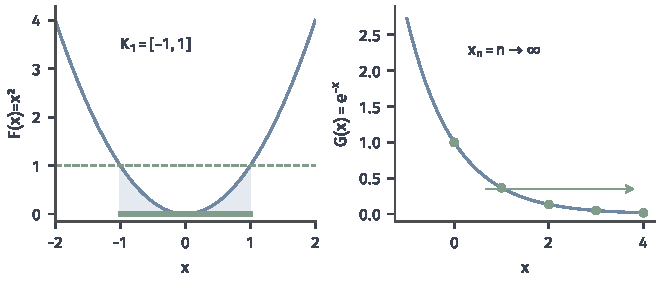
\includegraphics[width=112mm]{figures/00-shared/mathematical-preliminaries-upper/00-shared/matplotlib/mathematical-language-combinatorics-analysis-optimization-comprehension-additions/coercive-sublevels.pdf}
  \caption{全实线上的两个连续目标。左图$F(x)=x^2$的下水平集$K_1=\{x:F(x)\leq1\}=[-1,1]$有界；右图$G(x)=e^{-x}$沿$x_n=n$趋近下确界$0$，但没有最小点。左侧浅色仅标出下水平范围内的函数图下区域，绿线才表示参数集合$K_1$。这组例子说明存在性条件的职责，不声称强制性是任何最小点存在的必要条件。}
  \label{fig:vol1-add-coercive-sublevels}
\end{figure}

\noindent\begin{minipage}{\linewidth}
回到最小二乘：当$\lambda>0$时$F(\bm w)\geq\lambda\lVert\bm w\rVert_2^2/2$，在非空闭资源域上下水平集有界，故最小点存在。逐项回看各条件的职责：强制性留住有界性，闭域留住可行极限，下半连续把目标比较传到极限。它们都是充分条件；下一节增加的凸性仍须另行核验。

\section{凸性条件下的最优解性质}
\label{sec:opt-convexity}

存在性只回答“有没有”。本节依次加强三个条件：凸性把局部最优提升为全局最优，严格凸性排除多个最小点，强凸性再给出统一的曲率下界，把目标值差换算成参数距离。三者逐层增强，不能互相替代。

\subsection{凸性与全局最优}

\subsubsection{凸集、凸组合与凸函数}

\paragraph{远处更优点怎样影响局部比较}

局部最优只和附近候选比较。设想地形中有两个互相隔开的山谷：站在其中一个谷底向四周看，处处都更高，局部上已经最优，但另一个山谷可能更低，而局部信息里没有远处山谷的任何线索。如果任意两个可行点之间的线段都仍在可行域内，且沿这条线段的目标值不超过两端值的加权平均，那么远处一旦有更低的点，连向它的线段就会在当前点附近给出一个更低的点，“假谷底”随即被排除。这两项条件分别是集合与函数的凸性。
\end{minipage}\par
\begin{definition}[凸集与凸函数]
\label{def:opt-convex-set-function}
集合$C\subseteq\mathbb R^d$为\term{凸集}（convex set），是指对任意
$\bm{u},\bm{v}\in C$和$\theta\in[0,1]$，
$\theta\bm{u}+(1-\theta)\bm{v}\in C$。
定义在凸集$C$上的函数$f:C\to\mathbb R$若对任意$\bm u,\bm v\in C$和$\theta\in[0,1]$满足
\begin{equation}
  f(\theta\bm{u}+(1-\theta)\bm{v})
  \leq
  \theta f(\bm{u})+(1-\theta)f(\bm{v}),
  \label{eq:opt-convex-function}
\end{equation}
就称为\term{凸函数}（convex function）。若$-f$凸，则称$f$凹。
\end{definition}
线性等式、线性不等式和范数球的解集都是凸集，交集仍为凸集，所以式~\eqref{eq:opt-linear-resource-constraints}定义凸可行域。式~\eqref{eq:opt-convex-function}右侧是两个函数值的\term{加权平均}（weighted average）：两个系数非负且和为$1$，分别规定两端点值在平均中所占的份额。

\paragraph{有限凸组合、凸包与Jensen不等式}

二点线段可以反复使用。对非空集合$A\subseteq\mathbb R^d$中的有限个点$\bm a_1,\ldots,\bm a_m$，称
\[
  \sum_{i=1}^m\alpha_i\bm a_i,\qquad
  \alpha_i\geq0,\quad \sum_{i=1}^m\alpha_i=1
\]
为它们的凸组合；所有有限凸组合组成的集合记为$\operatorname{conv}(A)$。把“凸组合的凸组合”展开并合并权重，新权重仍非负且和为$1$，故$\operatorname{conv}(A)$凸；而任何包含$A$的凸集由二点组合归纳都包含全部有限凸组合，所以$\operatorname{conv}(A)$是包含$A$的最小凸集，即$A$的凸包。当$A$有限时，系数集合是闭有界的，线性加权映射连续，其像$\operatorname{conv}(A)$紧。凸包不默认闭：$A=(0,1)$的凸包仍是开区间$(0,1)$；若要把可逼近的极限也纳入，取闭凸包$\overline{\operatorname{conv}(A)}$，它是包含$A$的最小闭凸集。这两个对象将在松弛和梯度凸包投影中使用。

对凸域内的有限个点与凸函数，从二点凸性归纳得到\term{Jensen不等式}（Jensen's inequality）：
\begin{equation}
  f\left(\sum_{i=1}^m\alpha_i\bm{w}_i\right)
  \leq\sum_{i=1}^m\alpha_i f(\bm{w}_i).
  \label{eq:opt-jensen}
\end{equation}
归纳时先把前$m-1$个点的权重按$1-\alpha_m$归一化成一个加权平均，再与第$m$个点应用二点凸性；$\alpha_m=1$时直接是末点等式，避免除以零。非负与归一化不是装饰：允许负权重后组合点可能落到凸包之外，不等式不再有保证。

对扩展实值目标，式~\eqref{eq:opt-convex-function}只在有限取值的点上检验，并要求有效定义域凸，以免出现$0\cdot(+\infty)$的无意义运算。

\paragraph{扩展实值目标的凸性}

回到10.1节的统一形式：扩展实值凸函数的有效定义域必须凸，凸性不等式在两个端点都取有限值时检验，端点权重为零的情形按有效域约定处理。这里转换的只是函数的取值范围，有限凸组合的几何仍然是共同基础，不引入积分版Jensen。

\subsubsection{可微凸性的判据}

\paragraph{一阶支撑下界}

凸函数图像位于弦下方；可微时，它还位于每点切线的上方。

\begin{theorem}[凸函数的一阶与二阶判据]
\label{thm:opt-convexity-criteria}
设$C$为开凸集。可微函数$f:C\to\mathbb{R}$凸，当且仅当对任意
$\bm{u},\bm{v}\in C$，
\begin{equation}
  f(\bm{v})\geq f(\bm{u})
  +\langle\nabla f(\bm{u}),\bm{v}-\bm{u}\rangle.
  \label{eq:opt-first-order-convexity}
\end{equation}
若$f$二阶可微，则这又等价于
$\nabla^2f(\bm{w})\succeq\bm{0}$对所有$\bm{w}\in C$成立。
\end{theorem}

\begin{proof}
若$f$凸，沿线段令$\phi(t)=f(\bm{u}+t(\bm{v}-\bm{u}))$。由凸性，
$[\phi(t)-\phi(0)]/t\leq\phi(1)-\phi(0)$，令$t\downarrow0$便得
式~\eqref{eq:opt-first-order-convexity}。反过来，令
$\bm{z}=\theta\bm{u}+(1-\theta)\bm{v}$，分别把一阶不等式用于
$(\bm{z},\bm{u})$和$(\bm{z},\bm{v})$，乘以$\theta$与$1-\theta$后相加，
线性项抵消，恢复式~\eqref{eq:opt-convex-function}。

二阶情形：把一阶判据用于$\bm{w}$与$\bm{w}+t\bm{v}$，再对$t$取二阶局部极限，
得$\bm{v}^{\top}\nabla^2f(\bm{w})\bm{v}\geq0$。反之，沿任意线段定义
$\phi(t)$，则
$\phi''(t)=(\bm{v}-\bm{u})^{\top}\nabla^2f(\bm{u}+t(\bm{v}-\bm{u}))
(\bm{v}-\bm{u})\geq0$，一元函数$\phi$凸，故$f$凸。
\end{proof}

判据要求在整个开凸讨论域上成立：单个候选处Hessian半正定不能证明全域凸性，非开的约束域也不能不加说明地套用同样的导数陈述。图~\ref{fig:opt-convex-chord-tangent}把弦上界与切线下界画在一起，二者来自不同的比较对象，不能把某点的切线误当作连接两个函数值的弦\scite{math-boyd2004convex}。
\begin{figure}[htbp]
  \centering
  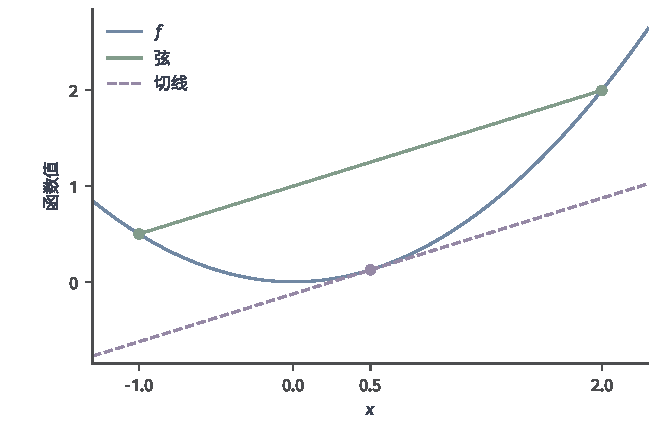
\includegraphics[width=112.0mm]{figures/00-shared/mathematical-preliminaries-upper/04-optimization/matplotlib/opt-convex-chord-tangent/figure.pdf}
  \caption{$f(x)=x^2/2$的弦与切线。蓝线为函数，绿线连接$u=-1$与$v=2$的函数值，
 在这两个输入之间给出弦上界；紫虚线是在$x_0=1/2$处的一阶仿射下界，适用于整个实线。
 绿线的上界只在其端点之间使用，切线下界来自凸性。图为解析教学示例。}
 \label{fig:opt-convex-chord-tangent}
\end{figure}

\subsubsection{局部最优与驻点的全局意义}

凸性把局部比较提升为全局比较。设凸域中局部最小点$\bm u$不是全局最小点，取$\bm v\in C$使$f(\bm v)<f(\bm u)$，则对任意$t\in(0,1)$，
\[
  f(\bm u+t(\bm v-\bm u))
  \leq(1-t)f(\bm u)+tf(\bm v)<f(\bm u),
\]
取足够小的$t$，新点仍在局部比较邻域内，与局部最优矛盾。这个证明不要求可微，所以对凸的非光滑目标也成立。对无约束可微凸目标，把$\nabla f(\bm w^\star)=\bm0$代入式~\eqref{eq:opt-first-order-convexity}便得$f(\bm v)\geq f(\bm w^\star)$，因此凸问题的驻点就是全局最小点；反过来，非凸问题找到驻点只能说明附近没有一阶下降方向。边界上的约束最优点并不要求普通梯度为零。

\subsection{严格凸性与解的唯一性}

凸函数可以沿某个方向保持不变，所以“局部即全局”并没有排除多个最小点。最小点不唯一时，返回哪个解取决于算法路径，与最小点距离有关的误差界也无从定义。

\begin{definition}[严格凸函数]
\label{def:opt-strict-convexity}
设$C$凸，$f:C\to\mathbb R$。若式~\eqref{eq:opt-convex-function}对所有
$\bm u\neq\bm v$及$0<\theta<1$严格成立，则称$f$严格凸。
\end{definition}

若两个不同点$\bm u,\bm v$都达到最小值$m$，严格凸性使其中点的函数值严格小于$(m+m)/2=m$，矛盾。因此严格凸只保证最小点至多一个：严格凸函数$e^x$在实线上就没有最小点，存在性仍须交给10.2节合用。反方向也不成立：$|x|$有唯一最小点，但在同号线段上是仿射、并不严格凸，所以不能由解唯一反推严格凸。

回到式~\eqref{eq:opt-regularized-least-squares}：$\lambda=0$且$\bm X$不满列秩时，沿零空间方向目标不变，存在一整条最优线段；$\bm X$满列秩或$\lambda>0$时，任意非零方向$\bm d$都有$\|\bm X\bm d\|_2^2/n+\lambda\|\bm d\|_2^2>0$，目标严格凸。再与闭可行域上的存在性合用，才能断言解唯一。

\subsection{强凸性与误差几何}
\label{sec:opt-strong-convex}

严格凸只要求“中点严格更低”，没有规定低多少：两个严格凸函数可以一个像浅口碗、一个像深漏斗。这个“低多少”决定目标误差能换回多小的参数误差，也决定后面梯度类算法收敛得多快。强凸性要求弦段与函数之间至少留出一个与距离平方成比例的间隔。它是目标自身的误差几何，尚不涉及算法的迭代速度。

\subsubsection{相对于范数的统一曲率下界}

\begin{definition}[相对于范数的强凸性]
\label{def:opt-strong-convexity}
设$C$是实赋范空间中的凸集，$f:C\to\mathbb{R}$，$\mu>0$。若对任意
$\bm{u},\bm{v}\in C$和$\theta\in[0,1]$都有
\begin{equation}
 f(\theta\bm{u}+(1-\theta)\bm{v})
 \leq\theta f(\bm{u})+(1-\theta)f(\bm{v})
 -\frac{\mu}{2}\theta(1-\theta)\lVert\bm{u}-\bm{v}\rVert^2,
 \label{eq:opt-norm-strong-convexity}
\end{equation}
则称$f$相对于$\lVert\cdot\rVert$是\term{$\mu$强凸}（$\mu$-strongly convex）的。
\end{definition}

这个定义可以容纳非光滑正则项和欧氏范数以外的范数：$|x|+\mu x^2/2$虽在$0$处不可微，仍相对于绝对值范数$\mu$强凸——绝对值部分提供凸性，二次部分恰好补上式~\eqref{eq:opt-norm-strong-convexity}中的距离平方间隔。而$x^4$严格凸，却在原点曲率为零、给不出全域统一的二次下界，说明强凸增加的是定量条件。

在欧氏空间的开凸集上，若$f$可微，对$f-\mu\|\cdot\|_2^2/2$应用凸性判据，强凸性等价于
\begin{equation}
  f(\bm{v})\geq f(\bm{u})+
  \langle\nabla f(\bm{u}),\bm{v}-\bm{u}\rangle
  +\frac{\mu}{2}\lVert\bm{v}-\bm{u}\rVert_2^2;
  \label{eq:opt-first-order-strong-convexity}
\end{equation}
二阶可微时又等价于$\nabla^2f(\bm w)\succeq\mu\bm I$。一般范数的平方未必是欧氏二次型，所以不能把Hessian写法当作所有范数下的通用定义。对最小二乘可直接读出Hessian为$\bm X^\top\bm X/n+\lambda\bm I$：$\lambda>0$时目标至少$\lambda$强凸；秩亏且无正则时仍凸，却取不到正的强凸常数。

\subsubsection{目标差控制到最小点的距离}

设凸域中最小点$\bm w^\star$已存在。把强凸定义用于$\bm w^\star$与任意可行$\bm w$，并用最优性给线段上的函数值加下界：对任意$t\in(0,1)$，
\[
 f(\bm w^\star)\leq(1-t)f(\bm w^\star)+tf(\bm w)
 -\frac{\mu}{2}t(1-t)\|\bm w-\bm w^\star\|^2.
\]
除以$t>0$再令$t\downarrow0$，得到
\begin{equation}
 f(\bm w)-f(\bm w^\star)\geq\frac{\mu}{2}\|\bm w-\bm w^\star\|^2,
 \qquad
 \|\bm w-\bm w^\star\|\leq\sqrt{\frac{2(f(\bm w)-f^\star)}{\mu}}.
 \label{eq:opt-strong-convex-distance}
\end{equation}
这同时排除了不同的最小点，并把目标精度换算成参数精度。证明没有假设最优点在内部或目标可微，因此对固定凸域边界上的非光滑强凸目标同样成立；它仍未回答算法取得该目标精度需要多少轮——那是第11章的问题。最优解对问题扰动（线性项变化、约束参数变化）的响应将分别在11.5和13.8讨论。

\section{本章小结}

本章围绕同一个候选区分了五件事：可行性、达到性、全局或局部最优、驻点残差，以及目标差、参数距离、预测差三种误差。存在、唯一和误差大小分别回答不同问题：紧域上连续目标达到最小值，闭域上适当、下半连续且强制的目标通过紧下水平集达到最小值；凸性把局部最优提升为全局最优，严格凸把最小点限制为至多一个，强凸再用统一常数把目标差换算成参数距离。唯一性既不保证数值稳定，也不决定算法速度，指定尺度下的扰动分析要到11.5节。

本章始终没有生成任何迭代序列。下一章起，我们才把局部导数、曲率常数和这里的误差关系放进更新过程：方法说明当前困难、改变的机制和执行步骤，再检验每一步与有限预算下的保证；不能由本章的问题性质直接推断任意算法都能取得相同结果。

\chapter{无约束光滑目标的求解}
\label{chap:smooth-optimization}

本章只考虑无约束、目标可微的优化问题。有了第10章可判定的最优性条件，还需构造能逐步接近它的参数序列。为了把不同方法放在同一把尺子下比较，本章反复使用
\begin{equation}
 f(\bm w)=\frac12(w_1^2+16w_2^2),\qquad
 \bm H=\operatorname{diag}(1,16),\qquad
 \bm w^{(0)}=(2,2)^\top.
 \label{eq:opt-common-quadratic}
\end{equation}
它的最小点为零，初始目标值为$34$，两个坐标方向的曲率相差$16$倍，使每种方法的方向、步长和每步成本都能直接核算。

本章的前半介绍方法，后半回答四个共同问题。11.1节从梯度及历史形成方向：普通梯度下降、固定预条件、动量与符号方向、逐坐标历史缩放，以及矩阵方向变换；11.2节用局部模型给出候选步：牛顿族、Gauss--Newton族、拟牛顿，以及按模型输出变化度量位移的自然梯度；11.3节处理学习率、参数衰减和执行次序。方向构造、模型求解与更新控制是三种可组合的职责，而不是互斥的算法类别。11.4节比较收敛速度与计算成本，11.5节分析数值误差传播和最优解对扰动的敏感性，11.6节讨论非最小驻点与逃离鞍点，11.7节解释优化路径在多解问题中的隐式偏置。

阅读方法部分时应能据输入写出一轮更新并说出返回什么；性质部分再判断下降、收敛速度、计算量与解的选择。平方梯度的非中心二阶矩不是目标Hessian，矩阵乘法也不自动意味着使用了二阶信息。抽样与小批量在第14章讨论；本章的梯度都是同一明确目标的真实梯度。

\section{基于梯度的方向构造}
\label{sec:opt-first-order-methods}

本节回答“怎样把当前及历史梯度变成一个可执行方向”。统一记第$t$轮参数为$\bm w^{(t)}$、$\bm g^{(t)}=\nabla f(\bm w^{(t)})$，逐坐标向量运算以$\odot$表示逐元素乘法。给定预算和精度标准后，方法返回实际参数点及所需历史状态；停止时核验原目标或真实梯度，不能把平滑后方向小、步长缩小或参数位移小当作证书。

\subsection{梯度下降与回溯步长}
\label{sec:opt-gradient-descent}

对可求梯度的有限维实值目标$f:\mathbb R^d\to\mathbb R$，梯度给出当前点最陡的上升方向，梯度下降取其反向：
\begin{equation}
  \bm{w}^{(t+1)}=\bm{w}^{(t)}-\eta^{(t)}\nabla f(\bm{w}^{(t)}).
  \label{eq:opt-gradient-descent}
\end{equation}
沿负梯度走“足够小”的一步一定下降：函数值变化的一阶近似为$-\eta\|\nabla f\|_2^2<0$。问题在于“足够小”没有可事先使用的尺度；位移越大，被舍弃的高阶项影响越大。要把它换成可计算的步长范围，需要控制移动后梯度改变多少。

\begin{definition}[欧氏梯度光滑性]
\label{def:opt-smoothness}
设$f:\mathbb R^d\to\mathbb R$可微，$L\geq0$有限。若对任意$\bm u,\bm v$都有
$\lVert\nabla f(\bm{u})-\nabla f(\bm{v})\rVert_2
\leq L\lVert\bm{u}-\bm{v}\rVert_2$，
则称$f$为\term{$L$光滑}（$L$-smooth）。
\end{definition}

常数$L$给“每移动单位距离，梯度最多改变多少”定了上限。沿线段积分即可得到控制一阶模型余项的下降引理。

\begin{lemma}[下降引理]
\label{lem:opt-descent}
若$f$可微且梯度是$L$-Lipschitz连续的，$L>0$，则对任意$\bm u,\bm v$，
\begin{equation}
  f(\bm{v})\leq f(\bm{u})
  +\langle\nabla f(\bm{u}),\bm{v}-\bm{u}\rangle
  +\frac{L}{2}\lVert\bm{v}-\bm{u}\rVert_2^2.
  \label{eq:opt-descent-lemma}
\end{equation}
\end{lemma}

\begin{proof}
令$\bm d=\bm v-\bm u$。沿线段积分并减去一阶项：
\[
  f(\bm v)-f(\bm u)-\langle\nabla f(\bm u),\bm d\rangle
  =\int_0^1\langle\nabla f(\bm u+t\bm d)-\nabla f(\bm u),\bm d\rangle\,\mathrm dt.
\]
由Cauchy--Schwarz不等式与梯度Lipschitz条件，被积函数至多为$Lt\|\bm d\|_2^2$，积分即得结论。
\end{proof}

把更新式代入下降引理，得到单步下降
\begin{equation}
  f(\bm{w}^{(t+1)})
  \leq f(\bm{w}^{(t)})
  -\eta^{(t)}\left(1-\frac{L\eta^{(t)}}2\right)
  \lVert\nabla f(\bm{w}^{(t)})\rVert_2^2.
  \label{eq:opt-gradient-single-step}
\end{equation}
所以$0<\eta<2/L$保证每个非驻点处严格下降；取典型值$\eta=1/L$。若$f$下有界，记$f_{\inf}=\inf f>-\infty$，对$t=0,\ldots,T-1$求和，得到非凸光滑情形的有限预算保证
\begin{equation}
  \min_{0\leq t<T}\lVert\nabla f(\bm{w}^{(t)})\rVert_2^2
  \leq
  \frac{2L(f(\bm{w}^{(0)})-f_{\inf})}{T}.
  \label{eq:opt-nonconvex-gradient-rate}
\end{equation}
它只说明某次迭代接近驻点，没有声称驻点是全局最优点；对应梯度范数容差$\varepsilon$的评价次数为$O(\varepsilon^{-2})$。

步长边界在一维二次函数上就能看到。对$f(w)=Lw^2/2$，迭代为$w^{(t+1)}=(1-\eta L)w^{(t)}$：$\eta=2/L$时在正负之间等幅振荡，$\eta>2/L$时幅度按$|1-\eta L|>1$增长。负梯度方向本身没错，失败来自步长跨过了曲率允许的稳定范围。

图~\ref{fig:vol1-add-gradient-step-stability}用同一初值比较四个步长。
\begin{figure}[!htb]
  \centering
  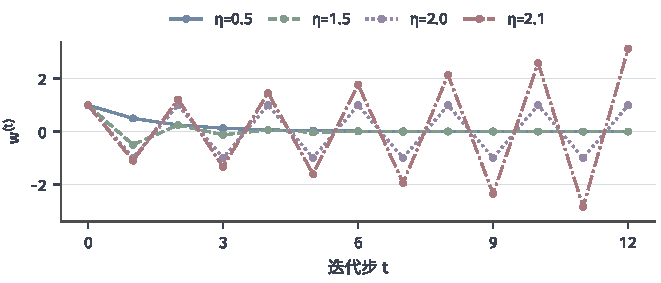
\includegraphics[width=112mm]{figures/00-shared/mathematical-preliminaries-upper/00-shared/matplotlib/mathematical-language-combinatorics-analysis-optimization-comprehension-additions/gradient-step-stability.pdf}
  \caption{对$f(w)=w^2/2$取$w^{(0)}=1$，画精确迭代$w^{(t)}=(1-\eta)^t$。$\eta=0.5$同侧收缩，$\eta=1.5$换侧收缩，$\eta=2$等幅振荡，$\eta=2.1$幅度增长。各点仅对应整数步，连线帮助追踪次序。这里$L=1$，稳定边界正是$2/L$。}
  \label{fig:vol1-add-gradient-step-stability}
\end{figure}

\paragraph{回溯线搜索。}
固定步长需要已知或估计$L$：估计偏大则步长过小、收敛变慢，估计偏小则下降保证失效。不依赖$L$具体数值的做法是用实际函数值检验这一步是否真的下降。给定初始试探步长$\bar\eta>0$、缩减比例$\gamma\in(0,1)$与$c\in(0,1)$，回溯线搜索从$\eta=\bar\eta$开始缩小，直到
\[
  f(\bm w-\eta\nabla f(\bm w))
  \leq f(\bm w)-c\eta\|\nabla f(\bm w)\|_2^2
\]
成立。下降引理保证$\eta\leq2(1-c)/L$时一定通过，所以全局$L$光滑时每轮有限次结束，接受步长至少为$\min\{\bar\eta,2\gamma(1-c)/L\}$。增加的成本主要是试探点函数求值。学习率调度则预先或按读数改变$\eta^{(t)}$，集中放在11.3节；两者都不能弥补错误梯度或无下界目标。

\paragraph{凸目标上的目标差。}
若$f$还凸、最小点$\bm w^\star$存在，继续取$\eta=1/L$。由凸性$f(\bm w^{(t)})-f^\star\leq\langle\nabla f(\bm w^{(t)}),\bm w^{(t)}-\bm w^\star\rangle$，结合距离平方递推和式~\eqref{eq:opt-gradient-single-step}消去梯度平方项，望远镜求和可得
\begin{equation}
  f(\bm{w}^{(T)})-f^\star
  \leq\frac{L\lVert\bm{w}^{(0)}-\bm{w}^{\star}\rVert_2^2}{2T}.
  \label{eq:opt-convex-gradient-rate}
\end{equation}

\paragraph{PL条件下的几何速度。}
\term{Polyak--Łojasiewicz条件}（PL condition）不要求函数凸，而用梯度大小控制目标差。

\begin{definition}[Polyak--Łojasiewicz条件]
\label{def:opt-pl-condition}
设$f$可微，$f^\star=\inf f>-\infty$。若存在$\mu>0$，使任意$\bm w$满足
\begin{equation}
  \frac{1}{2}\lVert\nabla f(\bm{w})\rVert_2^2
  \geq \mu\bigl(f(\bm{w})-f^{\star}\bigr),
  \label{eq:opt-pl-condition}
\end{equation}
则称$f$满足常数为$\mu$的PL条件。
\end{definition}

$\mu$强凸可微函数把式~\eqref{eq:opt-first-order-strong-convexity}右侧关于$\bm v$最小化即推出PL条件；反过来PL函数可以有多个最小点，也可以不凸。例如$f(x,y)=x^2+2\sin^2x$与$y$无关、最小点不唯一，$\partial^2 f/\partial x^2=2+4\cos2x$在某些点为负，却可验证存在$\mu>0$满足式~\eqref{eq:opt-pl-condition}。取$\eta=1/L$（必要时把常数减小到$\mu\leq L$），单步下降与PL条件给出几何收缩
\begin{equation}
  f(\bm{w}^{(t)})-f^\star
  \leq\left(1-\frac{\mu}{L}\right)^t
  \bigl(f(\bm{w}^{(0)})-f^\star\bigr).
  \label{eq:opt-pl-linear-rate}
\end{equation}
没有强凸时，这条界不保证迭代趋向某个唯一参数；已知PL常数时，$\|\nabla f\|_2\leq\sqrt{2\mu\varepsilon}$足以保证目标差不超过$\varepsilon$，但这条停止规则不能无条件用于所有光滑目标。

\paragraph{共同二次例上的逐方向核对。}
在式~\eqref{eq:opt-common-quadratic}中取$\eta=1/16$，$t\geq1$时$\bm w^{(t)}=(2(15/16)^t,0)^\top$，第二坐标一步消去，第一坐标却受较大曲率限制而缓慢缩小；$\eta=0.1$使两坐标分别乘$0.9$与$-0.6$，目标仍下降但路径振荡；$\eta=1/8$使第二坐标等幅振荡，更大则发散。一般非凸问题返回梯度范数最小的已访问点，凸问题可返回最后一点。

\subsection{固定预条件与坐标变换}

普通梯度下降用同一个标量步长，同时受陡方向的稳定限制和平坦方向的缓慢推进牵制。对固定正定矩阵$\bm P$，可以按
\begin{equation}
  \bm{w}^{(t+1)}=\bm{w}^{(t)}-\eta\bm P\nabla f(\bm{w}^{(t)})
  \label{eq:opt-fixed-precondition}
\end{equation}
重新缩放方向，这称为\term{预条件}（preconditioning）。令$\bm w=\bm P^{1/2}\bm z$，它就是新坐标下的普通梯度下降；$\bm P$不改变原目标数值，步长与停止仍按原目标选择。

对正定二次目标，变换后的曲率为$\widetilde{\bm H}=\bm P^{1/2}\bm H\bm P^{1/2}$。原坐标误差递推$(\bm I-\eta\bm P\bm H)$与新坐标递推$(\bm I-\eta\widetilde{\bm H})$相似，故特征值相同；迭代收敛当且仅当$0<\eta<2/\lambda_{\max}(\widetilde{\bm H})$，取$\eta=2/(\widetilde L+\widetilde\mu)$时每步最坏收缩因子为$(\widetilde\kappa-1)/(\widetilde\kappa+1)$，其中$\widetilde\kappa=\widetilde L/\widetilde\mu$。因此预条件的目标不是让$\bm P$自身条件数小，而是让变换后曲率$\widetilde{\bm H}$的条件数接近$1$；$\bm P$与$\bm H$不匹配时条件数反而可能增大。这一分析只针对固定$\bm P$，随历史变化的缩放矩阵必须另行说明构造与正定性。

\begin{example}[两个曲率方向上的预条件]
\label{ex:opt-anisotropic-preconditioning}
取共同二次目标、初值$(2,2)^\top$。普通梯度下降取$\eta=0.1$时两坐标分别乘以$0.9$与$-0.6$，第二坐标来回越过谷底。取$\bm P=\operatorname{diag}(1,1/16)$及$\eta=1/2$后，$\bm P\nabla f(\bm w)=\bm w$，两坐标每步都减半。
\end{example}

\begin{figure*}[htbp]
  \centering
  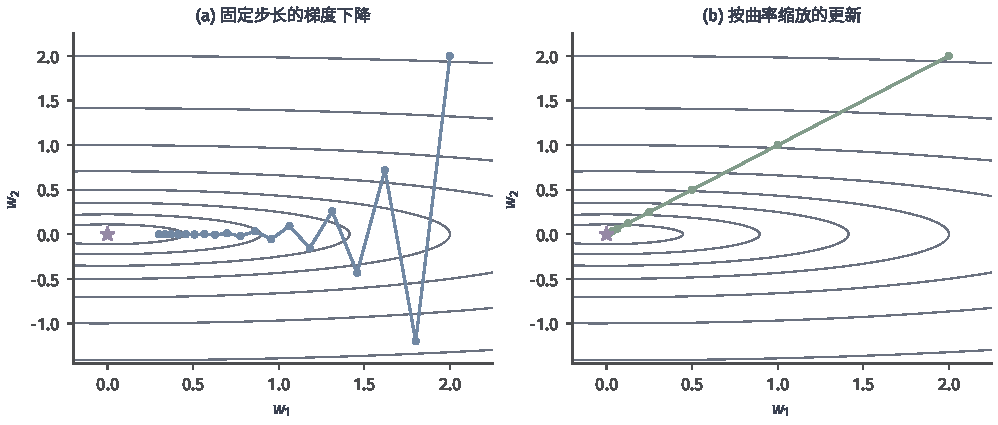
\includegraphics[width=169.0mm]{figures/00-shared/mathematical-preliminaries-upper/04-optimization/matplotlib/opt-preconditioned-paths/figure.pdf}
  \caption{例~\ref{ex:opt-anisotropic-preconditioning}中的精确更新路径。灰线是同一二次目标的等值线，蓝、绿圆点分别表示普通更新与预条件更新，星号是最小点。预条件使用了已知曲率，获得和应用这一矩阵的成本仍属于算法代价。}
 \label{fig:opt-preconditioned-paths}
\end{figure*}

\subsection{动量与符号方向}

这一组方法保留梯度方向或参数位移的历史。先看重球与Nesterov如何混合旧方向、在哪个点求新梯度，再看只保留符号的Lion。

\subsubsection{重球动量法}

在狭长谷底上，梯度方向在两侧之间来回摆动，真正指向谷底的分量每步却很小；想象小球在又陡又窄的滑槽里下滑，大部分动能用于撞击两壁。对连续几步指向同一侧的梯度取平均，摆动分量相消，这就是动量的作用。\term{动量法}（momentum method）的重球（heavy-ball）形式为
\[
  \bm v^{(t+1)}=\beta\bm v^{(t)}+\nabla f(\bm w^{(t)}),
  \qquad
  \bm w^{(t+1)}=\bm w^{(t)}-\eta\bm v^{(t+1)},
\]
取$\bm v^{(0)}=\bm0$启动，每轮只增加一次向量加法，不增加梯度求值。

对正定二次目标$f=\frac12\bm w^\top\bm H\bm w-\bm c^\top\bm w$，消去$\bm v$后，曲率为$\lambda_i$的特征方向上误差满足二阶递推
\[
  e_i^{(t+1)}=(1+\beta-\eta\lambda_i)e_i^{(t)}-\beta e_i^{(t-1)}.
\]
由特征多项式的Jury判据，$0\leq\beta<1$时两根都在单位圆内当且仅当$0<\eta\lambda_i<2(1+\beta)$，故所有方向稳定要求$0<\eta<2(1+\beta)/L$。已知谱界$[\mu,L]$时的经典参数为
\[
  \eta=\frac{4}{(\sqrt L+\sqrt\mu)^2},\qquad
  \beta=\left(\frac{\sqrt L-\sqrt\mu}{\sqrt L+\sqrt\mu}\right)^2,
\]
最坏方向根模至多$q=(\sqrt L-\sqrt\mu)/(\sqrt L+\sqrt\mu)$，端点重根还带来$tq^t$因子。它们是二次模型上的参数，不是一般非凸或含噪梯度下的无条件调参规则；启动阶段目标甚至可能上升——在共同二次例上取$\eta=4/25$、$\beta=9/25$，第一步目标便从$34$升至$79.2864$，之后才趋于零。

\subsubsection{Nesterov加速梯度法}

重球在当前点求梯度，其二阶递推不能直接给出一般凸目标的加速证明。\term{Nesterov加速梯度}（Nesterov accelerated gradient）改变求导位置：先外推，再在前瞻点求梯度。对凸、$L$光滑、最小点存在的目标，初始化$\bm z^{(0)}=\bm w^{(0)}$、$q^{(0)}=1$，依次计算
\begin{align*}
 \bm w^{(t+1)}&=\bm z^{(t)}-\frac1L\nabla f(\bm z^{(t)}),&
 q^{(t+1)}&=\frac{1+\sqrt{1+4(q^{(t)})^2}}2,\\
 \bm z^{(t+1)}&=\bm w^{(t+1)}
 +\frac{q^{(t)}-1}{q^{(t+1)}}(\bm w^{(t+1)}-\bm w^{(t)}).
\end{align*}
必须先得到新点，再形成下一轮前瞻点。在精确梯度与步长$1/L$下，
\begin{equation}
 f(\bm w^{(T)})-f^\star
 \leq\frac{2L\|\bm w^{(0)}-\bm w^\star\|_2^2}{(T+1)^2},
 \label{eq:opt-accelerated-finite-rate}
\end{equation}
而普通梯度下降的一般保证是$O(1/T)$。

证明用势函数把目标差与到最小点的距离合在一起。下降引理与凸性给出对任意$\bm v$成立的三点不等式
\[
 f(\bm x^+)-f(\bm v)
 \leq\frac L2\bigl(\|\bm v-\bm z\|_2^2-\|\bm v-\bm x^+\|_2^2\bigr),
 \qquad \bm x^+=\bm z-\frac1L\nabla f(\bm z).
\]
选比较点$\bm v=(1-1/q^{(t)})\bm w^{(t)}+\bm w^\star/q^{(t)}$，再用辅助点$\bm u^{(t)}$把外推位移并入同一向量，可使加权目标差与距离平方组成的量
\[
 E^{(t)}=(q^{(t-1)})^2\Delta^{(t)}
 +\frac L2\|\bm u^{(t)}-\bm w^\star\|_2^2
\]
逐步不增；启动的两次比较$E^{(1)}\leq E^{(0)}$、$E^{(2)}\leq E^{(1)}$可直接核验，一般步的衔接依赖恒等式$q^{(t)}(q^{(t)}-1)=(q^{(t-1)})^2$。由$q^{(T-1)}\geq(T+1)/2$即得式~\eqref{eq:opt-accelerated-finite-rate}。目标未必逐轮单调，一般凸情形也没有规定唯一参数；未知$L$时须配合与加速方案一致的回溯。神经网络实现中另常用固定$\beta$的前瞻变体（先令$\bar{\bm w}^{(t)}=\bm w^{(t)}-\eta_t\beta\bm m^{(t)}$，再在$\bar{\bm w}^{(t)}$求梯度更新缓冲），它与上述$q^{(t)}$方案不是同一算法，不自动继承$O(1/T^2)$界。

\subsubsection{Lion符号动量法}

若希望用历史向量形成方向、又不保留逐坐标平方统计，可以在混合梯度后只取符号。\term{Lion}取$\bm m^{(0)}=\bm0$、$\beta_1,\beta_2\in[0,1)$、$\eta_t>0$、$\lambda\geq0$，每轮先算方向$\bm z^{(t)}=\beta_1\bm m^{(t)}+(1-\beta_1)\bm g^{(t)}$，再更新并保存
\[
 \bm w^{(t+1)}=(1-\eta_t\lambda)\bm w^{(t)}
 -\eta_t\operatorname{sign}(\bm z^{(t)}),\qquad
 \bm m^{(t+1)}=\beta_2\bm m^{(t)}+(1-\beta_2)\bm g^{(t)},
\]
约定$\operatorname{sign}(\bm0)=\bm0$。方向使用旧缓冲，不能先用$\beta_2$覆盖状态。符号丢弃混合梯度的幅度：不计衰减时，若本轮有$q$个非零符号，位移范数恰为$\eta_t\sqrt q$，所以相同步长数值不代表与梯度下降或Adam相同的总位移。独立衰减项的目标解释与AdamW一样需要另行核对。

\subsection{逐坐标历史缩放}
\label{sec:opt-per-coordinate-scaling}

这一组方法按坐标记录梯度幅度，再以这些记录决定各坐标的缩放。AdaGrad累计全部历史，RMSProp改用衰减平均，AdaDelta再记录更新幅度，Adam加入方向平均，AMSGrad约束分母只增不减，AdamW把参数衰减移出统计，Adafactor压缩矩阵参数的平方表。

\subsubsection{AdaGrad}

对梯度幅度在坐标间差异明显的问题，AdaGrad累计平方梯度并按累计尺度缩放。取$\bm v^{(0)}=\bm0$、$\eta>0$、$\epsilon>0$：
\[
 \bm v^{(t+1)}=\bm v^{(t)}+\bm g^{(t)}\odot\bm g^{(t)},\qquad
 \bm w^{(t+1)}=\bm w^{(t)}
 -\frac{\eta\bm g^{(t)}}{\sqrt{\bm v^{(t+1)}}+\epsilon}.
\]
若某坐标每轮梯度同为非零$g$，忽略稳定项时第$t+1$次位移幅度约为$\eta/\sqrt{t+1}$；稀疏坐标只在实际非零时增加累计量。累计量不减，不能主动忘记早期大梯度；这里采用根号外加稳定项的版本，不与根号内加常数的实现混用。

\subsubsection{RMSProp}

为让近期梯度替换不可遗忘的累计历史，RMSProp取衰减平均：
\[
 \bm v^{(t+1)}=\rho\bm v^{(t)}+(1-\rho)\bm g^{(t)}\odot\bm g^{(t)},\qquad
 \bm w^{(t+1)}=\bm w^{(t)}
 -\eta_t\frac{\bm g^{(t)}}{\sqrt{\bm v^{(t+1)}}+\epsilon},
\]
其中$\rho\in[0,1)$。恒定坐标梯度给$\bm v^{(t+1)}=(1-\rho^{t+1})g^2$，零初始化使早期分母小于稳态；较大的$\rho$保留历史更久，也延缓响应。它只记录当前坐标系中的逐坐标幅度，不描述坐标间的耦合曲率。

\subsubsection{AdaDelta}

AdaDelta同时保存平方梯度平均$\bm v$和平方更新平均$\bm r$，取$\bm v^{(0)}=\bm r^{(0)}=\bm0$：
\[
 \bm v^{(t+1)}=\rho\bm v^{(t)}+(1-\rho)\bm g^{(t)}\odot\bm g^{(t)},
\]
\[
 \bm\Delta^{(t)}
 =-\frac{\sqrt{\bm r^{(t)}+\epsilon}}{\sqrt{\bm v^{(t+1)}+\epsilon}}
 \odot\bm g^{(t)},
\]
\[
 \bm r^{(t+1)}=\rho\bm r^{(t)}+(1-\rho)\bm\Delta^{(t)}\odot\bm\Delta^{(t)},
\]
\[
 \bm w^{(t+1)}=\bm w^{(t)}+\bm\Delta^{(t)}.
\]
分子必须用旧的$\bm r^{(t)}$，否则本步增量被循环定义；两个稳定项都在根号内，$\epsilon$还承担零状态启动作用。这里选原论文不另乘全局学习率的版本；省去独立学习率不等于省去$\rho$、$\epsilon$和初值选择。

\subsubsection{Adam}

Adam把方向平均与逐坐标幅度调整组合。取$\bm m^{(0)}=\bm v^{(0)}=\bm0$、$\beta_1,\beta_2\in[0,1)$：
\begin{align*}
 \bm m^{(t+1)}&=\beta_1\bm m^{(t)}+(1-\beta_1)\bm g^{(t)},&
 \bm v^{(t+1)}&=\beta_2\bm v^{(t)}+(1-\beta_2)\bm g^{(t)}\odot\bm g^{(t)},\\
 \widehat{\bm m}^{(t+1)}&=\frac{\bm m^{(t+1)}}{1-\beta_1^{t+1}},&
 \widehat{\bm v}^{(t+1)}&=\frac{\bm v^{(t+1)}}{1-\beta_2^{t+1}},
\end{align*}
\[
 \bm w^{(t+1)}=\bm w^{(t)}
 -\eta_t\frac{\widehat{\bm m}^{(t+1)}}{\sqrt{\widehat{\bm v}^{(t+1)}}+\epsilon}.
\]
把一阶递推展开为权重和为$1-\beta_1^{t+1}$的有限几何和，就看出偏差修正的作用：恒定梯度序列恰好恢复该梯度；这不需要概率前置，也不表示非平稳历史等于当前梯度。首步修正后非零坐标在忽略稳定项时呈符号步。历史为两组$d$维向量和步数，恢复训练须一并恢复这些状态；稳定项排除零分母，却不使方向映射自动具有统一Lipschitz常数。

正分母的连续性需要单独核验。以一个坐标的$m/(\sqrt v+\varepsilon)$为例，通分后用$|\sqrt v-\sqrt{\widetilde v}|\leq\sqrt{|v-\widetilde v|}$，方向差可由$|m-\widetilde m|/\varepsilon$与$\sqrt{|v-\widetilde v|}$的项控制；只有另有$v,\widetilde v\geq v_{\min}>0$时，才得到对$v$差的线性界。分母可算、扰动连续、统一Lipschitz是三个不同条件，不能以稳定项代替敏感度分析。

\subsubsection{AMSGrad}

Adam的平方平均会遗忘历史，分母可能回落。AMSGrad增加逐坐标历史最大值，采用不做零初始化修正的基本版本，在$\bm m,\bm v$的Adam递推之外取
\[
 \bar{\bm v}^{(t+1)}=\max(\bar{\bm v}^{(t)},\bm v^{(t+1)}),\qquad
 \bm w^{(t+1)}=\bm w^{(t)}
 -\eta_t\frac{\bm m^{(t+1)}}{\sqrt{\bar{\bm v}^{(t+1)}}+\epsilon}.
\]
逐坐标$\bar{\bm v}$不减，若$\eta_t$也不增，分母尺度对应的有效系数不增；这是代数性质，既不是目标值单调，也不是无条件的非凸收敛证明——原论文的在线凸分析另有有界域、梯度界和步长日程要求。带偏差修正的库版本须说明最大值作用在修正前还是修正后。

\subsubsection{AdamW与独立参数衰减}

若希望独立控制参数收缩、又不让衰减进入Adam的历史统计，给定数据目标$f$，仍以$\bm g^{(t)}=\nabla f(\bm w^{(t)})$执行$\bm m,\bm v$及修正，再令
\[
 \bm w^{(t+1)}=(1-\eta_t\lambda)\bm w^{(t)}
 -\eta_t\frac{\widehat{\bm m}^{(t+1)}}{\sqrt{\widehat{\bm v}^{(t+1)}}+\epsilon},
 \qquad 0\leq\eta_t\lambda<1.
\]
衰减不进入$\bm m,\bm v$，与把$\lambda\|\bm w\|_2^2/2$加到目标再运行Adam不同：后者把$\bm g+\lambda\bm w$同时送进方向与平方统计。一维首步即可复算差异：$w^0=1$、数据梯度为零、$\eta_0=0.1$、$\lambda=2$、$\epsilon=1$时，AdamW得$w^1=0.8$，对加L2目标的Adam得$14/15$。独立衰减不是固定欧氏L2目标的精确求解器；只对部分参数衰减时，所选坐标与系数必须作为算法输入给出。

\subsubsection{Adafactor}

矩阵参数的完整平方梯度表占用$O(md)$存储。Adafactor只维护行、列边际来近似它。固定参数块$\bm W^{(t)}\in\mathbb R^{m\times d}$与同点梯度$\bm D^{(t)}$，行、列状态初始为零，令$A_{ij}=(D_{ij})^2+\epsilon_1$，按
\[
 r_i^{t+1}=b_t r_i^t+(1-b_t)\frac1d\sum_jA_{ij}^t,\qquad
 c_j^{t+1}=b_t c_j^t+(1-b_t)\frac1m\sum_iA_{ij}^t
\]
更新，再重构
\[
 \widehat V_{ij}^{t+1}
 =\frac{r_i^{t+1}c_j^{t+1}}{m^{-1}\sum_k r_k^{t+1}}.
\]
同一衰减保持行列总均值一致，$\epsilon_1>0$与$b_t<1$保证重构分母为正。得到$\bm U^t=\bm D^t/\sqrt{\widehat V^{t+1}}$后，按$\operatorname{RMS}(\bm B)=\sqrt{(md)^{-1}\sum_{ij}B_{ij}^2}$把更新裁剪为$\widetilde{\bm U}^t=\bm U^t/\max\{1,\operatorname{RMS}(\bm U^t)/c_{\rm clip}\}$，取相对步长$\alpha_t=\rho_t\max\{\epsilon_2,\operatorname{RMS}(\bm W^t)\}$，令$\bm W^{t+1}=\bm W^t-\alpha_t\widetilde{\bm U}^t$。裁剪的是预条件后的更新；参数近零时$\epsilon_2$给出非零尺度。一个可执行的日程例为$b_t=1-(t+1)^{-0.8}$、$\rho_t=\min\{10^{-2},(t+1)^{-1/2}\}$。无完整动量时历史存储为$O(m+d)$，但参数、梯度和重构应用仍是$O(md)$，不能把历史节约写成整次训练只需线性存储；重构只保留行列边际，不能恢复任意单格平方历史，更不是参数Hessian。

\subsection{矩阵方向变换}

逐坐标表不能记录行列耦合；这里把已给定的梯度或动量矩阵整体作为变换对象。Shampoo依据跨步的左右Gram表缩放方向，Muon依据当步动量的奇异值结构整形方向。两者都只读取一阶信息，处理的统计也与Adafactor的逐元素平方表不同。

\subsubsection{Shampoo}

对矩阵参数$\bm W\in\mathbb R^{m\times d}$，Shampoo维护左右Gram表。取$\epsilon>0$，初始$\bm L_0=\epsilon\bm I_m$、$\bm R_0=\epsilon\bm I_d$；读取同一点的梯度$\bm D_t$后先更新
\[
 \bm L_t=\bm L_{t-1}+\bm D_t\bm D_t^\top,\qquad
 \bm R_t=\bm R_{t-1}+\bm D_t^\top\bm D_t,
\]
再用新统计形成方向
\[
 \bm W_t=\bm W_{t-1}-\eta_t\bm L_t^{-1/4}\bm D_t\bm R_t^{-1/4}.
\]
因两表正定，负四分之一次幂由正定谱分解定义，左右各用$-1/4$不能改成两次$-1/2$；它们是累计梯度Gram的矩阵函数，不是目标Hessian。两表存储为$O(m^2+d^2)$，朴素稠密求根一次约$O(m^3+d^3)$，Gram构造与双侧应用还有$O(m^2d+md^2)$成本；延迟求根会沿用旧变换，须记录刷新间隔。原文凸在线问题的遗憾界依赖凸性、尺度和轨迹距离等条件，不能迁成任意网络训练的普遍保证。

\subsubsection{Muon}

Muon先形成动量，再对动量矩阵作奇异值整形。令$\bm M_0=\bm0$、$\bm M_t=\beta\bm M_{t-1}+(1-\beta)\bm D_t$（Nesterov式分支则取$\bm H_t=(1-\beta)\bm D_t+\beta\bm M_t$，普通分支取$\bm H_t=\bm M_t$），整形后执行
\[
 \bm W_t=\bm W_{t-1}-\eta_t\kappa_{m,d}\widehat{\bm O}_t,\qquad
 \kappa_{m,d}=\sqrt{\max(1,m/d)}.
\]
理想整形的含义是：若$\bm H$有紧致奇异值分解$\bm H=\bm U_r\bm\Sigma_r\bm V_r^\top$（只保留$r$个正奇异值），理想输出为$\bm O=\bm U_r\bm V_r^\top$，即保持非零奇异子空间而把这些奇异值都变成$1$；秩亏时$\bm O\bm O^\top$、$\bm O^\top\bm O$只是相应子空间上的投影。实际实现用有限步矩阵多项式逼近：置$\bm X_0=\bm H/(\|\bm H\|_F+10^{-7})$，固定执行$K=5$次
\[
 \bm A_k=\bm X_k\bm X_k^\top,\qquad
 \bm X_{k+1}=a\bm X_k+(b\bm A_k+c\bm A_k^2)\bm X_k,
\]
\[
 (a,b,c)=(3.4445,-4.7750,2.0315),
\]
再转回原形状。有限多项式把每个奇异值$s$映成$as+bs^3+cs^5$，一般不等于精确的$\bm U_r\bm V_r^\top$，不应以“正交化”一词抹去这一区别。

对照的三阶Newton--Schulz迭代$\bm X_{k+1}=\frac32\bm X_k-\frac12(\bm X_k\bm X_k^\top)\bm X_k$从$\bm X_0=\bm H/\|\bm H\|_F$出发，正奇异值按$\varphi(s)=(3s-s^3)/2$更新，对$0<s<1$有$\varphi(s)>s$且$\varphi(s)\leq1$，故无限次精确迭代趋于把奇异值拉到$1$的$\bm U_r\bm V_r^\top$；这是极因子迭代机制的复算，不是前段有限五阶、低精度实现的误差保证。对可逆方阵，瞬时的Shampoo表达式$(\bm H\bm H^\top)^{-1/4}\bm H(\bm H^\top\bm H)^{-1/4}=\bm U\bm V^\top$恰好等于理想整形，但带历史的Shampoo与Muon并不等同；每次矩阵多项式乘法约$O(md\min(m,d))$。哪些参数矩阵交给Muon须另设参数组，作者特定训练设置的经验表现不是一般收敛结论。


\section{局部模型方法}
\label{sec:opt-second-order-methods}

一阶方法只凭梯度选方向；二阶方法在当前点构造局部二次模型，用模型给出候选位移。共同记$\bm g=\nabla f(\bm w)$、$\bm H=\nabla^2f(\bm w)$，模型为
\[
 m(\bm p)=f(\bm w)+\langle\bm g,\bm p\rangle+\frac12\bm p^\top\bm H\bm p.
\]
使用这类方法要分清四个可组合的职责：用哪种曲率（真实Hessian、正定修正、Gauss--Newton矩阵、割线近似或输出变化度量），怎样限制本轮位移（信赖域半径、立方位移正则、LM阻尼），怎样从模型求步（直接分解、矩阵向量积CG、子问题），以及怎样按原目标接受候选（线搜索、下降比值）。阻尼与AdamW的永久参数衰减是不同操作；模型在球内的全局最优也不等于原非凸目标全局最优。

\subsection{经典与阻尼牛顿法}

\term{牛顿法}（Newton's method）令模型驻点$\nabla_{\bm p}m=\bm0$，解牛顿方程
\[
 \bm H\bm p=-\bm g,\qquad
 \bm w^{+}=\bm w+\alpha\bm p.
\]
实际过程解线性方程而不显式求逆。可逆性只使方程有唯一解，$\bm H\succ\bm0$才使这个解成为二次模型的最小点并保证（非驻点时）是下降方向；Hessian不定时牛顿方向未必下降，离解较远时还需线搜索或信赖域。阻尼牛顿保持方向不变，从$\alpha=1$开始回溯，直到$f(\bm w+\alpha\bm p)\leq f(\bm w)+c\alpha\bm g^\top\bm p$（$0<c<1/2$）；正向缩步不能修复上升方向。单位步优先试探且合格即接受，才可能在解附近恢复牛顿法的快速局部收敛——永久固定$0<\alpha<1$在二次目标上只给线性收缩。

设$\nabla f(\bm w^\star)=0$，在包含$\bm w^\star$的球内$\bm H(\bm w)\succeq m\bm I$（$m>0$）且Hessian为$M$-Lipschitz。令$\bm e=\bm w-\bm w^\star$，沿线段积分梯度，单位牛顿步满足
\[
 \bm e^+=\bm H(\bm w)^{-1}\int_0^1
 \bigl(\bm H(\bm w)-\bm H(\bm w^\star+s\bm e)\bigr)\bm e\,\mathrm ds,
 \qquad
 \|\bm e^+\|_2\leq\frac{M}{2m}\|\bm e\|_2^2.
\]
初始误差足够小、使新误差仍留在同一球内时，误差逐轮平方下降，称为二次收敛。稠密问题存储Hessian需$O(d^2)$、直接分解约$O(d^3)$；共同二次例的Hessian恒定、对角，才有$O(d)$的特例成本。

\subsection{修正牛顿法}

当原Hessian奇异、不定或数值上难以使用时，先构造$\bm B=\bm H+\bm E\succ\bm0$再解$\bm B\bm p=-\bm g$，这是修正牛顿。谱移位$\bm E=\delta\bm I$与修正Cholesky是代表实现，修改的是本轮位移模型。应先核验正定与数值尺度，再求方向并对原目标线搜索；在正定解邻域应允许修正消失，以免永久移位拖慢局部过程。

修正牛顿与不精确牛顿的误差来源要分开。以$\bm p_t$为实际位移，修正模型另有$\bm B_t^{-1}\bm E_t\bm e_t$的贡献，方程残差$\bm r_t=\bm H_t\bm p_t+\bm g_t$另有$\bm H_t^{-1}\bm r_t$的贡献；二者同时存在时
\[
 \bm h_{t+1}=\bm B_t^{-1}\!\left[
 \int_0^1\bigl(\bm H_t-\bm H(\bm w^\star+s\bm h_t)\bigr)\bm h_t\,\mathrm ds
 +\bm E_t\bm h_t+\bm r_t\right].
\]
修正最终为零或$\|\bm E_t\|=O(\|\bm e_t\|)$时可保二次阶；只有$\bm E_t\to0$时结合统一逆界给超线性；永久非零移位通常留下线性项。

\subsection{信赖域方法}

二次模型只在附近可靠或曲率不定时，可以直接限制位移：在$\|\bm p\|_2\leq\Delta$内近似最小化$m(\bm p)$，这是本轮位移限制，原任务仍无约束。子问题可用Cauchy步、正定条件下的dogleg或截断CG求候选。以未加额外正则的模型下降为预报，计算
\begin{equation}
 \rho=\frac{f(\bm w)-f(\bm w+\bm p)}{m(\bm0)-m(\bm p)}.
 \label{eq:opt-trust-ratio}
\end{equation}
一种简明规则是：仅$\rho>1/4$时接受；$\rho<1/4$把半径缩为四分之一，$\rho>3/4$且步触边界时扩大两倍，其余保持；拒绝后在同一点以新半径重求。预报非正时回查内层或停止，不用零分母算比值。沿$-\bm g$在球内最小化得到Cauchy步，只要实际候选取得其固定比例的模型下降，配合目标下界、统一光滑性、模型矩阵有界和明确的接受规则，就能控制全局进展；但子问题在球内全局最小不意味着原非凸目标全局最小。

\subsection{立方正则化牛顿法}

立方正则化用Hessian的变化控制二次模型误差，求解
\[
 m_\sigma(\bm p)=m(\bm p)+\frac{\sigma}{3}\|\bm p\|^3,\qquad \sigma>0.
\]
三次项约束远处模型增长，作用于本轮位移，不等同于永久参数正则。精确模型步$\bm s$需同时满足
\[
 \bm g+\bm H\bm s+\sigma\|\bm s\|_2\bm s=\bm0,\qquad
 \bm H+\sigma\|\bm s\|_2\bm I\succeq\bm0,
\]
不能只凭模型梯度小结束。已知统一Hessian-Lipschitz常数$L_H$时取$\sigma\geq L_H/2$，三阶余项$L_H\|\bm s\|^3/6$被$\sigma\|\bm s\|^3/3$主化；未知时用ARC的比值规则按接受结果调整$\sigma$。精确全局模型步给实际下降至少$\sigma\|\bm s\|^3/6$，新点梯度为$O(\|\bm s\|^2)$，连接到一阶$O(\varepsilon^{-3/2})$的梯度评价阶；近似内层必须达到所需的下降、残差和曲率精度。

\subsection{Newton--CG与不精确牛顿法}

\subsubsection{矩阵自由求步、接受与停止}

不便形成完整Hessian时，用CG近似解$\bm H\bm p=-\bm g$，内层只调用矩阵向量积$\bm v\mapsto\bm H\bm v$。以
\[
 \|\bm H\bm p+\bm g\|_2\leq\eta_t\|\bm g\|_2,\qquad 0\leq\eta_t<1
\]
控制方程精度；这不是原目标已最优的判据。CG从零位移启动，每轮先查$\bm d_j^\top\bm H\bm d_j$，只在曲率为正时计算涉及其倒数的步长，再检查新位移是否越界：线搜索版本遇非正曲率停止并返回已得的下降方向（首内步无合格位移时回退$-\bm g$）；信赖域版本遇越界或非正曲率返回球边界步，外层仍按比值接受。内层终止的三种原因——残差满足、触边界、非正曲率——要分别记录。

\subsubsection{forcing精度与局部收敛阶}

进入非退化最小点的凸邻域后，记方程残差$\bm r_t=\bm H_t\bm p_t+\bm g_t$，用forcing参数$\vartheta_t$控制$\|\bm r_t\|_2\leq\vartheta_t\|\bm g_t\|_2$，$0\leq\vartheta_t\leq\bar\vartheta<1$。由$\bm p_t=\bm H_t^{-1}(-\bm g_t+\bm r_t)$给$\|\bm p_t\|\leq2\|\bm g_t\|/m$，对梯度作线段积分得
\begin{equation}
 \|\bm g_{t+1}\|\leq\vartheta_t\|\bm g_t\|
 +\frac{2M}{m^2}\|\bm g_t\|^2.
 \label{eq:opt-inexact-newton}
\end{equation}
固定$\vartheta_t$上界支持局部线性（在能量型范数$\|\bm h\|_*=\|\bm H_\star\bm h\|_2$下，任取$\bar\vartheta<q<1$，足够近时取得因子$q$）；$\vartheta_t\to0$给超线性；$\vartheta_t=O(\|\bm g_t\|)$给二次。固定内循环次数不自动等价于某个收敛阶。当前点的求步误差满足$\|\bm p_t-\bm p_t^N\|\leq\|\bm H_t^{-1}\|\|\bm r_t\|$，小曲率方向会放大方程残差。

\subsubsection{内层工作与外层收益}

forcing精度通常由当前梯度大小与外层阶段给定；$\vartheta_t$小往往要求更多CG迭代，但次数还取决于谱、预条件和矩阵向量积精度。远离解时二次模型不准，过度解准线性系统可能只增成本而不改善原目标，外层仍需线搜索或模型接受。

\subsection{Gauss--Newton、LM与广义Gauss--Newton法}

\subsubsection{普通Gauss--Newton法}

对非线性最小二乘$f(\bm w)=\frac12\|\bm r(\bm w)\|_2^2$，完整Hessian为
\[
 \nabla^2f=\bm J^\top\bm J+\sum_{i=1}^m r_i\nabla^2r_i,
\]
其中$\bm J$是残差Jacobian。\term{Gauss--Newton法}线性化残差、略去第二项，求解
\[
 \min_{\bm p}\frac12\|\bm r+\bm J\bm p\|_2^2,
 \qquad
 \bm J^\top\bm J\,\bm p=-\bm J^\top\bm r.
\]
$\bm J$满列秩时方向唯一；秩亏时用QR或奇异值分解取最小范数解，实践中直接解线性最小二乘而不形成平方条件数的正规方程。零残差、$\bm J$满列秩且Lipschitz、近初值时给局部二次收敛；非零残差时把更新看成迭代映射，其在解处的导数为$-(\bm J^{\star\top}\bm J^\star)^{-1}\bm E^\star$，只有该矩阵范数小于$1$才给局部线性收敛，残差大或秩条件失效时不保证收敛。

\subsubsection{Levenberg--Marquardt法}

\term{Levenberg--Marquardt法}给位移加阻尼，求
\begin{equation}
 \min_{\bm p}\frac12\|\bm r+\bm J\bm p\|_2^2+\frac{\mu}{2}\|\bm p\|_2^2,
 \qquad
 (\bm J^\top\bm J+\mu\bm I)\bm p=-\bm J^\top\bm r,
 \quad\mu>0.
 \label{eq:opt-lm-equation}
\end{equation}
\label{sec:opt-levenberg-marquardt}
即使$\bm J$秩亏，新增项也使子问题严格凸；它惩罚的是本轮位移$\bm p$，没有把原目标永久改成$f+\mu\|\bm w\|^2/2$。阻尼方程与信赖域子问题的乘子条件
\[
 (\bm J^\top\bm J+\mu\bm I)\bm p=-\bm J^\top\bm r,\quad
 \mu\geq0,\quad
 \mu(\|\bm p\|_2^2-\Delta^2)=0
\]
逐项对应；固定半径时须选择相容阻尼，不能把任意$\mu$称为该半径的精确解。

接受与否回到原目标。预报下降$\operatorname{pred}=m(\bm0)-m(\bm p)>0$时，以
\begin{equation}
 \rho=\frac{f(\bm w)-f(\bm w+\bm p)}{m(\bm0)-m(\bm p)}
 \label{eq:opt-lm-reduction-ratio}
\end{equation}
比较真实下降与模型预报，分母不含步长惩罚。取$0<\eta_a<1/4$：仅$\rho>\eta_a$接受；$\rho<1/4$把阻尼乘四，$\rho>3/4$减半，其余保持；预报非正时先增大阻尼，梯度已为零则报告驻点检查。以$r(w)=w^2-4$、$w=1/2$可完整复算：无阻尼步$p=15/4$把目标从$225/32$升到$50625/512$；$\mu=4$时步长改为$3/4$，新点$5/4$目标为$1521/512<225/32$，比值$77/48>1$，说明阻尼控制的是线性化误差而非只让方程可逆。

\subsubsection{广义Gauss--Newton法}

对一般输出损失的有限样本目标$f(\bm w)=n^{-1}\sum_i\ell_i(\bm h_i(\bm w))$，记$\bm J_i=D_{\bm w}\bm h_i$、$\bm a_i=\nabla_{\bm z}\ell_i$、$\bm S_i=\nabla_{\bm z}^2\ell_i$，链式法则给
\[
 \bm g=\frac1n\sum_i\bm J_i^\top\bm a_i,\qquad
 \bm H=\frac1n\sum_i\left[\bm J_i^\top\bm S_i\bm J_i
 +\sum_k a_{i,k}\nabla_{\bm w}^2h_{i,k}\right].
\]
广义Gauss--Newton矩阵只保留第一项$\bm G=n^{-1}\sum_i\bm J_i^\top\bm S_i\bm J_i$。若损失对输出凸则$\bm S_i\succeq\bm0$，从而$\bm G\succeq\bm0$，但复合后的$f$对参数未必凸。在当前点线性化输出、对损失保留二次项，求$(\bm G+\mu\bm I)\bm p=-\bm g$，再按原目标作Armijo接受。矩阵自由实现对$\bm v$依次算$\bm J_i\bm v$、$\bm S_i(\bm J_i\bm v)$、$\bm J_i^\top(\cdot)$即可得到$\bm G\bm v$，可回用Newton--CG接口。平方损失时$\bm S_i=\bm I$，$\bm G$退回普通GN矩阵；输出仿射时被舍项为零才有$\bm G=\bm H$。$\bm G$半正定不是原Hessian的二阶驻点证书。

\subsection{拟牛顿法：BFGS与L-BFGS}
\label{sec:opt-quasi-newton}

完整Hessian昂贵时，走过一步后已知位移与梯度变化。记
\[
 \bm s^{(t)}=\bm w^{(t+1)}-\bm w^{(t)},\qquad
 \bm y^{(t)}=\nabla f(\bm w^{(t+1)})-\nabla f(\bm w^{(t)}),
\]
沿位移积分梯度可知$\bm y^{(t)}$记录了Hessian沿该方向的平均作用；对二次目标恰有$\bm y=\bm H\bm s$。\term{拟牛顿法}要求新近似复现这一观测，即割线条件$\bm B^{(t+1)}\bm s^{(t)}=\bm y^{(t)}$。

BFGS更新保持对称，只用两个秩一项：
\begin{equation}
  \bm{B}^{(t+1)}
  =\bm{B}^{(t)}
  +\frac{\bm{y}^{(t)}(\bm{y}^{(t)})^{\top}}
         {(\bm{y}^{(t)})^{\top}\bm{s}^{(t)}}
  -\frac{\bm{B}^{(t)}\bm{s}^{(t)}(\bm{s}^{(t)})^{\top}\bm{B}^{(t)}}
         {(\bm{s}^{(t)})^{\top}\bm{B}^{(t)}\bm{s}^{(t)}}.
  \label{eq:opt-bfgs-update}
\end{equation}
当$\bm B^{(t)}\succ\bm0$且曲率条件$\bm y^\top\bm s>0$成立时，更新保持正定：对任意$\bm v\neq\bm0$展开二次型，前两项由$\bm B$内积的Cauchy--Schwarz不等式非负，仅在$\bm v\parallel\bm s$时为零，此时正曲率内积又使最后一项严格为正。沿下降方向的Wolfe线搜索保证$\bm y^\top\bm s>0$：除Armijo条件外还要求\term{Wolfe曲率条件}
\[
 \nabla f(\bm w+\alpha\bm p)^\top\bm p\geq c_2\nabla f(\bm w)^\top\bm p,
 \qquad 0<c_1<c_2<1.
\]
只缩短步长的Armijo回溯不自动满足第二式；观测曲率不可靠时可修正$\bm y$或跳过更新。

实践中维护逆近似$\bm C=\bm B^{-1}$，方向为$-\bm C\nabla f$，每轮$O(d^2)$。L-BFGS只保存最近$m$对$(\bm s_i,\bm y_i)$，用两循环递归得到方向：令$\bm q=\bm g$，从新到旧计算$\alpha_i=\rho_i\bm s_i^\top\bm q$、$\bm q\leftarrow\bm q-\alpha_i\bm y_i$；取初始尺度$\bm r=\bm C_0\bm q$（常用$\gamma\bm q$，$\gamma=\bm s^\top\bm y/\bm y^\top\bm y$），再从旧到新以$\beta_i=\rho_i\bm y_i^\top\bm r$、$\bm r\leftarrow\bm r+\bm s_i(\alpha_i-\beta_i)$恢复，$\rho_i=(\bm y_i^\top\bm s_i)^{-1}$。存储与应用成本为$O(md)$。

完整BFGS在解处Hessian正定、邻域内曲率Lipschitz、初值与初始近似足够接近、单位步优先且合格即采用等条件下超线性收敛，还要求沿实际方向的曲率逼近$|(\bm B^t-\bm H^\star)\bm p^t|/\|\bm p^t\|\to0$；每轮坚持半步虽满足Wolfe却可只线性收缩，固定记忆的L-BFGS不自动继承完整版本的超线性结论。正定二次目标上BFGS至多$d$步终止是特例，第一步并不直达最小点。

\subsection{模型变化度量：自然梯度与K-FAC}

前几种方法围绕目标函数的曲率构模；这里保持原目标不变，另用模型输出变化衡量位移。

\subsubsection{自然梯度}

给定有限输入$i=1,\ldots,n$及固定权重$\omega_i\geq0$、$\sum_i\omega_i=1$，设每个输入有$k$个正的模型输出概率$p_{ij}(\bm w)>0$、$\sum_jp_{ij}=1$，且在当前点开邻域内为$C^2$函数。定义有限对数相对变化
\[
 D_{\bm w}(\bm h)=\sum_i\omega_i\sum_j p_{ij}(\bm w)
 \log\frac{p_{ij}(\bm w)}{p_{ij}(\bm w+\bm h)}.
\]
由$-\log x\geq1-x$与归一化知$D_{\bm w}(\bm h)\geq0$。令$\bm a_{ij}=\nabla\log p_{ij}$，利用$\sum_j\nabla p_{ij}=0$与$\sum_j\nabla^2p_{ij}=0$，其二阶展开为
\[
 D_{\bm w}(\bm h)=\frac12\bm h^\top\bm F(\bm w)\bm h+o(\|\bm h\|^2),
 \qquad
 \bm F(\bm w)=\sum_{i,j}\omega_i p_{ij}\bm a_{ij}\bm a_{ij}^\top\succeq\bm0.
\]
$\bm F$未必正定（不同参数可造成相同输出变化）。给定$\bm g=\nabla f(\bm w)$，在$\bm F\succ\bm0$时，约束$\frac12\bm h^\top\bm F\bm h\leq\varepsilon$下最小化$\bm g^\top\bm h$给出自然方向$\bm h_*\propto-\bm F^{-1}\bm g$；实施时通常解阻尼系统
\[
 (\bm F+\lambda\bm I)\bm d=-\bm g,
\]
$\lambda=0$要求$\bm F\succ\bm0$，$\lambda>0$处理奇异，再按原目标回溯或给定步长更新。停止仍按原目标梯度，而非缩放后的$\|\bm d\|$。

对softmax输出与负对数似然损失，$\nabla_{\bm z}^2\ell=\operatorname{diag}(\bm p)-\bm p\bm p^\top$，此时$\bm F$正是把logit线性化所得的广义Gauss--Newton矩阵；一般目标的Hessian还含输出映射的二阶导数项。只用给定标签的对数导数外积得到的经验Fisher一般既不等于$\bm F$也不等于Hessian。一般分布的Fisher与统计几何由卷二主讲，这里不把欧氏阻尼更新宣称为精确重参数化不变。

\subsubsection{K-FAC}

完整模型度量可能难以存储求解。Kronecker分块近似曲率（K-FAC）针对矩阵参数$\bm W\in\mathbb R^{m\times d}$，把对数导数写成外积形式$\bm s_r=\bm a_r\otimes\bm\delta_r$，将块
\[
 \bm F_{\bm W}=\sum_r\pi_r\bm s_r\bm s_r^\top
 =\sum_r\pi_r(\bm a_r\bm a_r^\top\otimes\bm\delta_r\bm\delta_r^\top)
\]
近似为$\bm A\otimes\bm S$，其中
\[
 \bm A=\sum_r\pi_r\bm a_r\bm a_r^\top,\qquad
 \bm S=\sum_r\pi_r\bm\delta_r\bm\delta_r^\top.
\]
外积的加权和与两个加权和的Kronecker积一般不相等，这一步是近似而非恒等式；只配真实标签会改变外积对象。可执行的阻尼版本用（可选指数滑动的）$\bar{\bm A},\bar{\bm S}$构成$\widetilde{\bm A}=\bar{\bm A}+\lambda_A\bm I_d$、$\widetilde{\bm S}=\bar{\bm S}+\lambda_S\bm I_m$，解
\[
 \widetilde{\bm S}\bm U_t\widetilde{\bm A}=\bm D_t,
\]
再按原目标选步长。双因子阻尼对应$\widetilde{\bm A}\otimes\widetilde{\bm S}$，一般不等于$\bm F_{\bm W}+\lambda\bm I$；统计表延迟刷新时沿用旧因子，须标记统计版本。两表存储$O(m^2+d^2)$、稠密分解$O(m^3+d^3)$。

\section{步长、参数衰减与机制组合}

\subsection{学习率调度}

调度以更新时钟或指定读数产生学习率，不提供方向。约定$t=1,\ldots,T$为实际参数更新次数（梯度累积只在真正更新参数时推进$t$）。线性预热取$\eta_t=\eta_{\max}t/T_w$（$1\leq t\leq T_w$）；预热后可用分段衰减$\eta_t=\eta_{\max}\gamma^{N(t)}$（$N(t)$为已跨过的里程碑数）、指数衰减$\eta_t=\eta_{\max}\gamma^{t-T_w}$，或一次预热加余弦衰减
\[
 \eta_t=\eta_{\min}+\frac{\eta_{\max}-\eta_{\min}}2
 \left[1+\cos\!\left(\pi\frac{t-T_w}{T-T_w}\right)\right],
 \quad T_w\leq t\leq T.
\]
预热段与余弦段在$t=T_w$给出同一$\eta_{\max}$，只执行一次；$\eta_{\min}=0$时末次为零更新，不能同时声称步长严格为正。

周期重启（SGDR）为每周期保存起点与长度$T_{i+1}=qT_i$，提高学习率沿用当前参数；是否重置动量或Gram表是额外的算法选择，不由调度自动推出，也不因此获得普遍避鞍结论。指标驱动调节则每隔固定更新次数读取标量$v$，连续$p$次改善不足$\delta$时按$\eta\leftarrow\max(\eta_{\rm floor},\gamma\eta)$减小；读数来源、方向（最大化或最小化）、阈值与冷却状态都须确定，指标求值也计入预算。

\subsection{独立参数衰减}

方向形成后，还可在同一次更新中对参数施加独立衰减。先明确哪些坐标衰减、系数是否乘本次实际学习率、衰减发生在梯度进入历史统计之前还是之后。AdamW的完整更新见11.1.4.6，Lion的衰减见11.1.3.3。独立衰减与永久正则目标、硬约束半径的解对应关系在13.3.3讨论；更新中有参数收缩不等于已为某固定正则目标提供最优性证书。固定$\bm P\succ\bm0$时，对$F=f+\lambda\|\bm w\|^2/2$的参考预条件位移$\eta\bm P(\nabla f+\lambda\bm w)$与实际位移$\eta(\bm P\nabla f+\lambda\bm w)$之差为$\eta\lambda(\bm I-\bm P)\bm w$，是两种规则的确定差异，不能充作普通梯度噪声。

\subsection{执行次序、度量匹配与成本}

一条可执行的组合链必须把次序写死：在同一参数点计算原目标梯度，若用Shampoo则先更新左右Gram统计、再用新统计形成矩阵方向；随后读取调度给出的本次学习率，执行独立衰减与方向步。第14章的抽样、累积与裁剪是这条链的信息前端：在同一参数点累积读数、按声明规则裁剪，再用处理后的读数更新动量或Gram统计。先裁剪再累积、把$\lambda\bm w$加入状态更新前的梯度、把预条件方向接入不匹配度量的邻近或投影算子，得到的都是另一条算法链，不能继承原保证。每个正定变换可以在当步定义方向，但变化的度量、历史动量和延迟统计不自动满足固定矩阵下的速度条件；停止至少保留原目标认可的误差对象。

\section{收敛速度与计算复杂度}
\label{sec:opt-rates-complexity}

本节固定误差标准，比较指定算法在什么条件下需要多少迭代与计算。目标差、梯度残差和参数距离分别评价；最后一点、历史最佳点和局部邻域必须随结论注明。

\begin{table}[htbp]
 \centering\small
 \begin{tabularx}{\linewidth}{@{}lXX@{}}
 \toprule
 条件与算法 & 误差对象与返回位置 & 速度 \\
 \midrule
 凸光滑且解存在；GD／Nesterov & 最后点目标差 & $O(1/T)$／$O(1/T^2)$ \\
 光滑且满足PL；GD & 目标差 & 合格固定步长下几何收缩 \\
 光滑、目标下有界；GD & 历史最小梯度范数 & $O(\varepsilon^{-2})$次梯度迭代 \\
 Hessian-Lipschitz、下有界；精确立方全局模型步 & 新点梯度范数 & $O(\varepsilon^{-3/2})$ \\
 非退化最小点邻域；Newton／合格完整BFGS & 局部参数误差 & 二次／超线性（局部阶） \\
 \bottomrule
 \end{tabularx}
 \caption{光滑优化的代表性速度。各行的误差对象、返回位置与条件不同，不能互相套用。}
 \label{tab:opt-smooth-rates}
\end{table}

\subsection{目标值误差的收敛速度}

凸光滑且最小点存在时，距离平方递推结合凸支撑给梯度下降$O(1/T)$（式~\eqref{eq:opt-convex-gradient-rate}）；Nesterov在其完整条件下给$O(1/T^2)$（式~\eqref{eq:opt-accelerated-finite-rate}）。PL条件在$\eta=1/L$下把单步下降接成目标差的几何收缩（式~\eqref{eq:opt-pl-linear-rate}），但不要求凸或唯一解；强凸再用式~\eqref{eq:opt-strong-convex-distance}提供目标差到参数距离的控制。非凸PL反例说明不能由小梯度或局部Hessian正定直接补出全局误差保证。

\subsection{驻点残差的评价复杂度}

非凸光滑、目标下有界时，梯度下降的历史最佳残差为$O(1/\sqrt T)$，达$\varepsilon$需$O(\varepsilon^{-2})$次迭代（式~\eqref{eq:opt-nonconvex-gradient-rate}）；信赖域从模型下降、半径可靠性和接受规则连接实际下降；精确立方全局步的新点梯度为位移平方量级，给$O(\varepsilon^{-3/2})$。对正定方向尺度更新$\bm w^{t+1}=\bm w^t-\eta\bm P_t\bm g_t$，若所有$\bm P_t$对称且统一满足$m_P\bm I\preceq\bm P_t\preceq M_P\bm I$，代入光滑上界得
\[
 f(\bm w^{t+1})\leq f(\bm w^t)
 -\eta\left(m_P-\frac{L\eta M_P^2}{2}\right)\|\bm g_t\|^2,
\]
取$\eta\leq m_P/(LM_P^2)$累加给历史最小残差界；只逐轮正定而无统一界时不能写成$O(1/T)$，Adam、Lion或Muon也不能仅凭名称改写为这种$\bm P_t\bm g_t$形式。

\subsection{参数误差的局部收敛阶}

局部阶固定“已经进入非退化最小点邻域后”的参数误差，不包含到达该邻域的全程成本。单位牛顿步给二次阶$\|\bm e_{t+1}\|\leq C\|\bm e_t\|^2$，持续缩步留下未消去的一阶项；曲率修正$\bm E_t$与方程残差$\bm r_t$分别支持超线性或二次阶（11.2.5.2）；GN在零残差时二次、非零残差时条件线性；完整BFGS在严格条件下超线性，L-BFGS须另行评价。局部高阶不代表从任意初值都能进入该邻域。

\subsection{达到同一精度的总计算成本}

比较方法要同时记录外层迭代、函数／梯度／Hessian评价、分解或Hessian向量积、线搜索拒绝与存储：稠密牛顿每轮$O(d^3)$，Newton--CG每轮若做$k$次矩阵向量积为$O(kd^2)$（外加乘积本身成本），BFGS为$O(d^2)$，L-BFGS为$O(md)$，对角教学例的$O(d)$求步不代表一般二阶成本。Shampoo与K-FAC要计入Gram统计、$O(m^3+d^3)$求根和刷新频率，Muon计入固定次数的矩阵乘法；低历史存储不等于整次训练低存储。先固定同一残差或目标差标准，再合计这些工作，不能以每轮便宜单独判定总成本更低。

\section{误差传播与数值敏感度}
\label{sec:opt-numerics-sensitivity}

本节分清两个对象：固定同一目标时，初值、梯度读数、求步和舍入误差怎样沿迭代传播（算法的动态稳定性）；改变目标或数据后，最优解本身移动多少（问题的条件性）。算法快、解唯一与数值稳定不能相互代替。

\subsection{精确迭代的轨迹与稳定性}

离散梯度下降的二次特征乘子$1-\eta\lambda_i$决定同侧收缩、换号和缓慢方向；连续\term{梯度流}
\[
 \dot{\bm w}(t)=-\nabla f(\bm w(t))
\]
在假定$C^1$轨迹存在时，由链式法则$\frac{\mathrm d}{\mathrm dt}f(\bm w(t))=-\|\nabla f(\bm w(t))\|_2^2$，二次方向误差为$e_i(t)=e_i(0)e^{-\lambda_i t}$。连续流的一般存在唯一性留到微分方程章，有限步梯度下降不经误差分析不等同于连续流。动量的轨迹用11.1.3的二次递推与势函数结论比较，预条件路径要经$\bm P^{1/2}$转换再换回原坐标；各方法的逐步单调性、启动阶段和有限预算误差是不同评价对象。

\subsection{计算误差与可达到的优化精度}

把实际更新写成
\[
 \widetilde{\bm w}^{t+1}=\widetilde{\bm w}^t
 -\eta^t\bigl(\nabla F(\widetilde{\bm w}^t)+\bm e^t\bigr)+\bm u^t,
\]
其中$\bm e^t$是方向读数误差、$\bm u^t$是位移舍入；缩小步长不会以同样倍数缩小$\bm u^t$。设$F$为$L$光滑、$0<\eta^t\leq1/L$，代入下降引理并展开平方，交叉项抵消后得
\begin{equation}
 F(\widetilde{\bm w}^{t+1})
 \leq F(\widetilde{\bm w}^t)
 -\frac{\eta^t}{2}\|\nabla F(\widetilde{\bm w}^t)\|_2^2
 +\frac{\eta^t}{2}\|\bm e^t\|_2^2.
 \label{eq:opt-inexact-gradient-descent}
\end{equation}
若$F\geq F_{\inf}>-\infty$，求和给最佳驻点残差界
\begin{equation}
 \min_{t<T}\|\nabla F(\widetilde{\bm w}^t)\|^2
 \leq
 \frac{2(F(\widetilde{\bm w}^0)-F_{\inf})
 +\sum_{t<T}\eta^t\|\bm e^t\|^2}
 {\sum_{t<T}\eta^t}.
 \label{eq:opt-inexact-gradient-finite-rate}
\end{equation}
步长总和发散且加权平方误差和有限时右侧趋零；仅步长趋零不够。恒定系统偏差会留下非零误差邻域：$F(w)=w^2/2$、恒定误差$e\neq0$时轨迹趋向$-e$，目标差留在$e^2/2$。位移舍入可并入有效误差$\bm e_{\rm eff}^t=\bm e^t-\bm u^t/\eta^t$。函数值与梯度的读数误差$\tau_f,\tau_g$还要匹配接受阈值与停止残差：真实下降至少为计算下降减$2\tau_f$，$\|\widehat{\bm g}\|\leq\varepsilon$只给$\|\bm g\|\leq\varepsilon+\tau_g$。

\subsection{迭代误差的衰减、积累与放大}

理想更新映射$T^t(\bm w)=\bm w-\eta^t\nabla F(\bm w)$若有Lipschitz系数$\rho^t$，实际轨迹与理想轨迹之差$\delta^t$满足
\begin{equation}
 \delta^{t+1}\leq\rho^t\delta^t+\eta^t\|\bm e^t\|+\|\bm u^t\|,
 \label{eq:opt-inexact-gradient-recurrence}
\end{equation}
完整展开为$\delta^T\leq(\prod_{j<T}\rho^j)\delta^0+\sum_{t<T}a^t\prod_{j=t+1}^{T-1}\rho^j$。统一$\rho^t\leq\bar\rho<1$时旧误差几何衰减；只知$\rho^t\leq1$时需要注入量的一次范数可和才保证有界偏差，平方误差可和不蕴含一次范数可和：$\rho^t=1-1/(t+2)^2$的前$T$项乘积为$(T+2)/(2(T+1))\to1/2$，说明逐项小于1不等于旧误差消失。

传播系数要由目标条件取得。一般$L$光滑只给$\rho^t\leq1+\eta^tL$；增加凸性后，对$h_{\bm y}(\bm z)=F(\bm z)-\langle\nabla F(\bm y),\bm z\rangle$用下降引理可得共轭强制性
\[
 \langle\nabla F(\bm x)-\nabla F(\bm y),\bm x-\bm y\rangle
 \geq\frac1L\|\nabla F(\bm x)-\nabla F(\bm y)\|^2,
\]
故$0\leq\eta^t\leq2/L$时更新非扩张。再设$\mu\bm I\preceq\nabla^2F\preceq L\bm I$，沿线段平均Hessian给
\[
 \rho^t\leq\max\{|1-\eta^t\mu|,|1-\eta^tL|\},
\]
固定$0<\eta<2/L$才统一收缩；变步长须检查乘积。带动量或自适应统计时要把状态$\bm z^t=(\bm w^t,\bm s^t)$整体作为比较对象，Adam平方根分母的Hölder界（11.1.4.4）是构造扩展状态Lipschitz系数的依据；两条轨迹即使当前$\bm w$相同，只要动量或计时不同，下一步也可不同。样本替换的稳定性界在14.4用同一传播式建立。

\subsection{最优解对问题扰动的敏感度}

\label{sec:opt-solution-perturbation}%
固定欧氏范数和同一凸域$C$，只改变线性项：$f_{\bm b}(\bm w)=f(\bm w)-\langle\bm b,\bm w\rangle$。若$f$为$\mu$强凸，两个问题分别达到最小点$\bm w_{\bm b},\bm w_{\bm c}$，把强凸误差界分别用于两个目标和交叉候选后相加，得
\[
 \|\bm w_{\bm b}-\bm w_{\bm c}\|_2
 \leq\frac{\|\bm b-\bm c\|_2}{\mu}.
\]
被扰动的只是线性项；约束边界移动和活跃集切换不能由这个界处理（见13.8）。

对二次目标$\frac12\bm w^\top\bm H\bm w-\bm g^\top\bm w$、$\bm H\succ\bm0$，$\delta\bm w=\bm H^{-1}\delta\bm g$，故
\[
 \|\delta\bm w\|_2\leq\frac{\|\delta\bm g\|_2}{\lambda_{\min}(\bm H)}.
\]
例$f_b(w_1,w_2)=\frac12(\epsilon w_1^2+w_2^2)-bw_1$（$0<\epsilon\ll1$）的唯一解为$(b/\epsilon,0)$，$b$改变$\Delta b$时第一坐标改变$\Delta b/\epsilon$：解唯一仍可异常敏感。固定尺度的绝对放大$1/\lambda_{\min}(\bm H)$与归一化相对病态程度$\kappa(\bm H)=\lambda_{\max}/\lambda_{\min}$是两件事——$\bm H=\epsilon\bm I$条件数为$1$，绝对扰动仍放大$1/\epsilon$倍。线性空间章已证明实对称矩阵的正交谱展开与这些逆算子结论，这里只说明小曲率方向为何放大扰动，不重复证明。

\section{收敛驻点与逃离鞍点}
\label{sec:opt-stationary-saddles}

非凸光滑优化可能收敛到不是最小点的驻点。本节先固定识别依据，再比较普通梯度下降、主动扰动梯度下降和显式负曲率下降；这里分析离散迭代，连续梯度流不能代替离散算法定理。对新方法仍以原目标真梯度或曲率证书评价候选：符号输出为零、矩统计使位移很小、GGN/Fisher/Gram半正定，都不表明真实Hessian没有负曲率。

\subsection{非最小驻点与二阶证书}

内点局部最小点须满足$\bm g=\bm0$、$\bm H\succeq\bm0$，但二者不是充分条件；驻点处$\bm H\succ\bm0$是严格局部最小的充分（非必要）判据。驻点且$\lambda_{\min}(\bm H)<0$称为严格鞍点条件，该负曲率也覆盖局部极大点，不能把几何名称混同。用双容差
\[
 \|\bm g\|_2\leq\varepsilon_g,\qquad
 \lambda_{\min}(\bm H)\geq-\varepsilon_H
\]
表示近似二阶驻点；它不是一般非凸问题的最小点充分证书。精确梯度下降固定$0<\eta<2/L$时式~\eqref{eq:opt-gradient-single-step}求和给梯度平方和有限，故全部迭代的梯度范数趋零；迭代有界时至少有聚点为驻点，但不能单凭此推出整条参数序列收敛。

高阶平坦鞍点仍能通过二阶证书：全局光滑的$F(x,y)=\sin^4x-\sin^4y$在原点梯度与Hessian均为零，沿$x$轴附近目标为正、沿$y$轴为负，仍是鞍点。此处理想信赖域与立方模型步都为零，二阶证书未覆盖Hessian无负特征值的非最小驻点。

\subsection{普通GD的局部行为与渐近避鞍}

精确梯度下降从驻点出发原地不动。对更新映射$G(\bm w)=\bm w-\eta\nabla f(\bm w)$线性化，$DG(\bm w_\star)=\bm I-\eta\bm H_\star$：负特征值$-\gamma$对应放大因子$1+\eta\gamma>1$，正曲率方向在合适步长下收缩，所以偏离稳定流形的扰动可能增长，但稳定流形上的轨迹仍可趋向鞍点。例如$f(x,y)=x^4/4-x^2/2+y^2/2$从$(0,y_0)$出发、$0<\eta<2$时$x_t=0$、$y_t=(1-\eta)^ty_0$，会收敛到严格鞍点。

Lee等的固定点结论表明：$f\in C^2$、梯度全局$L$-Lipschitz、常步长$0<\eta<1/L$、初始化对Lebesgue测度绝对连续时，对每个固定严格鞍点，收敛到它的概率为零；概率只来自初始化，后续仍是确定性更新。该结论不给有限逃离步数，要称“几乎必然收敛到局部最小点”还需极限存在及所有非最小驻点都有负曲率等额外条件，也不直接适用于任意回溯步长、动量或随机梯度。

\subsection{扰动梯度下降法}

需要可量化的逃离时间时，扰动梯度下降（PGD）在可疑的小梯度区域主动加噪：正常阶段执行普通GD；当梯度小于阈值且距上次扰动满足间隔时，保存当前点$\bm z$与$f(\bm z)$，加入小球内均匀扰动，再运行规定长度的普通GD；窗口结束后若未取得规定的目标下降则返回$\bm z$，否则继续。步长、球半径、阈值、窗口按$L,L_H,\varepsilon,\delta$与初始目标差联合标定，不是任意加噪。

在$f\in C^2$、梯度$L$-Lipschitz、Hessian$L_H$-Lipschitz、目标有有限下确界等条件下，Jin等的结果以至少$1-\delta$概率返回满足
\[
 \|\nabla f(\bm w)\|_2\leq\varepsilon,\qquad
 \lambda_{\min}(\nabla^2f(\bm w))\geq-\sqrt{L_H\varepsilon}
\]
的点，梯度型迭代数为$\widetilde O(L\Delta/\varepsilon^2)$；它保证的只是近似二阶驻点，要接近局部最小点集还需定量景观条件，要全局最优还须排除坏局部最小。

\subsection{显式负曲率下降法}

若找到单位方向$\bm v$使$\bm v^\top\bm H\bm v\leq-\gamma<0$，选符号使$\bm g^\top\bm v\leq0$，在Hessian为$L_H$-Lipschitz时取$\bm s=(\gamma/L_H)\bm v$。二阶项$-\gamma\|\bm s\|^2/2$与三阶余项$L_H\|\bm s\|^3/6$合计给
\[
 f(\bm w+\bm s)-f(\bm w)\leq-\frac{\gamma^3}{3L_H^2}.
\]
即已知负曲率方向能带来可量化下降；实现先验证Rayleigh商和余项常数，再评价原目标。只要求Cauchy下降的信赖域在$\bm g=\bm0$时可能允许零步、正定修正牛顿可能返回零步、由$\bm g$启动的Newton--CG可能漏掉Krylov子空间之外的负曲率：全空间二阶证书须有相应的曲率检测与误差控制，不能仅凭CG残差小或子空间半正定出具。

\section{优化路径与隐式偏置}
\label{sec:opt-implicit-bias}

有多个最优解时算法选哪个、最优值不能在有限参数处达到时参数朝哪增长，这些由优化过程产生、未在目标中显式写出的选择偏好称为隐式偏置。本节只讨论固定有限数据上的动力学与解选择，不从训练目标或参数范数推出泛化结论；固定矩阵的几何结论不能直接扩到随历史变化的自适应统计。

\subsection{最小二乘中的初值与尺度选择}

对$F(\bm w)=\frac1{2n}\|\bm X\bm w-\bm y\|^2$，欧氏梯度$\bm X^\top(\bm X\bm w-\bm y)/n$总属于$\operatorname{range}(\bm X^\top)$，每步更新都保持$\bm w$在$\ker\bm X$上的投影；零初始化把整条轨迹限制在行空间$\operatorname{range}(\bm X^\top)=(\ker\bm X)^\perp$中。固定步长$0<\eta<2n/\|\bm X\|_2^2$时，在$\bm X^\top\bm X$特征坐标中正特征值方向的误差收缩、零特征值方向保持初值，故
\[
 \bm w^t\to\bm X^\dagger\bm y+P_{\ker X}\bm w^0,
\]
其中$\bm X^\dagger$是Moore--Penrose伪逆；零初始化的极限$\bm X^\dagger\bm y$是所有最小二乘解中欧氏范数最小者，非零初始化选择距初值最近的最小二乘解。该推导允许残差最小值非零，“插值解”只用于$\bm y\in\operatorname{range}(\bm X)$的子情形。

改为$\bm w^{t+1}=\bm w^t-\eta\bm P\nabla F(\bm w^t)$（$\bm P\succ\bm0$固定）后，令$\bm w=\bm P^{1/2}\bm v$，零初始化选择最小化$\bm w^\top\bm P^{-1}\bm w$的最小二乘解：$\bm X=(1,1)$、$\bm y=1$时，$\bm P=\bm I$给$(1/2,1/2)$，$\bm P=\operatorname{diag}(1,4)$给$(1/5,4/5)$，训练目标值同为零。尺度除影响速度外还影响欠定问题的返回解。

\subsection{可分分类中的参数发散与方向选择}

给定严格线性可分的有限数据，对无正则齐次线性预测器用logistic损失$\ell(u)=\log(1+e^{-u})$或指数损失$\ell(u)=e^{-u}$，沿任一严格分离方向放大参数即可使$F$任意接近零，但任一有限参数处$F>0$，问题没有有限最小点，应研究参数增长的方向。Soudry等在欧氏全批量梯度下降和充分小固定正步长下证明$\|\bm w^t\|\to\infty$且
\[
 \frac{\bm w^t}{\|\bm w^t\|}\longrightarrow
 \frac{\widehat{\bm w}}{\|\widehat{\bm w}\|},\qquad
 \widehat{\bm w}=\arg\min_{\bm w}\frac12\|\bm w\|^2
 \ \text{s.t.}\ y_i\bm w^\top\bm x_i\geq1\ (\forall i),
\]
即算法方向趋于硬间隔最大间隔分类器的最小范数解方向。logistic目标的全局光滑常数为$\|\bm X\|_2^2/4$；指数损失没有全局光滑常数，步长须相对数据尺度和初值选择，不能套用该常数。这是齐次线性预测器与欧氏GD的结论，改变尺度或优化方法需重新分析；损失趋零不等于参数有限收敛，也不直接给出测试误差结论。

\subsection{矩阵因子化的谱与秩选择}

$q\geq2$层因子化$\bm W=\bm W_q\cdots\bm W_1$中内部宽度$r$直接给$\operatorname{rank}(\bm W)\leq r$，这是表达限制；只有参数化容许更高秩而轨迹仍偏向某类谱结构时才谈隐式选择。对深线性网络，平衡初始化$\bm W_{j+1}(0)^\top\bm W_{j+1}(0)=\bm W_j(0)\bm W_j(0)^\top$下的梯度流在可微奇异值分支上满足$\dot s_i=-q\,s_i^{\,2-2/q}\langle\nabla f(\bm W),\bm u_i\bm v_i^\top\rangle$，幂次显示小、大奇异值的移动尺度不同，但实际增减取决于方向导数，不能仅凭幂次宣称轨迹必然最小化秩。

反例直接否定无条件的低秩倾向：对$F(\bm A,\bm B)=\frac12\|\bm A\bm B^\top-\bm I_2\|_F^2$，从$\bm A(0)=\bm B(0)=\sqrt\epsilon\bm I_2$出发梯度流保持$\bm A=\bm B=a(t)\bm I_2$，令$\lambda=a^2$则$\dot\lambda=2\lambda(1-\lambda)$，乘积矩阵始终秩为$2$、最终得到$\bm I_2$。半正定因子化的欠定插值在测量矩阵两两可交换等条件下，按“先$t\to\infty$、再初始化尺度$\alpha\downarrow0$”的顺序极限给出核范数最小解；顺序极限与可交换条件都是定理组成部分，且存在特定补全问题的反例，使因子梯度流返回秩更低却并非核范数最小的解。秩与核范数（半正定情形等于迹）是不同的量。

\subsection{非线性网络的层谱选择与边界（补充）}

两层无偏置ReLU网络中，“存在低秩插值解”不足以推出梯度流选择它：在特定的两样本、宽度$2$问题上，存在首层秩为$1$的零损失解，但当初始行、列向量范数足够小时，收敛到零损失的梯度流首层秩必为$2$。正面的深层ReLU结构结论同样带附加条件（非负标量输出、存在有界范数插值网络等），且以达到全局最小参数范数解为前提；它刻画的是层平均谱集中趋势，不证明任意梯度流达到该解。隐式偏置必须连同目标、参数化、初始化、动力学和极限对象一起陈述。

\section{本章小结}

方法主线回答能处理什么输入、改变哪个机制、怎样执行更新；性质主线按光滑性、凸性、曲率、初值和误差对象判断下降、速率与计算。方法名称不代替前提，快速局部阶不代替全程总成本：梯度历史与矩阵形状说明怎样变换方向，目标曲率和输出变化代价说明怎样建立局部模型，调度、衰减说明怎样控制整步。

数值误差可能衰减、积累或被放大，改变问题又可能移动最优解；统一收缩、精度阈值与条件数分别承担动态稳定和静态敏感度。小梯度与近似二阶驻点都不是一般非凸最小值的充分证书，渐近避鞍、高概率有限逃离和显式负曲率各有依据。优化路径还可能在多解、参数化或方向发散的任务中影响选解，最小范数、最大间隔与低秩倾向各有不同设定，不直接写成泛化保证。下一章改变可微性假设，需要为尖点重新建立可用的一阶信息与子问题。

\chapter{无约束非光滑目标的求解}
\label{chap:nonsmooth-optimization}

本章始终评价同一个原问题$\min_{\bm w\in\mathbb R^d}F(\bm w)$。绝对值损失和$\ell_1$稀疏正则项在尖点处没有经典导数，普通梯度更新在那里失去定义；减小步长并不能补出不存在的导数，问题在于重新确定可计算的更新信息。

面对同一个非光滑目标，有四条彼此不同的求解路线。次梯度法每轮只选取一条全域支撑斜率，显式更新，代价小但不保证本轮下降；邻近方法把难处理的非光滑项完整保留，加二次距离后求一个子问题；光滑化用可控的逼近偏差把尖点替换成光滑曲线，再调用第11章的方法；束方法积累多条支撑切面构造下模型，用原目标决定是否移动稳定中心。它们不是互斥的函数集合：同一目标可以同时有易求的邻近项和有限最大值结构。本章先在12.1建立共用的凸支撑，12.2—12.5分别给出四类方法的一轮实现与专属分析，12.6回到原目标的存在、唯一与最优性，12.7比较收敛速度与精度，12.8讨论迭代过程与数值敏感度。本章先分析精确次梯度与明确精度的子问题；读数误差与第14章的抽样留到那里处理。

\section{凸次梯度与支撑信息}

先看$f(x)=|x|$：零点左侧斜率为$-1$、右侧为$1$，一个经典导数无法同时匹配两侧变化。与光滑凸函数可微点处切线下界对照，自然的做法是在尖点保留全部“全域有效”的支撑斜率。

\begin{definition}[凸次梯度与次微分]
\label{def:opt-convex-subgradient}
设$f:\mathbb R^d\to\mathbb R\cup\{+\infty\}$为适当凸函数，$\bm u$为有限值点。向量$\bm g$若满足
\[
 f(\bm v)\geq f(\bm u)+\langle\bm g,\bm v-\bm u\rangle
 \quad\text{对所有 }\bm v
\]
就称为$f$在$\bm u$处的\term{次梯度}（subgradient）；全部这样的向量组成\term{次微分}（subdifferential）$\partial f(\bm u)$。
\end{definition}

次梯度是一组全域有效的仿射下界斜率，集合可以为空，定义不保证任意边界点都能选出更新向量。对$|x|$：正半轴次微分为$\{1\}$，负半轴为$\{-1\}$，零点则由$|v|\geq gv$对正、负$v$的限制得到$\partial|x|(0)=[-1,1]$。这个完整区间是后面零向量最优性判据的依据，不能把其中任意一个数当作“零点导数”。

即使讨论两个适当凸函数之和，也不能无条件写$\partial(f+r)=\partial f+\partial r$：求和等式需要定义域接触等额外条件（Moreau--Rockafellar条件）。本章需要的邻近最优性关系都直接从函数比较证明，只依赖单函数的全域支撑。

\section{次梯度法}
\label{sec:opt-subgradient-methods}

当凸目标在尖点没有梯度、却能给出函数值和一条全域支撑斜率时，次梯度法沿负支撑向量显式更新，避免每轮求解完整子问题。

\subsection{支撑更新与实际返回点}

给定初值和正步长，逐轮选取$\bm g^{(t)}\in\partial f(\bm w^{(t)})$，更新
\begin{equation}
 \bm w^{(t+1)}=\bm w^{(t)}-\eta^{(t)}\bm g^{(t)}.
 \label{eq:opt-subgradient-update}
\end{equation}
扩展实值目标还须核验更新留在有效定义域，不能用无投影公式代替域检查。支撑斜率不保证给原目标的下降方向，所以实现必须同时规定返回对象：保存历史最佳目标点，或维护步长加权平均
\[
 \bar{\bm w}^{(T)}
 =\frac{\sum_{t<T}\eta^{(t)}\bm w^{(t)}}{\sum_{t<T}\eta^{(t)}}.
\]
执行次序是先用当前函数值更新最佳点、累计当前点的加权和，再计算下一点；距离保证针对被查询的旧点。

\subsection{预算停止与最优性核验}

停止时报告实际返回对象及其目标值：有可信最优值下界时核验目标差，否则只报告预算与已满足的界条件。某轮不降不能自动判为失败；选到零次梯度可核验当前点全局最优，但任选的非零次梯度范数不是唯一的驻点残差，步长变小或点变化小也不证明参数全序列收敛。

\subsection{支撑方向与单步变化的边界}

先用$|x|$从$0.2$以步长$1$走到$-0.8$说明大步会跨过尖点使目标上升。再把“跨过最小点”与“方向本身不下降”分开：在$f(x,y)=|x|+y/2$的原点取$\bm g=(1,1/2)^\top$，沿$-t\bm g$的真实值为$3t/4$，而支撑下界为$-5t/4$——任意小的正步都使真实目标上升，全域下界却仍然有效。

图~\ref{fig:vol1-add-subgradient-not-descent}沿负次梯度方向直接比较真实函数值与支撑下界。
\begin{figure}[!htb]
  \centering
  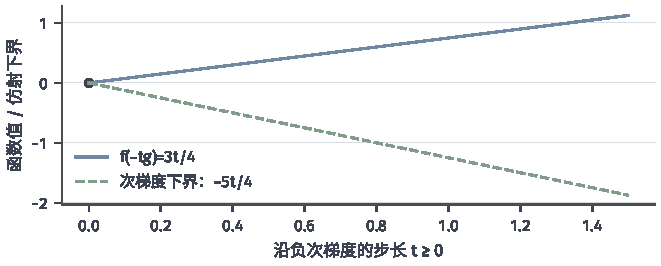
\includegraphics[width=112mm]{figures/00-shared/mathematical-preliminaries-upper/00-shared/matplotlib/mathematical-language-combinatorics-analysis-optimization-comprehension-additions/subgradient-not-descent.pdf}
  \caption{令$f(x,y)=|x|+y/2$、$\bm g=(1,1/2)^\top$。沿$-t\bm g$、$t\geq0$移动时，真实函数值为$3t/4$，该次梯度给出的仿射下界为$-5t/4$。下界始终有效，所选方向却对任意$t>0$上升。}
  \label{fig:vol1-add-subgradient-not-descent}
\end{figure}

再用$f(x,y)=|x|+|y|$检验集合值选择：在$(0.5,0)$处次微分为$\{1\}\times[-1,1]$，选$(1,0)^\top$一步跨到对称点使目标不变；在原点选$(1,1)^\top$则使目标上升。这些反例限定的是逐轮下降保证，总体进展改由历史最佳点或加权平均评价。

\subsection{返回点目标差与预算步长}

设$f$凸、最小点$\bm w^\star$存在、$\|\bm w^{(0)}-\bm w^\star\|_2\leq R$，且实际选出的每个次梯度范数不超过$G$。展开距离平方并用全域支撑，得
\[
 2\eta^{(t)}[f(\bm w^{(t)})-f^\star]
 \leq\|\bm w^{(t)}-\bm w^\star\|_2^2
 -\|\bm w^{(t+1)}-\bm w^\star\|_2^2
 +(\eta^{(t)})^2G^2.
\]
求和后，历史最佳点与步长加权平均点共用目标差界
\begin{equation}
 \min_{t<T}f(\bm w^{(t)})-f^\star
 \leq
 \frac{R^2+G^2\sum_{t<T}(\eta^{(t)})^2}
 {2\sum_{t<T}\eta^{(t)}}.
 \label{eq:opt-subgradient-finite-rate}
\end{equation}
预算$T$已知、$R,G>0$时取$\eta=R/(G\sqrt T)$，两项平衡给$RG/\sqrt T$；这是特定返回点的速率，不是每轮单调下降。预算未知时取$\eta^{(t)}=R/(G\sqrt{t+1})$，累计步长按$\sqrt T$增长、平方步长和按$\log T$增长，给$O(\log T/\sqrt T)$。真正要求的是分母相对初始距离项与平方步长项持续增大；有效定义域、次梯度可选性及有界$G$都须单独核验。实际路径长度为$\sum\eta^{(t)}\|\bm g^{(t)}\|_2$，还含次梯度范数，不能用累计步长代替。

\section{邻近梯度法与邻近点法}

\subsection{邻近算子与可计算的非光滑项}

与其在多个支撑斜率中只挑一条，不如完整保留非光滑项，再加入离中心的平方距离代价，让尖点两侧的形状一起决定走到哪。

\begin{definition}[邻近算子]
\label{def:opt-proximal-operator}
设$r:\mathbb R^d\to\mathbb R\cup\{+\infty\}$适当、下半连续且凸，$\eta>0$。其\term{邻近算子}（proximal operator，近端算子）为
\[
 \operatorname{prox}_{\eta r}(\bm z)
 =\arg\min_{\bm w}\left\{
 r(\bm w)+\frac{1}{2\eta}\lVert\bm w-\bm z\rVert_2^2
 \right\}.
\]
\end{definition}

这里的$\eta$先只是子问题中的权重参数，算法使用它时才成为步长；“闭凸函数”的闭指下半连续，不要求有效定义域本身闭。只最小化$r$可能远离当前点，只最小化距离则不改善$r$，两项平衡给出邻近子问题。

\paragraph{存在唯一与非扩张。}
在适当、下半连续、凸与$\eta>0$条件下，二次距离项是$1/\eta$强凸的。取有限值候选，先可证$r$的负向增长至多线性（在紧球上有下界即可），于是二次项支配远距离，子问题强制且强凸，每个中心有唯一输出。令$\bm p=\operatorname{prox}_{\eta r}(\bm z)$，最优性等价于
\begin{equation}
 \frac{\bm z-\bm p}{\eta}\in\partial r(\bm p),
 \label{eq:opt-prox-optimality}
\end{equation}
故斜率读取于新点。把两个中心$\bm x,\bm y$的最优性不等式相加，得
\begin{equation}
 \lVert\operatorname{prox}_{\eta r}(\bm x)
 -\operatorname{prox}_{\eta r}(\bm y)\rVert_2
 \leq\lVert\bm x-\bm y\rVert_2.
 \label{eq:opt-prox-nonexpansive}
\end{equation}
存在唯一、充要关系和非扩张性不等于子问题能够低成本求解。

\paragraph{软阈值。}
对$r(\bm w)=\lambda\|\bm w\|_1$、$\lambda\geq0$，逐坐标最小化得到\term{软阈值}
\begin{equation}
 [\operatorname{prox}_{\eta r}(\bm z)]_j
 =\operatorname{sign}(z_j)\max\{|z_j|-\eta\lambda,0\}.
 \label{eq:opt-soft-threshold}
\end{equation}
零区间来自子问题最优性所需斜率$z_j/\eta$落在$\lambda[-1,1]$，而不是任取一条次梯度走一步。例如$\bm z=(3,0.4,-2)^\top$与$\eta\lambda=1$输出$(2,0,-1)^\top$；同样输入下二次收缩$z/(1+\eta\lambda)$为$(1.5,0.2,-1)$，二者行为不同。

图~\ref{fig:vol1-add-proximal-balance}画出软阈值所解的完整子问题。
\begin{figure}[!htb]
  \centering
  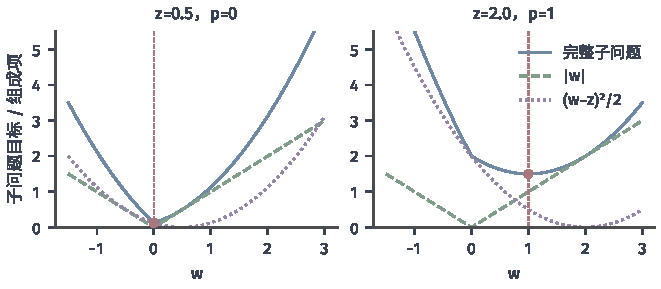
\includegraphics[width=112mm]{figures/00-shared/mathematical-preliminaries-upper/00-shared/matplotlib/mathematical-language-combinatorics-analysis-optimization-comprehension-additions/proximal-balance.pdf}
  \caption{固定$r(w)=|w|$与$\eta=1$，对$z=0.5,2$同时画完整子问题$|w|+(w-z)^2/2$及两项组成。蓝线是完整目标，绿虚线是尖点的$|w|$，紫点线是二次距离。最小点在$0$与$1$，精确最小点的斜率平衡见式~\eqref{eq:opt-prox-optimality}。}
  \label{fig:vol1-add-proximal-balance}
\end{figure}

\subsection{邻近梯度法}

对复合目标$F=f+r$，只对易求梯度的$f$作一阶加二次近似，完整保留$r$，配方后得到
\begin{equation}
 \bm w^{(t+1)}
 =\operatorname{prox}_{\eta r}\!\left(
 \bm w^{(t)}-\eta\nabla f(\bm w^{(t)})\right).
 \label{eq:opt-proximal-gradient-update}
\end{equation}
一轮依次为：在当前有效点求$f$的梯度，形成中心，求$r$的邻近解，核验后接受；回溯试探要重算邻近解。对共同二次目标加$\lambda\|\bm w\|_1$，从$(2,2)$以$\eta=1/16$先到$(15/8,0)$再软阈值，得$(\max\{15/8-\lambda/16,0\},0)$。

\paragraph{原目标下降。}
令$\bm d=\bm w^+-\bm w$，由式~\eqref{eq:opt-prox-optimality}有$-\nabla f(\bm w)-\bm d/\eta\in\partial r(\bm w^+)$。把该支撑不等式用于旧点，再与$f$的光滑上界相加：
\begin{equation}
 F(\bm w^+)\leq F(\bm w)
 -\left(\frac1\eta-\frac L2\right)\|\bm d\|_2^2.
 \label{eq:opt-proximal-gradient-descent}
\end{equation}
此式不要求$f$凸，$0<\eta\leq1/L$即保证下降。未知$L$时增大二次模型系数回溯，域外候选直接拒绝，每次试探都重求邻近解。

\paragraph{梯度映射作为停止量。}
定义可计算的邻近梯度映射
\[
 \bm G_\eta(\bm w)=\frac{\bm w-\bm w^+}{\eta}.
\]
$\bm G_\eta(\bm w)=\bm0$当且仅当$0\in\nabla f(\bm w)+\partial r(\bm w)$，即复合临界条件。属于新点次微分的向量$\bm G_\eta(\bm w)+\nabla f(\bm w^+)-\nabla f(\bm w)$的范数不超过$(1+L\eta)\|\bm G_\eta(\bm w)\|_2$，故旧点映射残差控制新点驻点性。下有界、固定$\eta\leq1/L$时累加式~\eqref{eq:opt-proximal-gradient-descent}给历史最小平方残差$O(1/T)$（范数$O(1/\sqrt T)$）；非凸时这是驻点残差而非全局目标差。

\paragraph{凸复合目标的最后一点目标差。}
再要求$f$凸、最小点存在。旧点凸下界、新点光滑上界与$r$的新点支撑组合成三点不等式
\[
 F(\bm w^+)-F(\bm v)
 \leq\frac{1}{2\eta}\bigl(
 \|\bm w-\bm v\|_2^2-\|\bm w^+-\bm v\|_2^2
 \bigr),
\]
取$\bm v=\bm w^\star$求和，得
\[
 F(\bm w^{(T)})-F^\star
 \leq\frac{\|\bm w^{(0)}-\bm w^\star\|_2^2}{2\eta T}.
\]

\paragraph{固定度量变体。}
若使用11.1.2的固定预条件$\bm P\succ\bm0$，距离项必须匹配：令$\bm z=\bm w-\eta\bm P\nabla f(\bm w)$，子问题为
\[
 \bm w^+=\arg\min_{\bm u}\left\{
 r(\bm u)+\frac{1}{2\eta}\|\bm u-\bm z\|_{\bm P^{-1}}^2
 \right\},\quad
 \|\bm u\|_{\bm P^{-1}}^2=\bm u^\top\bm P^{-1}\bm u.
\]
取$\bm u=\bm P^{1/2}\bm v$即化为欧氏邻近问题；对角$\bm P$与$r=\lambda\|\cdot\|_1$给逐坐标阈值$\eta p_j\lambda$，一般耦合$\bm P$则失去便宜的逐坐标软阈值。只换中心而不换距离，不能沿用欧氏残差界。

\subsection{邻近点法}

若整个目标的邻近问题可解，\term{邻近点法}（proximal point method，近端点法）直接做隐式更新：
\[
 \bm w^{(t+1)}
 =\operatorname{prox}_{\eta^{(t)}F}(\bm w^{(t)}).
\]
每轮固定旧点，组装$F$加距离项，求完整最小点，最优性$(\bm w^{(t)}-\bm w^{(t+1)})/\eta^{(t)}\in\partial F(\bm w^{(t+1)})$中的斜率位于新点。以旧点为可行候选立即得到
\[
 F(\bm w^{(t+1)})
 +\frac{1}{2\eta^{(t)}}\|\bm w^{(t+1)}-\bm w^{(t)}\|_2^2
 \leq F(\bm w^{(t)}).
\]
这里没有由$L$决定的步长上限，但每步可能要求解一个与原问题几乎同样困难的子问题；邻近梯度只线性化$f$正是为减少这一负担。$F$适当闭凸、最小点存在、固定$\eta>0$且子问题精确求解时，最后一点目标差同样为$\|\bm w^{(0)}-\bm w^\star\|_2^2/(2\eta T)$。

\paragraph{弱凸情形的工具边界。}
若原函数$f$为全空间\term{$\rho$弱凸}，即$f+\rho\|\cdot\|_2^2/2$凸，则$\rho>0$时取$0<\eta<1/\rho$，邻近子问题的强凸常数为$1/\eta-\rho$，仍有唯一输出；$\rho=0$时任意正步长适用。但凸邻近的非扩张性不再成立：$f(x)=-\rho x^2/2$的邻近解为$z/(1-\eta\rho)$，反而放大中心扰动。这里建立的只是方法工具的可解性，原$f$有无全局最小点仍由12.6回答。

\section{光滑化逼近法}

当非光滑项具有有限仿射最大值结构、又没有便宜邻近算子时，可以用可控偏差把它替换成光滑函数。固定
\[
 F(\bm w)=\phi(\bm w)+\max_{1\leq i\leq m}\{\bm a_i^\top\bm w+b_i\},
\]
其中$\phi$全空间凸且$L_\phi$光滑。定义$\nu>0$的熵光滑化
\[
 F_\nu(\bm w)=\phi(\bm w)
 +\nu\log\sum_{i=1}^m
 \exp\frac{\bm a_i^\top\bm w+b_i}{\nu}.
\]
把最大仿射值提出指数外，得到全空间一致界
\begin{equation}
 F(\bm w)\leq F_\nu(\bm w)\leq F(\bm w)+\nu\log m.
 \label{eq:opt-smoothing-gap}
\end{equation}
令软权重
\[
 p_i(\bm w)=
 \frac{\exp[(\bm a_i^\top\bm w+b_i)/\nu]}
 {\sum_j\exp[(\bm a_j^\top\bm w+b_j)/\nu]},
\]
则$\nabla F_\nu=\nabla\phi+\sum_i p_i\bm a_i$：这些权重是同一点所有仿射片的软组合，不是原目标的任取次梯度。光滑化最大值的Hessian为权重协方差$\sum_i p_i(\bm a_i-\bar{\bm a})(\bm a_i-\bar{\bm a})^\top$，以$M_A=\max_i\|\bm a_i\|_2$控制得梯度Lipschitz上界$L_\phi+M_A^2/\nu$。减小$\nu$缩小偏差，却增大曲率、缩小可用步长。

给定原目标差要求$\varepsilon$，取$\nu=\varepsilon/(2\log m)$使偏差不超过$\varepsilon/2$，再把光滑求解误差预算设为$\delta\leq\varepsilon/2$。固定$\nu$后可用普通梯度（复杂度$O(\varepsilon^{-2})$）或凸加速程序（$O(\varepsilon^{-1})$）达到$\delta$；一致逼近保证
\[
 F(\widehat{\bm w})-F^\star
 \leq[F_\nu(\widehat{\bm w})-F_\nu^\star]+\nu\log m.
\]
固定$\nu$时增加迭代只减小优化误差、消不去$\nu\log m$；重新减小$\nu$必须重估$L_\nu$，不能沿用旧步长。对$F(x)=|x|$，光滑化为$\nu\log(e^{x/\nu}+e^{-x/\nu})$、梯度为$\tanh(x/\nu)$，跨尖点时实际沿光滑替代更新。这一速度承诺依赖显式最大值结构与全梯度，不适用于任意非光滑黑盒。

\section{束方法}

若凸目标能返回精确函数值与次梯度、却没有易解的邻近算子，单条支撑更新浪费了过去查询揭示的形状。束方法积累全部支撑切面构造下模型，加至稳定中心的距离项求候选，再查原函数决定是否移动中心。

固定$F:\mathbb R^d\to\mathbb R$有限凸，预言器在每个查询点返回精确$F$与$\bm g_j\in\partial F(\bm y_j)$。第$k$轮的束模型为
\[
 m_k(\bm w)=\max_{0\leq j\leq k}
 \{F(\bm y_j)+\bm g_j^\top(\bm w-\bm y_j)\}\leq F(\bm w),
\]
候选由
\[
 \bm y_{k+1}=\arg\min_{\bm w}\left\{
 m_k(\bm w)+\frac{1}{2\tau}\|\bm w-\bm x_k\|_2^2
 \right\}
\]
唯一给出（有限仿射片加正二次项强制且强凸），可用带辅助变量$q$的凸二次规划求解。定义未加二次项的预测下降$\Delta_k=F(\bm x_k)-m_k(\bm y_{k+1})\geq0$；查询$F(\bm y_{k+1})$后，若
\[
 F(\bm x_k)-F(\bm y_{k+1})\geq\beta\Delta_k
\]
则接受为实质步、移动稳定中心，否则为空步、中心不变；两种情况都把新切面加入束。空步消耗查询并改进模型，却不移动中心。

令$\bm s_k=(\bm x_k-\bm y_{k+1})/\tau$，模型最优性与中心处模型精确性推出带误差支撑
\[
 F(\bm w)\geq F(\bm x_k)+\bm s_k^\top(\bm w-\bm x_k)-e_k,
 \qquad e_k=\Delta_k-\tau\|\bm s_k\|_2^2\geq0.
\]
若已知某最小点满足$\|\bm x_k-\bm w^\star\|\leq R_k$，则$F(\bm x_k)-F^\star\leq e_k+R_k\|\bm s_k\|_2$，可作停止证书；$\Delta_k=0$给出精确全局最优，$\Delta_k$小本身不等于目标差。在全空间$M$-Lipschitz、固定参数和有界中心距离等条件下，全记忆邻近束方法让$\varepsilon\downarrow0$时实质步数为$O(\varepsilon^{-1})$、空步数为$O(\varepsilon^{-3})$；不能剔除空步后宣称总查询数为$O(\varepsilon^{-1})$，一次外层计数也不含模型二次规划的内迭代。

\section{原目标最小解的存在唯一与最优性}

\subsection{最小值是否达到、最小点是否唯一}

非光滑本身既不提供紧性，也不保证下确界有限或达到，存在性仍用第10章的条件：$F$适当、下半连续且某有限下水平集非空紧（强制性是常用充分条件）时最小点达到。凸性不能替代这两步：$F(x,y)=e^x+|y|$下确界为$0$却没有最小点；$F(x,y)=|x|$的最小点是整条直线$x=0$。严格凸只保证至多一个最小点；适当闭的全空间$\mu$强凸目标可用二次项的增长得到强制性与唯一最小点，$F(x)=|x|+\mu x^2/2$就是非光滑而唯一可解的例子。这里用的是原目标曲率，邻近子问题的唯一解不能代替它。

\subsection{候选点的全局最优与局部驻点}

\subsubsection{凸支撑证书}

对有限值点，$\bm0\in\partial f(\bm w^\star)$与全局最小性等价：把零向量代入支撑不等式直接得$f(\bm v)\geq f(\bm w^\star)$；反方向由全局最小性得零向量是次梯度。注意判据要求“零向量属于次微分”，不要求次微分只有零向量，也不要求算法任选的次梯度为零。这一证明依赖全域支撑定义。

\subsubsection{Clarke局部信息与必要条件}

失去凸支撑后，只能改问局部极小点必须满足什么斜率条件。

\paragraph{邻近梯度极限与移动基点。}
对开集$U\subseteq\mathbb R^d$上的局部Lipschitz函数，收集邻近可微点梯度沿趋于当前点序列的全部极限，取闭凸包，定义\term{Clarke广义梯度}（Clarke generalized gradient）$\partial^\circ f(\bm x)$；可微点足够丰富的依据是Rademacher定理（局部Lipschitz函数几乎处处可微），不能由逐坐标切片直接推出多元结论。允许起点也移动的方向导数为
\[
 f^\circ(\bm x;\bm v)
 =\limsup_{\bm y\to\bm x,\ t\downarrow0}
 \frac{f(\bm y+t\bm v)-f(\bm y)}{t},
\]
并有等价刻画
\[
 \partial^\circ f(\bm x)
 =\{\bm g:\bm g^\top\bm v\leq f^\circ(\bm x;\bm v),\ \forall\bm v\}.
\]
对$C^1$函数该集合退化为单个梯度；仅当前点可微不足以保证退化。一元情形中，$f^\circ(x;v)$可用缩小邻域上的上确界定义，局部Lipschitz保证差商有限。

在$|x|$与$-|x|$的零点，两侧导数交换次序却产生同一个$[-1,1]$；多元例$f(x,y)=\pm|x|$在$x=0$给$[-1,1]\times\{0\}$。

图~\ref{fig:analysis-clarke-stationarity-boundary}用同一候选斜率比较两个函数。
\begin{figure*}[htbp]
  \centering
  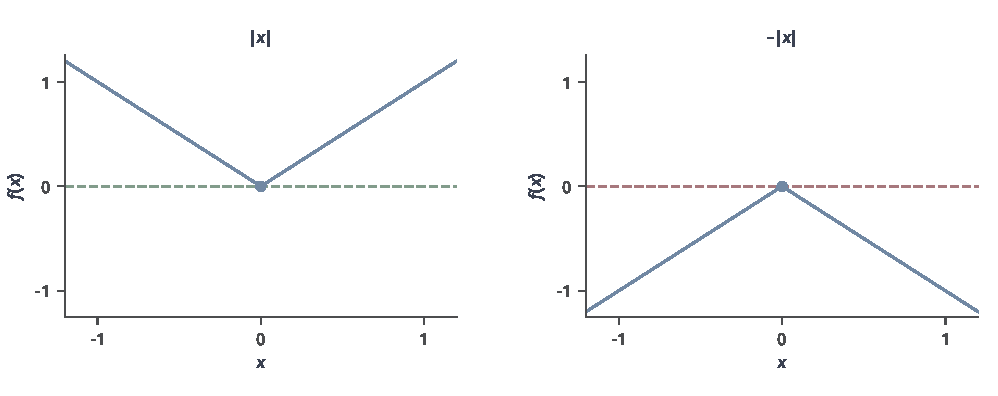
\includegraphics[width=169.0mm]{figures/00-shared/mathematical-preliminaries-upper/04-optimization/matplotlib/analysis-clarke-stationarity-boundary/figure.pdf}
  \caption{同一广义梯度区间$[-1,1]$的两种含义。蓝线分别为$|x|$与$-|x|$，虚线为原点候选斜率$g=0$的直线。左图候选直线在全局下界，右图原函数处处在直线下方。两图在原点都满足$0\in\partial^\circ f$，却分别是局部最小点和局部最大点。}
  \label{fig:analysis-clarke-stationarity-boundary}
\end{figure*}

\paragraph{含零必要性与最小性边界。}
局部极小点处，在移动基点差商中取固定基点$\bm y=\bm x$，所有足够小正$t$的分子非负，故$f^\circ(\bm x;\bm v)\geq0$对全部$\bm v$成立，由等价刻画得$0\in\partial^\circ f(\bm x)$，这是必要条件。反方向不成立：$-|x|$在原点是局部最大点而Clarke集合含零；若要求全域仿射下界，正半轴迫使$g\leq-1$、负半轴迫使$g\geq1$，斜率集合为空。局部Lipschitz凸函数的Clarke集合与凸次微分一致——只有恢复凸结构，才能引用12.6.2.1的全局判据。

\subsection{曲率条件不能互相替换}

用同一族二次函数隔离曲率条件的差别：
\[
 f_a(x_1,x_2)=\frac12(x_1+x_2)^2+\frac a2(x_1-x_2)^2.
\]
$a>0$时强凸；$a=0$时凸、满足PL但最小点成直线；$a<0$时弱凸而无下界。$f(x)=\cos x$二阶导数下界为$-1$，故为$1$弱凸却有无穷多个低点，在$x=0$梯度为零而目标差为$2$，没有正PL常数；前文的$f(x,y)=x^2+2\sin^2x$说明PL与弱凸可以共存。弱凸只限制可被二次距离补偿的负曲率，不保证全局最优、驻点唯一或收敛速度。

\begin{table*}[htbp]
 \centering\small
 \begin{tabularx}{\linewidth}{@{}lXX@{}}
 \toprule
 条件 & 直接控制什么 & 单凭该条件不能得到什么 \\
 \midrule
 凸性 & 全部线段上的弦上界；局部最小点也是全局最小点 & 最小点存在、最小点唯一或统一收敛速率 \\
 严格凸性 & 非平凡线段上的严格不等式；最小点至多一个 & 最小点存在，例$e^x$无最小点 \\
 强凸性 & 弦段与函数的二次间隔；目标差$\geq$距离平方界 & 梯度光滑性；例$|x|+\mu x^2/2$仍有尖点 \\
 弱凸性 & 最坏负曲率的可补偿下界 & 驻点全局最优或最小点唯一；$\cos x$有多个低点 \\
 PL条件 & 梯度平方控制目标差 & 凸性或参数唯一；可有多解与非凸景观 \\
 \bottomrule
 \end{tabularx}
 \caption{曲率条件的职责比较。各行针对不同性质，不能排成一条从“弱”到“强”的完整等级。}
 \label{tab:opt-curvature-conditions}
\end{table*}

\section{原问题的收敛速度与精度}

\subsection{原目标差与实际返回点}

凸问题、最小点存在且次梯度有界时，历史最佳点或加权平均点给$O(T^{-1/2})$目标差（预算未知的步长例多一对数因子）。精确邻近点法与凸邻近梯度法在各自精确子问题和合格步长下给最后一点$O(T^{-1})$，但一次调用是子问题而非一次廉价梯度读取。光滑化把原目标差拆成光滑优化误差与固定偏差$\nu\log m$；束方法以模型误差与到解距离控制中心。比较的是原目标误差与实际返回对象，阶数高不代表所有迭代点都更接近参数解。

\subsection{临界残差与全局目标差的边界}

光滑项失去凸性、非光滑项仍闭凸时，邻近梯度的历史最小平方梯度映射为$O(T^{-1})$（范数$O(T^{-1})$平方根即$O(T^{-1/2})$）；它控制复合临界性，不直接给最小值差，Clarke含零也只有必要性。目标差趋零、临界残差趋零、参数接近最小点是三件事，相互转换需要增长或误差界结构。

\subsection{预言器、子问题与精度预算}

复杂度先固定精度口径与计数单位：次梯度法的$O(\varepsilon^{-2})$是支撑读取数；精确邻近方法的$O(\varepsilon^{-1})$是子问题调用数；显式最大值的光滑化在统一距离界下普通／加速求解分别给$O(\varepsilon^{-2})$、$O(\varepsilon^{-1})$全梯度预算，还要按精度重选$\nu$与$L_\nu$；束方法既计实质步也计空步和随记忆增长的二次规划成本。这些阶数跨信息模型不能直接排序；不精确信息先按第14章明确误差来源与工作量。

\section{迭代过程与数值敏感度}

\subsection{原目标是否逐步改善}

\subsubsection{支撑更新不保证逐步下降}

12.2.3的三组反例——跨过尖点的大步、任意小步仍上升的负次梯度方向、尖点处不同支撑选择——共同否定逐轮下降推断。次梯度法的总体进展只能按历史最佳点或加权平均评价。

\subsubsection{由原目标比较保证的非增更新}

精确完整邻近点更新以旧点为候选，直接保证原目标非增并为位移付出正平方代价；精确邻近梯度在合格步长下由光滑上界与凸支撑使原复合目标非增，光滑项不凸也成立；束方法的实质步检验原$F$至少减少$\beta\Delta_k$，空步保持中心目标，查询点目标则可以上升。比较时要同时记录中心与查询点。

\subsubsection{只控制替代目标的光滑化更新}

普通梯度步在合格步长下使固定$F_\nu$下降，不能据此声称$F$逐步下降；加速更新甚至不承诺$F_\nu$逐步单调。应同时记录光滑替代值与原目标值，按两项误差界判断最终输出。

\subsection{目标进展能否推出参数收敛}

固定正步长、精确邻近更新且目标下有界时，累加下降式得平方位移可和、位移趋零，但这不证明路径总长度有限，也不单独给全序列收敛。在凸条件、固定步长与精确计算下，邻近比较使到任一原最小点的距离非增；目标差趋零配合有限维有界子列与闭目标，聚点落入解集，再由距离极限得全序列趋于其中一个解。多解时初值与规则可能选择不同解；次梯度法的最佳点或平均点界只评价返回序列。

\subsection{原解变化与计算扰动}

数据或正则参数改变时，首先比较两个原目标的最小点：适当闭$\mu$强凸$F$的线性扰动给$\|\bm w_{\bm b}-\bm w_{\bm c}\|_2\leq\|\bm b-\bm c\|_2/\mu$，不要求可微，但缺少原目标曲率时不能从邻近子问题唯一性推出此界。固定$r,\eta$时凸邻近映射非扩张只控制一次调用的中心误差；弱凸邻近输出可能放大误差；次梯度在尖点的不同选择可形成不同轨迹。原问题解集、一次调用与多步轨迹是三个对象，一般多步传播回用11.5的扩展状态框架。

\section{本章小结}

尖点处有四条求解路线：次梯度法读取一条全域支撑，邻近梯度法保留可求邻近的非光滑项，光滑化法用受控偏差取得单个光滑梯度，束方法积累下模型并核验原目标改善；邻近点法说明完整子问题的隐式更新。每步成本、是否逐步下降及最终返回对象都分别报告。

在原问题层面，存在性需要紧性或增长条件，唯一性需要原目标的额外结构；凸次微分含零给全局最优，Clarke含零一般只有必要性。目标差、平方驻点残差与参数收敛各有条件和评价对象。下一章中，指标函数的邻近映射将成为闭凸集投影，非光滑罚函数可调用本章方法，但原约束的可行性仍须独立检查。

\chapter{有约束优化的求解}
\label{chap:constrained-optimization}

目标下降的一步可能越过资源边界。本章固定原问题
\[
 \min_{\bm w\in C}f(\bm w),\qquad
 C=\{\bm w:\ a_j(\bm w)=0\ (j=1,\ldots,m),\ g_k(\bm w)\leq0\ (k=1,\ldots,p)\},
\]
比较三类约束处理：投影直接选择域内最近点，惩罚把违反量加入目标，乘子把每条约束的影响写成待定系数。三种机制可以组合，但改变的计算对象不同；而且投影可行不证明目标已足够好，罚目标改善不保证原约束满足，Lagrangian内层点也可能不可行。共同二次目标加等式$w_1+w_2=1$贯穿法向、罚参数与乘子平衡，非负预算分配贯穿活跃集、对偶更新与敏感性。

\section{约束表示与核验对象}

\subsection{原问题与可行域}

变量为$\bm w\in\mathbb R^d$，等式$a_j(\bm w)=0$、不等式$g_k(\bm w)\leq0$共同确定$C$；调用梯度时另要求目标与约束在所用邻域可微。能否保持可行、能否找到可行点、可行点的目标质量是三个不同问题。

\subsection{乘子、KKT关系与局部残差}

可行点处$g_k(\bm w)=0$称为约束活跃。满足
\[
 \langle\nabla a_j(\bm w),\bm d\rangle=0,\qquad
 \langle\nabla g_k(\bm w),\bm d\rangle\leq0
\]
（等式取全部、不等式取活跃集）的方向称为\term{线性化可行方向}；它是一阶近似，不保证$t\bm d$是真实可行位移。定义\term{拉格朗日函数}（Lagrangian）
\begin{equation}
 \mathcal L(\bm w,\bm\nu,\bm\alpha)
 =f(\bm w)+\sum_j\nu_j a_j(\bm w)+\sum_k\alpha_k g_k(\bm w),
 \qquad
 \bm\nu\in\mathbb R^m,\ \bm\alpha\geq\bm0.
 \label{eq:opt-lagrangian}
\end{equation}

\paragraph{四组KKT条件及其含义。}
\term{Karush--Kuhn--Tucker条件}（KKT条件）要求候选同时满足：驻点性$\nabla_{\bm w}\mathcal L=\bm0$；原始可行性$a_j=0$、$g_k\leq0$；对偶可行性$\alpha_k\geq0$（等式乘子无符号限制）；逐项互补松弛$\alpha_k g_k=0$。四组条件分别对应目标梯度被法向抵消、候选满足原始限制、价格符号非负、“卡住才标价”。由互补松弛知严格松弛的约束乘子为零、正乘子约束必活跃；但活跃约束仍可有零乘子。全部等式与活跃不等式梯度线性无关称为LICQ。数值计算应分开报告驻点范数、等式残差、不等式正部、负乘子正部和互补乘积，它们是候选核验量，脱离尺度不自动给目标差。

\subsection{对偶函数、上下界与全局间隙}

固定$\bm\nu\in\mathbb R^m$、$\bm\alpha\geq\bm0$，对原始可行点，等式项为零、不等式项非正，故$\mathcal L\leq f$。定义\term{对偶函数}与两个极值
\[
 q(\bm\nu,\bm\alpha)=\inf_{\bm w}\mathcal L(\bm w,\bm\nu,\bm\alpha),\qquad
 p^\star=\inf_{\bm w\in C}f(\bm w),\quad
 d^\star=\sup_{\bm\nu,\bm\alpha\geq\bm0}q(\bm\nu,\bm\alpha).
\]
用下确界和上确界表述，不预设达到。由构造有$d^\star\leq p^\star$，称为\term{弱对偶}；两值有限时差$p^\star-d^\star$为对偶间隙。某组乘子给$q=-\infty$是一个候选无有限下界，对偶可行域为空是整个候选集合问题，不能混用。

若$\widehat{\bm w}$原始可行且$L=q(\bm\nu,\bm\alpha)$有限，则
\begin{equation}
 L\leq p^\star\leq U=f(\widehat{\bm w}),\qquad
 0\leq U-p^\star\leq U-L.
 \label{eq:opt-duality-certificate}
\end{equation}
可行候选给上界、对偶值给下界，两者间隔才是停止证书；求$q$时的内层点若不可行，不能充当$U$。

\section{投影梯度法}

\subsection{投影对象与可计算的距离子问题}

对非空闭凸集$C$定义欧氏\term{投影}
\begin{equation}
 \Pi_C(\bm z)=\arg\min_{\bm w\in C}\lVert\bm w-\bm z\rVert_2^2.
 \label{eq:opt-projection}
\end{equation}
因$\iota_C$适当、下半连续且凸，投影正是$\operatorname{prox}_{\eta\iota_C}$（比例因子不改变最小点），存在唯一性直接复用邻近算子结论。

\begin{proof}[最近点的存在唯一与法向不等式]
任取$\bm x_0\in C$，只在$C\cap\{\bm x:\|\bm x-\bm z\|\leq\|\bm x_0-\bm z\|\}$这个非空紧集上考虑，连续距离在此达到最小。若$\bm p_1,\bm p_2$都是最近点，凸性给中点$\bm p\in C$，由平行四边形恒等式
\[
 \|\bm z-\bm p\|_2^2
 =\frac12\|\bm z-\bm p_1\|_2^2+\frac12\|\bm z-\bm p_2\|_2^2
 -\frac14\|\bm p_1-\bm p_2\|_2^2,
\]
两点相异就会严格小于最近距离平方，矛盾，故唯一。对任意$t\in[0,1]$，$\bm p+t(\bm x-\bm p)\in C$，函数$q(t)=\|\bm z-[\bm p+t(\bm x-\bm p)]\|^2$在$t=0$最小，右导数非负给出法向不等式
\begin{equation}
 \langle\bm z-\bm p,\bm x-\bm p\rangle\leq0
 \quad\text{对所有 }\bm x\in C.
 \label{eq:opt-projection-normal}
\end{equation}
展开即得投影不增加到任一可行参照点的距离：
\begin{equation}
 \|\bm p-\bm x\|_2^2+\|\bm z-\bm p\|_2^2\leq\|\bm z-\bm x\|_2^2.
 \label{eq:opt-projection-distance}
\end{equation}
\end{proof}

图~\ref{fig:vol1-add-projection-normal}把$\bm z-\bm p$与可行弦画在同一起点。
\begin{figure}[!htb]
  \centering
  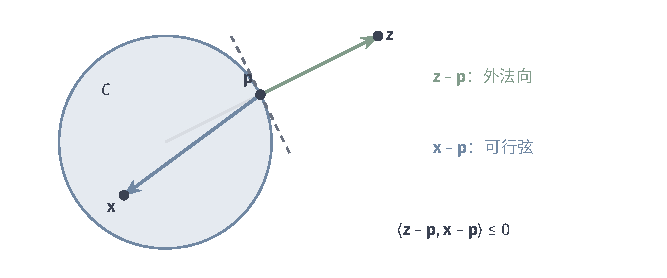
\includegraphics[width=112mm]{figures/00-shared/mathematical-preliminaries-upper/00-shared/tikz/mathematical-language-combinatorics-analysis-optimization-comprehension-additions/projection-normal.pdf}
  \caption{取闭单位圆盘$C$、外点$\bm z=(2,1)^\top$，投影为$\bm p=\bm z/\|\bm z\|_2$。绿箭头$\bm z-\bm p$沿外法向，蓝箭头$\bm x-\bm p$是任一可行弦，内积$\langle\bm z-\bm p,\bm x-\bm p\rangle\leq0$。图中一个参照点仅用于展示。}
  \label{fig:vol1-add-projection-normal}
\end{figure}

盒约束投影逐坐标截断，成本$O(d)$。概率单纯形$\Delta=\{\bm w:w_j\geq0,\sum_jw_j=1\}$不能逐坐标截断，其投影具有共同阈值形式$p_j=\max\{z_j-\tau,0\}$：先排序，再确定正坐标集合，由总和定$\tau$，常用实现$O(d\log d)$。一般凸集的投影本身可能是昂贵子问题。

\subsection{欧氏投影梯度的更新与实现}

把光滑一阶模型加欧氏距离项、只在$C$内最小化，配方得到
\begin{equation}
 \bm w^{(t+1)}
 =\Pi_C\!\left(\bm w^{(t)}-\eta^{(t)}\nabla f(\bm w^{(t)})\right).
 \label{eq:opt-projected-gradient}
\end{equation}
从可行初值出发，输出恒属于$C$。在包含候选与比较线段的开凸域上要求$f$为$L$光滑、取$0<\eta\leq1/L$；未知$L$时按光滑上界回溯，试探要重新求投影。停止量为
\[
 \frac{\|\bm w-\Pi_C(\bm w-\eta\nabla f(\bm w))\|_2}{\eta}
\]
连同原始可行性一起核验。在共同二次目标上取$C=[1,2]\times[0,2]$，$\eta=0.1$时第一步先到梯度中心$(1.8,-1.2)$再投影为$(1.8,0)$；约束最小点$(1,0)$的普通梯度为$(1,0)\neq\bm0$。

\subsection{固定度量的投影梯度变体}

与固定预条件$\bm P\succ\bm0$组合时，投影要匹配距离：
\[
 \bm w^+=\arg\min_{\bm u\in C}
 \|\bm u-(\bm w-\eta\bm P\nabla f(\bm w))\|_{\bm P^{-1}}^2.
\]
其固定点条件消去$\bm P^{-1}\bm P$后恢复原问题的可行一阶条件；若误用欧氏投影截回预条件中心，固定点一般变成$\langle\bm P\nabla f(\bm w),\bm u-\bm w\rangle\geq0$，不等于原条件。对角$\bm P$加盒约束仍逐坐标可分，单纯形或一般耦合$\bm P$须求解新加权最近点问题，不能按原投影成本计费。

\subsection{边界停止与原始目标差}

由式~\eqref{eq:opt-projection-normal}，投影固定点等价于可行一阶条件
\[
 \langle\nabla f(\bm w),\bm v-\bm w\rangle\geq0
 \quad\text{对所有 }\bm v\in C.
\]
若$f$凸，一阶凸下界使该条件足以给原域全局最优；非凸时它只是可行一阶条件。凸$L$光滑、最小点存在、$0<\eta\leq1/L$时，邻近梯度的三点不等式直接给投影迭代目标差$O(1/T)$。

投影梯度与前两章的一阶更新形式相近，但它们把结构放进更新的不同位置。表~\ref{tab:opt-first-order-structures}统一比较每一步实际处理的对象；表中的条件只说明调用相应分析前要核对什么，不把四种方法归入同一条收敛定理。

\begin{table*}[!htb]
 \centering\small
 \begin{tabularx}{\linewidth}{@{}lXX@{}}
 \toprule
 更新方式 & 每步处理的结构 & 分析前需核对的条件\\
 \midrule
 梯度下降 & 使用可微目标的梯度 & 光滑常数与步长；全局最优保证还依赖凸性或PL等条件\\
 投影梯度 & 梯度更新后求可行集最近点 & 非空闭凸集；投影本身的计算成本\\
 次梯度更新 & 使用非光滑凸目标的全局下界斜率 & 次梯度范数及步长序列；单步目标未必下降\\
 近端梯度 & 光滑部分求梯度，非光滑部分求邻近解 & 光滑部分的步长、正则项的适当闭凸性及可解邻近子问题\\
 \bottomrule
 \end{tabularx}
 \caption{常见一阶更新的结构与条件。相近的更新形式并不共享同一收敛定理。}
 \label{tab:opt-first-order-structures}
\end{table*}

\subsection{梯度与投影误差的传播}

精确映射$T_t(\bm w)=\Pi_C(\bm w-\eta_t\nabla f(\bm w))$；实际梯度读数为$\nabla f(\widetilde{\bm w}^t)+\bm e_t$，含误差中心的精确投影为$\bm p_t$，实际输出满足$\|\widetilde{\bm w}^{t+1}-\bm p_t\|\leq\zeta_t$。投影非扩张给
\[
 \delta_{t+1}\leq\rho_t\delta_t+\eta_t\|\bm e_t\|+\zeta_t,
\]
其中仅$L$光滑时可取$\rho_t=1+\eta_t L$；凸且$L$光滑、$0<\eta_t\leq2/L$时取$1$；再加强凸与$0<\eta_t\leq1/L$时可取$1-\eta_t\mu$。距离误差$\zeta_t$不自动保证输出严格属于$C$，须同时检查实际可行性；实际停止读数与真实投影梯度映射之差不超过$\|\bm e_t\|+\zeta_t/\eta_t$，步长很小时会放大投影计算误差。

\section{惩罚法}

投影难求时，可以允许暂时不可行，把违反量折算进目标。

\subsection{二次惩罚法}

\subsubsection{构造与内外层执行}

二次惩罚目标为
\[
 f+\frac{\rho}{2}\left(\sum_j a_j^2+\sum_k[g_k]_+^2\right).
\]
$[t]_+^2$的导数为$2[t]_+$，故在$f$与约束连续可微时罚项连续可微；约束仿射时还凸且梯度Lipschitz，一般非线性约束（如$a(x)=x^2-1$的平方$(x^2-1)^2$）两项都不继承。执行时先固定$\rho$，核验罚目标结构并选第11—12章的求解器，内层分别报告原目标、违反量与求解精度；外层逐步增大$\rho$，不能仅凭罚目标小梯度停机。

\subsubsection{可行极限与罚参数代价}

对共同目标加等式$w_1+w_2=1$，解驻点方程得
\[
 \bm w_\rho=\frac{(16\rho,\rho)^\top}{16+17\rho},\qquad
 w_1+w_2-1=-\frac{16}{16+17\rho}.
\]
任何有限$\rho>0$仍不可行，极限才是$(16/17,1/17)$。罚Hessian为$\operatorname{diag}(1,16)+\rho\bm1\bm1^\top$，最大特征值随$\rho$趋于无穷，固定步长上限$2/\lambda_{\max}$缩小；最小特征值从$1$增至$17/2$，条件数并非单调变化（$\rho=0,1,225/34$各阶段方向不同），不能只凭最大曲率增大断言持续恶化。

图~\ref{fig:vol1-add-penalty-feasibility-curvature}的两个解析分面分别衡量残差和曲率。
\begin{figure*}[htbp]
  \centering
  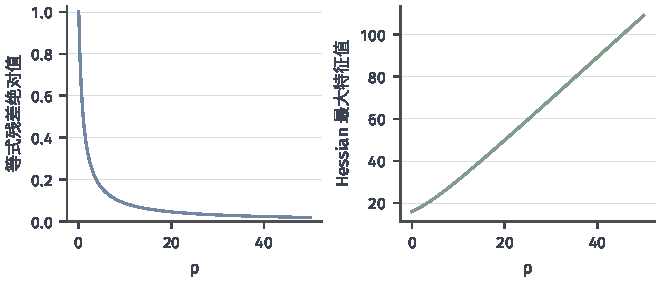
\includegraphics[width=169.0mm]{figures/00-shared/mathematical-preliminaries-upper/00-shared/matplotlib/mathematical-language-combinatorics-analysis-optimization-comprehension-additions/penalty-feasibility-curvature.pdf}
  \caption{共同二次等式加二次惩罚的解析结果。左图约束违反量$16/(16+17\rho)$随$\rho$趋零；右图罚Hessian最大特征值$(17+\sqrt{225+4\rho^2})/2$随$\rho$增大。两图分别衡量可行性与曲率代价，最大特征值不等于条件数。}
  \label{fig:vol1-add-penalty-feasibility-curvature}
\end{figure*}

极限结论需要三个条件各管一段：设违反量$P\geq0$连续、$P=0$恰表可行，$f$下半连续且在候选区域有统一下界$m$，存在可行$\bar{\bm w}$，$\bm w_\rho$精确最小化$f+\rho P$，则与$\bar{\bm w}$比较给$\rho P(\bm w_\rho)\leq f(\bar{\bm w})-m$，违反量随$\rho\to\infty$趋零；再有有界子列才取得极限点；由$P$连续得极限可行，再与任意可行点比较、用下半连续性得极限全局最优。内层近似求解（次优差$\varepsilon_\rho$）时违反量趋零需$\varepsilon_\rho/\rho\to0$。

\subsection{精确惩罚法}

绝对残差
\begin{equation}
 V(\bm w)=\sum_j|a_j(\bm w)|+\sum_k[g_k(\bm w)]_+
 \label{eq:opt-exact-penalty}
\end{equation}
在约束成立时恰为零，罚目标$f+\rho V$通常非光滑，可用第12章的次梯度或邻近方法（但$|a_j(\bm w)|$一般不能逐坐标软阈值）。有限$\rho$能保持原最小解，有两种独立依据。

\paragraph{由可行修复误差界。}
设比较区域$D$含候选及其可行修复，$f$在$D$上$K$-Lipschitz，每个$\bm w\in D$有可行$\bm p\in D$使$\|\bm p-\bm w\|_2\leq\kappa V(\bm w)$，则
\[
 f(\bm w)+\rho V(\bm w)
 \geq f(\bm p)+(\rho-K\kappa)V(\bm w).
\]
$\rho>K\kappa$时不可行点严格劣于其修复点，区域内罚最优解必可行。

\paragraph{由达到的最优乘子。}
若凸约束问题原、对偶均达到且零间隙，取$\rho>\max\{\|\bm\nu^\star\|_\infty,\|\bm\alpha^\star\|_\infty\}$，绝对／正部罚项不小于最优Lagrangian，并对任何非零违反多出严格正量。共同等式例$\nu^\star=-16/17$，故$\rho>16/17$的绝对值惩罚已经精确，与二次惩罚只能在极限可行形成对照。

\subsection{范数惩罚与硬范围的解对应}

硬约束$\|\bm w\|_1\leq R$规定允许范围，正则项$\lambda\|\bm w\|_1$按规模计价，二者不同。若原问题有原始最优解、强对偶成立且有限乘子$\lambda^\star$达到，则原最优解同时最小化$f+\lambda^\star\|\bm w\|_1$（常数$-\lambda^\star R$不改变最小点）；仅有值相等不保证乘子存在。反方向，若$\widehat{\bm w}$最小化$f+\lambda\|\cdot\|_1$，令$R=\|\widehat{\bm w}\|_1$，它也最小化半径$R$的约束问题，但这只构造匹配半径，不证明$\lambda$与$R$一一对应，非凸时还可能有对偶间隙。普通欧氏GD下$f+\lambda\|\bm w\|_2^2/2$的更新为$(1-\eta\lambda)\bm w-\eta\nabla f$；加预条件$\bm P$后正则项走$-\eta\lambda\bm P\bm w$，与独立衰减$-\eta\lambda\bm w$只在匹配条件下相同。

图~\ref{fig:opt-proximal-comparison}比较同一标量输入下投影、软阈值与二次收缩。
\begin{figure}[!htb]
  \centering
  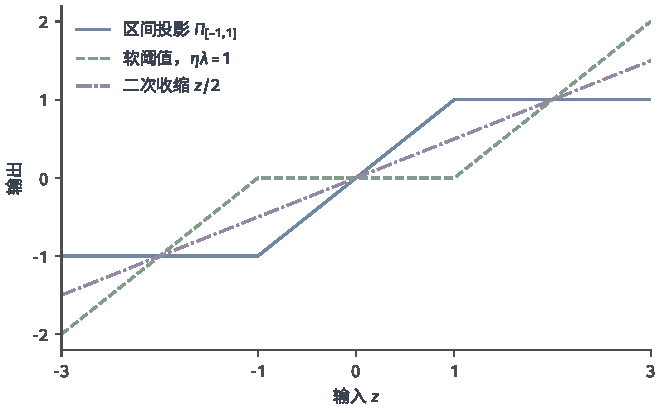
\includegraphics[width=112.0mm]{figures/00-shared/mathematical-preliminaries-upper/04-optimization/matplotlib/opt-proximal-comparison/figure.pdf}
  \caption{同一输入$z$的三种邻近映射。区间投影把值截到边界，软阈值把小幅值置零，二次惩罚按比例缩小。}
  \label{fig:opt-proximal-comparison}
\end{figure}

\section{投影对偶上升法}

\subsection{内层求解与乘子更新}

合记乘子$\bm y=(\bm\nu,\bm\alpha)$、允许域$Y=\mathbb R^m\times\mathbb R_+^p$。每轮固定乘子求Lagrangian内层最小点，以约束残差更新价格：
\begin{equation}
 \begin{aligned}
 \bm w^{(t)}&\in\arg\min_{\bm w}\mathcal L(\bm w,\bm y^{(t)}),\\
 \bm s^{(t)}&=(\bm a(\bm w^{(t)}),\bm g(\bm w^{(t)})),\\
 \bm y^{(t+1)}&=\Pi_Y(\bm y^{(t)}+\eta^{(t)}\bm s^{(t)}).
 \end{aligned}
 \label{eq:opt-dual-ascent}
\end{equation}
等式乘子直接加残差，不等式乘子截到非负；违反预算使价格上升，有余量使价格下降。先完整取得内层输出再更新乘子，新旧乘子不能混用。

\subsection{残差方向、步长与对偶目标差}

对任意$\bm y'\in Y$，把当前内层点代入有
\[
 q(\bm y')\leq q(\bm y^{(t)})
 +\langle\bm s^{(t)},\bm y'-\bm y^{(t)}\rangle,
\]
即$q$凹、残差是其全局仿射上界斜率，更新等价于对凸函数$-q$作投影次梯度下降。在最优乘子存在、初始距离$\leq R_y$、残差范数$\leq G_y$下，
\[
 d^\star-\max_{t<T}q(\bm y^{(t)})
 \leq\frac{R_y^2+G_y^2\sum_{t<T}(\eta^{(t)})^2}
 {2\sum_{t<T}\eta^{(t)}},
\]
常步长$\eta=R_y/(G_y\sqrt T)$给$R_yG_y/\sqrt T$。它控制已访问下界，不保证每轮$q$上升，也不控制内层点可行性。

若固定闭凸域上$f$为$\mu$强凸、约束仿射为$\bm A\bm w-\bm b$且内层唯一解达到，则$\bm w(\bm y)$是Lipschitz映射（常数$\|\bm A\|_2/\mu$），两组内层解夹住$q$的增量可证$q$可微且
\[
 \nabla q(\bm y)=\bm A\bm w(\bm y)-\bm b,\qquad
 L_q=\|\bm A\|_2^2/\mu,
\]
从而回用投影梯度的$O(1/T)$光滑界；$\bm A=\bm0$时梯度恒定，取任意正上界。一般非线性约束或多解内层不能直接套用。

\subsection{近似内层的执行、误差与可信下界}

近似内层点须有可信证书$\mathcal L(\widetilde{\bm w}^{(t)},\bm y^{(t)})\leq q(\bm y^{(t)})+\epsilon^{(t)}$；只用其残差更新时，仿射上界多出$\epsilon^{(t)}$，累计目标差界分子增加$2\sum_t\eta^{(t)}\epsilon^{(t)}$，且必须对实际参与更新的近似残差核验有界。近似内层值本身在$q$上方，可信下界应为
\[
 \mathcal L(\widetilde{\bm w}^{(t)},\bm y^{(t)})-\epsilon^{(t)}\leq q(\bm y^{(t)}),
\]
不能直接把内层值充作原问题下界。

\subsection{原始可行恢复与上下界证书}

在预算例（固定$\tau=2$，只对总预算设乘子）中，内层解$\bm w(\alpha)=((2-\alpha)_+,(1-\alpha)_+)^\top$，$q(\alpha)=\alpha-\alpha^2$；取$\alpha^{(0)}=0$、$\eta=1/4$，有$\alpha^{(t)}=\frac12(1-2^{-t})$，前三轮内层点$(2,1),(7/4,3/4),(13/8,5/8)$全部超预算，违反量为$1,1/2,1/4$，而$q$趋于$1/4$。本例两坐标恒正，各减一半预算残差即修复为$(3/2,1/2)$、$U=1/4$；这种简单恢复依赖本例结构，一般问题需独立的投影或恢复算法。即使乘子最优，任意内层点也未必是原解：资源LP对偶例的最优价格处Lagrangian对所有非负分配同值，选$(10,10)$不可行、选$(0,0)$可行却非最优。

\section{对偶分解法}

\subsection{复制变量与独立内层}

对$\min_{\bm w}\{r(\bm w)+s(\bm w)\}$引入两个副本，改写为
\[
 \min_{\bm u=\bm v}\{r(\bm u)+s(\bm v)\}.
\]
一致性等式使两题可行目标相同，复制只改变计算位置。固定等式乘子$\bm\nu$，两个内层独立求解：
\begin{equation}
 \begin{aligned}
 \bm u^{(t)}&\in\arg\min_{\bm u}\{r(\bm u)+\langle\bm\nu^{(t)},\bm u\rangle\},\\
 \bm v^{(t)}&\in\arg\min_{\bm v}\{s(\bm v)-\langle\bm\nu^{(t)},\bm v\rangle\},\\
 \bm\nu^{(t+1)}&=\bm\nu^{(t)}+\eta^{(t)}(\bm u^{(t)}-\bm v^{(t)}).
 \end{aligned}
 \label{eq:opt-consensus-dual-decomposition}
\end{equation}
取齐本轮副本后才算残差、更新乘子；局部副本可暂时不一致，改进的是对偶下界，原目标不保证逐轮下降。

\subsection{强凸与仅凸内层的步长依据}

若$r,s$分别为$\mu_r,\mu_s$强凸，线性项不改变曲率，两个内层解各有$1/\mu_r$、$1/\mu_s$的响应界，残差$\bm u(\bm\nu)-\bm v(\bm\nu)$的Lipschitz常数不超过$1/\mu_r+1/\mu_s$，据此可证对偶可微并选步长；仅凸时回用有界残差的次梯度累计界。子问题无下界或不达到时分解不能直接执行。

\subsection{副本轨迹、一致性与可行证书}

取$r(u)=(u-1)^2/2$、$s(v)=(v+1)^2/2$，内层解为$u=1-\nu$、$v=\nu-1$，$q(\nu)=2\nu-\nu^2$；$\nu^{(0)}=0$、$\eta=1/4$给$\nu^{(t)}=1-2^{-t}$、$u^{(t)}=2^{-t}$、$v^{(t)}=-2^{-t}$。第一轮副本差为$2$，第三轮差$1/2$；平均为$w=0$恢复可行上界$r(0)+s(0)=1$，与下界$q=1-4^{-t}$的间隙为$4^{-t}$。平均恰好最优来自对称二次结构，不是通用恢复规则。

\section{有约束问题的最优性与全局证书}

\subsection{局部最优候选何时满足KKT}

\paragraph{线性化为何可能失真。}
约束$x^2\leq0$在零点的线性化允许所有方向，真实可行集却只有单点，说明没有\term{约束资格条件}时一阶模型推不出乘子。

\paragraph{仿射等式的正交分解。}
对$\bm A\bm w=\bm b$，真实可行扰动满足$\bm A\bm d=\bm0$；局部最优点不能沿$\bm d$与$-\bm d$下降，故$\nabla f(\bm w^\star)\perp\ker\bm A$。由$(\ker\bm A)^\perp=\operatorname{range}(\bm A^\top)$得存在$\bm\nu$使$\nabla f+\bm A^\top\bm\nu=\bm0$，等式乘子无符号限制。共同二次等式例解出$\bm w^\star=(16/17,1/17)^\top$、$\nu=-16/17$。

图~\ref{fig:vol1-add-kkt-normal-balance}展示法向平衡。
\begin{figure}[!htb]
  \centering
  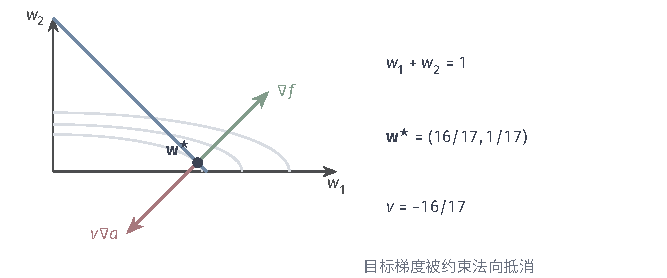
\includegraphics[width=112mm]{figures/00-shared/mathematical-preliminaries-upper/00-shared/tikz/mathematical-language-combinatorics-analysis-optimization-comprehension-additions/kkt-normal-balance.pdf}
  \caption{最小化$(w_1^2+16w_2^2)/2$约束$w_1+w_2=1$。蓝线为可行直线，灰线等值线，在$(16/17,1/17)$处$\nabla f=(16/17,16/17)$，$\nu\nabla a=(-16/17,-16/17)$，等长反向；箭头长度对应法向贡献。}
  \label{fig:vol1-add-kkt-normal-balance}
\end{figure}

\paragraph{LICQ下的必要性。}
设$f,a_j,g_k$在点附近$C^1$且全部等式与活跃不等式梯度线性无关。把这些梯度行扩充为$\mathbb R^d$的一组基，辅以线性坐标$\bm z$构造映射$\bm T(\bm w)=(\bm a(\bm w),\bm g_I(\bm w),\bm z(\bm w))$，由隐函数定理得局部可逆坐标变换；新坐标中可行域恰为$\bm a=0,\bm g_I\leq0$、$\bm z$自由。局部最优令自由坐标偏导为零、活跃不等式坐标偏导非正，链式法则回到原坐标即逐项给出驻点性、非负性与互补松弛。$f(x)=x$、$x^2\leq0$的驻点式$1=0$无解，说明无资格条件时乘子可能不存在。

\subsection{什么证书足以认证全局最优}

若$f$与$g_k$可微凸、$a_j$仿射，且已找到满足全部KKT的候选，对任意可行点应用一阶凸下界并用驻点、等式变化为零、不等式一阶下界与非负乘子，余项非负，即得全局最优。该充分性不需要LICQ或Slater——资格条件解决的是乘子存在性，候选已带乘子时只看凸结构；非凸例$f(x)=-x^2$在零点满足驻点却是极大点。预算例（例~\ref{ex:opt-kkt-budget}）逐区给出KKT解与零乘子切换点，说明活跃不等于正价格；任何情况下，式~\eqref{eq:opt-duality-certificate}的合法上下界不依赖强对偶就能控制目标差。

\begin{example}[活跃约束与预算例]
\label{ex:opt-scalar-active-constraint}
对$\min(x-2)^2/2$、$x\leq a$，$x^\star=\min\{2,a\}$，乘子$u^\star=(2-a)_+$。
\end{example}

\begin{example}[非负预算分配]
\label{ex:opt-kkt-budget}
求最接近$\bm c=(2,1)^\top$的非负分配：
\[
 \min_{\bm w}\frac12\|\bm w-(2,1)^\top\|_2^2
 \quad\text{s.t.}\quad w_1+w_2\leq\tau,\ -w_1\leq0,\ -w_2\leq0.
\]
$\tau>3$时解$(2,1)^\top$，预算不活跃；$\tau=3$时约束活跃但乘子为零；$1<\tau<3$时解$((\tau+1)/2,(\tau-1)/2)^\top$，预算乘子$(3-\tau)/2$；$0<\tau<1$时解$(\tau,0)^\top$，预算乘子$2-\tau$、第二非负约束乘子$1-\tau$。
\end{example}

\subsection{零间隙与最优证书何时达到}
\label{sec:opt-duality}
\label{sec:opt-affine-certificates}

式~\eqref{eq:opt-duality-certificate}只使用弱对偶：任何合法下界都能与可行上界形成证书，却没有说明最高下界等于原最优值。要判断间隙何时为零，需要先回答三个不同的问题：集外一点能否由线性不等式分离，闭凸函数能否由全部仿射下界重建，线性约束不可行时能否给出有限维证书。下面依次建立这些工具，再说明线性规划与一般凸约束分别需要什么条件。

\subsubsection{仿射分离与凸共轭}

投影的法向不等式不仅描述最近点，还能把“点不属于闭凸集”变成一个可核验的线性证书。

\begin{theorem}[闭凸集外一点的严格分离]
\label{thm:opt-projection-separation}
设$C\subseteq\mathbb{R}^d$非空、闭且凸，$\bm z\notin C$。则存在
$\bm a\neq\bm0$和$c\in\mathbb R$，使
\[
 \langle\bm a,\bm x\rangle\leq c
 <\langle\bm a,\bm z\rangle
 \quad\text{对所有 }\bm x\in C.
\]
\end{theorem}

\begin{proof}
由投影小节的证明，$\bm p=\Pi_C(\bm z)$存在且唯一，并满足
$\langle\bm z-\bm p,\bm x-\bm p\rangle\leq0$对所有$\bm x\in C$成立。
取$\bm a=\bm z-\bm p$和$c=\langle\bm a,\bm p\rangle$。由于$\bm z\notin C$，
$\bm a\neq\bm0$，并且
$\langle\bm a,\bm x\rangle\leq c$，而
$\langle\bm a,\bm z\rangle=c+\lVert\bm a\rVert_2^2>c$。
\end{proof}

\begin{definition}[支撑超平面与凸锥]
\label{def:opt-supporting-hyperplane-cone}
设$C\subseteq\mathbb R^d$非空，$\bm a\neq\bm0$。若$C$全部位于
$\{\bm x:\langle\bm a,\bm x\rangle\leq c\}$，并且至少有一点取等号，
则等号超平面称为$C$的支撑超平面（supporting hyperplane）。
非空集合$K$若对所有$\bm u,\bm v\in K$、$\alpha,\beta\geq0$都有
$\alpha\bm u+\beta\bm v\in K$，称为凸锥（convex cone）。
\end{definition}

若$\bm p$位于闭凸集$C$的边界，可取集外点列$\bm z^{(k)}\to\bm p$，对每个点应用严格分离并把法向量归一化。单位球的紧性给出收敛子列，极限法向量$\bm a\neq\bm0$满足
$\langle\bm a,\bm x\rangle\leq\langle\bm a,\bm p\rangle$对所有$\bm x\in C$成立。因此边界处至少有一个支撑方向，但在棱角处法向量未必唯一。分离定理需要集合闭；对偶中由扰动产生的凸集未必闭，所以这一步本身还不是一般强对偶定理。

分离用仿射函数区分点与集合。对目标函数，可以固定斜率，寻找该斜率下最高的全域仿射下界，再问所有斜率是否足以恢复原函数。上图集
$\operatorname{epi}f=\{(\bm x,r):r\geq f(\bm x)\}$凸当且仅当$f$凸，闭当且仅当$f$下半连续。

\begin{definition}[凸共轭与双共轭]
\label{def:opt-conjugate}
给定适当函数$f:\mathbb R^d\to\mathbb R\cup\{+\infty\}$，其\term{凸共轭}（convex conjugate）定义为
\begin{equation}
 f^*(\bm y)=\sup_{\bm x\in\mathbb R^d}
 \{\langle\bm y,\bm x\rangle-f(\bm x)\},
 \qquad
 f^{**}(\bm x)=\sup_{\bm y\in\mathbb R^d}
 \{\langle\bm y,\bm x\rangle-f^*(\bm y)\}.
 \label{eq:opt-conjugate-biconjugate}
\end{equation}
两个上确界都在整个$\mathbb R^d$上取。$f^*$允许取$+\infty$；若$f^*\equiv+\infty$，则$f^{**}\equiv-\infty$。除此之外，$f^{**}$不取$-\infty$，但仍可能取$+\infty$。
\end{definition}

$f(\bm x)=+\infty$的点不贡献有限共轭候选。固定斜率$\bm y$时，$f^*(\bm y)$是让
$\langle\bm y,\bm x\rangle-f^*(\bm y)$在全域不超过$f$所需的最小截距修正。

\begin{example}[由斜率重建二次函数]
\label{ex:opt-quadratic-conjugate-envelope}
仍取图~\ref{fig:opt-convex-chord-tangent}中的$f(x)=x^2/2$。固定直线斜率$y$，配方得到
\[
 yx-\frac{x^2}{2}=\frac{y^2}{2}-\frac{(x-y)^2}{2}.
\]
右边在$x=y$时达到最大值，所以$f^*(y)=y^2/2$。该共轭值确定了这个斜率下最高的仿射下界
\begin{equation}
 \ell_y(x)=yx-\frac{y^2}{2},\qquad
 f(x)-\ell_y(x)=\frac{(x-y)^2}{2}\geq0.
 \label{eq:opt-quadratic-affine-minorant}
\end{equation}
直线$\ell_y$在$x=y$处与抛物线相切；再提高截距，就会在该点超过$f$。固定输入$x$并让斜率变化，每条直线都在$f$下方，而$y=x$在该输入处取等，因此
\[
 f^{**}(x)=\sup_{y\in\mathbb R}\ell_y(x)=\frac{x^2}{2}.
\]
图~\ref{fig:opt-conjugate-affine-envelope}只画三个斜率。它们的逐点最大值仍是折线；纳入全部实数斜率后，才在每个输入处恢复抛物线。
\end{example}

\begin{figure}[htbp]
 \centering
 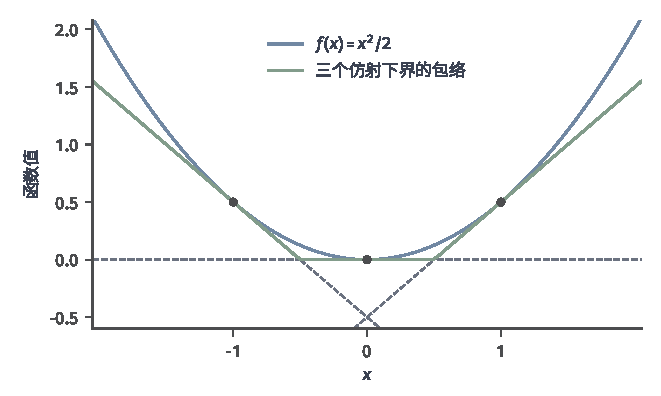
\includegraphics[width=112.0mm]{figures/00-shared/mathematical-preliminaries-upper/04-optimization/matplotlib/opt-conjugate-affine-envelope/figure.pdf}
 \caption{$f(x)=x^2/2$与斜率$y=-1,0,1$对应的仿射下界$\ell_y(x)=yx-y^2/2$。蓝实线为抛物线，三条灰虚线为下界，绿实线为这三条下界的逐点最大值。三个实心点标出相切位置；有限个斜率留下的间隙，在取全部斜率的上确界时消失。图为解析教学示例。}
 \label{fig:opt-conjugate-affine-envelope}
\end{figure}

没有任何仿射下界时，共轭对每个斜率都为无穷。例如$f(x)=-x^2$满足
$f^*(y)=\sup_x\{yx+x^2\}=+\infty$，双共轭因而恒为$-\infty$；适当性本身不能排除这种情形。由定义立即有Fenchel--Young不等式
\[
 f(\bm x)+f^*(\bm y)\geq\langle\bm y,\bm x\rangle,
\]
以及$f^{**}\leq f$。双共轭是连续仿射函数族的上确界，因而凸且下半连续；它不要求每个上确界都由有限斜率达到。

\begin{theorem}[有限维Fenchel--Moreau定理]
\label{thm:opt-fenchel-moreau}
设$f:\mathbb R^d\to\mathbb R\cup\{+\infty\}$适当、下半连续且凸。则$f^{**}=f$在全部$\mathbb R^d$上成立，包括$f(\bm x)=+\infty$的点。因此$f$恰好是全部连续仿射下界的逐点上确界。
\end{theorem}

\begin{proof}
上图集$\operatorname{epi}f$非空、闭且凸。任取$\bm x_0\in\operatorname{dom}f$及$t_0<f(\bm x_0)$，对上图与外点$(\bm x_0,t_0)$使用定理~\ref{thm:opt-projection-separation}。必要时改变分离法向量的符号，可写成
\[
 \langle\bm a,\bm x_0\rangle+b t_0<c
 \leq\langle\bm a,\bm z\rangle+b r
 \quad\text{对所有 }(\bm z,r)\in\operatorname{epi}f.
\]
上图沿$r$向上无界，故$b\geq0$；若$b=0$，取$(\bm z,r)=(\bm x_0,f(\bm x_0))$便矛盾，所以$b>0$。重排得到一个全域仿射下界
$\ell_0(\bm z)=\langle\bm p_0,\bm z\rangle-\beta_0\leq f(\bm z)$，也就保证$f^*(\bm p_0)$有限。

现任取$\bm x$和实数$t<f(\bm x)$，再次严格分离$(\bm x,t)$与上图。若所得竖直系数$b>0$，立即得到仿射下界$\ell$，满足$\ell(\bm x)>t$。若$b=0$，分离不等式为
$\langle\bm a,\bm x\rangle<c\leq\langle\bm a,\bm z\rangle$。将它与
$\varepsilon(r-\ell_0(\bm z))\geq0$相加，得到
\[
 \langle\bm a-\varepsilon\bm p_0,\bm z\rangle+\varepsilon r
 \geq c-\varepsilon\beta_0.
\]
原分离间隙为正，所以取足够小的$\varepsilon>0$后，$(\bm x,t)$处仍满足严格反向不等式；新的竖直系数为正，因而仍得到$\ell\leq f$且$\ell(\bm x)>t$。

将下界写成$\ell(\bm z)=\langle\bm y,\bm z\rangle-\beta$，有$f^*(\bm y)\leq\beta$，所以
\[
 f^{**}(\bm x)\geq\langle\bm y,\bm x\rangle-f^*(\bm y)
 \geq\ell(\bm x)>t.
\]
若$f(\bm x)$有限，令$t\uparrow f(\bm x)$；若$f(\bm x)=+\infty$，让$t$任意增大。两种情形都给出$f^{**}(\bm x)\geq f(\bm x)$，结合反向不等式即得结论。
\end{proof}

闭性不能省略。若$f=\iota_{(0,1)}$，则$f^*(y)=\max\{0,y\}$，但双共轭为$\iota_{[0,1]}$，在两个端点补上零值；仿射下界不能区分边界点与从内部趋近的极限。即使$f=f^{**}$，边界处也未必有有限最优斜率：对$x\geq0$时$f(x)=-\sqrt{x}$、负半轴取$+\infty$，在$x=0$不存在有限次梯度，但一列仿射下界仍可把函数值逼近到零。因此值重建与共轭上确界达到是两个问题。

共轭还能直接计算对偶下界。对
$\min_{\bm w}\{f(\bm w):\bm a^\top\bm w=b\}$，固定乘子$\nu$有
\[
 q(\nu)=\inf_{\bm w}\{f(\bm w)+\nu(\bm a^\top\bm w-b)\}
 =-f^*(-\nu\bm a)-\nu b.
\]
若$f(\bm w)=\lVert\bm w\rVert_2^2/2$且$\bm a\neq\bm0$，则
$f^*(\bm y)=\lVert\bm y\rVert_2^2/2$，$q$在
$\nu^\star=-b/\lVert\bm a\rVert_2^2$达到
$b^2/(2\lVert\bm a\rVert_2^2)$；原始点
$\bm w^\star=b\bm a/\lVert\bm a\rVert_2^2$也取同值。共轭在这里计算下界，Fenchel--Moreau说明闭凸函数不会在收集全部仿射下界时损失函数值；具体约束问题是否零间隙仍须另外证明。

\subsubsection{线性规划强对偶}

线性约束的下一步是把不可行性写成另一组线性不等式。线性规划强对偶将由这种证书推出，不以双共轭等式替代证明。先建立有限生成锥与多面体像的闭性\scite{math-boyd2004convex}

\begin{lemma}[有限生成锥的闭性]
\label{lem:opt-finitely-generated-cone}
给定$\bm a_1,\ldots,\bm a_r\in\mathbb R^m$，集合
\[
 K=\left\{\sum_{i=1}^r\alpha_i\bm a_i:\alpha_i\geq0\right\}
\]
是闭凸锥。
\end{lemma}

\begin{proof}
凸性和锥性质由非负线性组合直接得到。先说明每个$\bm x\in K$都能由一组线性无关的生成向量作非负组合。若某个表示使用的生成向量线性相关，就存在非零系数$\bm\gamma$使
$\sum_i\gamma_i\bm a_i=\bm0$；必要时改变符号，使至少一个$\gamma_i>0$。从原系数中减去$t\bm\gamma$，其中
$t=\min_{\gamma_i>0}\alpha_i/\gamma_i$，仍保持全部系数非负，并使至少一个系数变为零。重复后得到线性无关的表示。

现取$\bm x^{(k)}\in K$且$\bm x^{(k)}\to\bm x$。线性无关的生成子集只有有限多个，故可取子列，使每个$\bm x^{(k)}$都使用同一个子集$J$。以这些向量为列组成满列秩矩阵$\bm A_J$，相应非负系数满足
\[
 \bm\alpha^{(k)}=(\bm A_J^\top\bm A_J)^{-1}\bm A_J^\top\bm x^{(k)}
 \longrightarrow
 (\bm A_J^\top\bm A_J)^{-1}\bm A_J^\top\bm x.
\]
极限系数仍逐项非负，且$\bm x$等于$\bm A_J$乘该极限系数，故$\bm x\in K$。
\end{proof}

\begin{lemma}[有限维多面体的线性像]
\label{lem:opt-polyhedral-image}
有限维多面体在线性映射下的像仍是多面体，因而是闭集。
\end{lemma}

\begin{proof}
设$P=\{\bm u:\bm B\bm u\leq\bm d\}$，线性映射为$\bm v=\bm T\bm u$。其图像
\[
 \{(\bm u,\bm v):\bm B\bm u\leq\bm d,\ \bm v=\bm T\bm u\}
\]
是多面体，而$\bm T P$是该图像消去$\bm u$后的坐标投影。对一个待消变量，Fourier--Motzkin消元分别收集其系数为正、为负和为零的不等式；每一对正、负系数不等式消去该变量，零系数不等式原样保留。逐个消去$\bm u$的坐标，就得到$\bm T P$的有限非严格线性不等式表示。它是有限个闭半空间的交，因而闭。
\end{proof}

\begin{theorem}[Farkas择一定理]
\label{thm:opt-farkas}
给定$\bm M\in\mathbb R^{m\times d}$和$\bm r\in\mathbb R^m$，下列两个系统恰有一个可行：
\[
 \bm M\bm x=\bm r,\quad\bm x\geq\bm0;
 \qquad
 \bm M^\top\bm z\geq\bm0,\quad\bm r^\top\bm z<0.
\]
\end{theorem}

\begin{proof}
两者不能同时成立，因为若都成立，则
$0>\bm r^\top\bm z=\bm x^\top\bm M^\top\bm z\geq0$，矛盾。
若第一个系统不可行，$\bm r$不属于锥
$K=\{\bm M\bm x:\bm x\geq\bm0\}$。它由$\bm M$的有限个列向量生成，故由引理~\ref{lem:opt-finitely-generated-cone}可知$K$是闭凸锥。对$K$与$\bm r$应用定理~\ref{thm:opt-projection-separation}，得到$\bm a$和$c$，使
$\langle\bm a,\bm k\rangle\leq c<\langle\bm a,\bm r\rangle$。由于$\bm0\in K$，有$c\geq0$；又因为$t\bm k\in K$对所有$t\geq0$成立，必有
$\langle\bm a,\bm k\rangle\leq0$，否则充分大的$t$会超过$c$。令$\bm z=-\bm a$，可得
$\langle\bm z,\bm r\rangle<0$且
$\langle\bm z,\bm k\rangle\geq0$对所有$\bm k\in K$成立，特别地
$\bm M^\top\bm z\geq\bm0$。第二个系统可行。
\end{proof}

\begin{theorem}[有限维线性规划强对偶]
\label{thm:opt-lp-strong-duality}
考虑标准型原问题与对偶问题
\[
 \min_{\bm x\geq\bm0}\bm c^\top\bm x
 \quad\text{s.t.}\quad\bm A\bm x=\bm b,
 \qquad
 \max_{\bm y}\bm b^\top\bm y
 \quad\text{s.t.}\quad\bm A^\top\bm y\leq\bm c.
\]
若原问题可行且有限下确界为$p^\star$，则原问题与对偶问题都有最优解，且两个最优值都等于$p^\star$。
\end{theorem}

\begin{proof}
原始可行域$P=\{\bm x:\bm A\bm x=\bm b,\ \bm x\geq\bm0\}$是非空多面体。由引理~\ref{lem:opt-polyhedral-image}，其目标值集合
\[
 W=\{\bm c^\top\bm x:\bm x\in P\}
\]
是$\mathbb R$中的非空多面体。集合$W$下有界，一维多面体又包含自己的有限下端点，故$p^\star=\inf W$属于$W$，原始最优解达到。

对任意$\varepsilon>0$，系统
\[
 \bm A\bm x=\bm b,\quad
 \bm c^\top\bm x+s=p^\star-\varepsilon,\quad
 \bm x\geq\bm0,\ s\geq0
\]
不可行，否则会有目标值小于$p^\star$的原始可行点。对增广系统应用定理~\ref{thm:opt-farkas}，存在$(\bm y_\varepsilon,\gamma_\varepsilon)$满足
\[
 \bm A^\top\bm y_\varepsilon+\gamma_\varepsilon\bm c\geq\bm0,
 \quad\gamma_\varepsilon\geq0,
 \quad\bm b^\top\bm y_\varepsilon
 +\gamma_\varepsilon(p^\star-\varepsilon)<0.
\]
取任一原始可行$\bar{\bm x}$并与第一式作内积，可知$\gamma_\varepsilon>0$；若它为零，就会与最后一式矛盾。令
$\widehat{\bm y}_\varepsilon=-\bm y_\varepsilon/\gamma_\varepsilon$，便有
$\bm A^\top\widehat{\bm y}_\varepsilon\leq\bm c$且
$\bm b^\top\widehat{\bm y}_\varepsilon>p^\star-\varepsilon$。

记对偶可行多面体为$D=\{\bm y:\bm A^\top\bm y\leq\bm c\}$，目标值集合为
$V=\{\bm b^\top\bm y:\bm y\in D\}$。上面的构造说明$D$非空，而且$\sup V\geq p^\star$；弱对偶给反向不等式，所以$\sup V=p^\star$。由引理~\ref{lem:opt-polyhedral-image}，$V$是一维多面体；它有有限上确界，因而包含上端点$p^\star$。对偶最优解也达到，并与原问题同值。
\end{proof}

\begin{example}[二维资源分配的原始与对偶证书]
\label{ex:opt-resource-lp-duality}
考虑
\[
 \max_{x_1,x_2\geq0}3x_1+2x_2
 \quad\text{s.t.}\quad
 2x_1+x_2\leq4,\quad x_1+2x_2\leq4.
\]
为两类资源设置价格$u_1,u_2\geq0$。要使Lagrangian关于$\bm x\geq\bm0$的上确界有限，必须有
$2u_1+u_2\geq3$和$u_1+2u_2\geq2$；此时上界为$4u_1+4u_2$。原始点
$(x_1,x_2)=(4/3,4/3)$可行，值为$20/3$；对偶点
$(u_1,u_2)=(4/3,1/3)$可行，也取$20/3$。弱对偶因此认证二者同时最优，互补松弛亦逐项成立。
\end{example}

不可行、无界与未达到必须分开。Farkas向量证明约束不可行；若原问题沿可行射线无限改善，弱对偶只说明没有乘子给出有限下界，在线性规划标准型中表现为对偶不可行，不能据此断言乘子候选集合本身为空。若只有下确界而没有达到，则仍不能展示原始最优点。

\subsubsection{Slater资格}

一般凸问题的有效定义域可能落在低维仿射空间中。若仍要求环境空间中的普通内部非空，就会把线段、平面等合法定义域排除在外；相对内部只在定义域自身张成的仿射空间内寻找余量。

\begin{definition}[仿射包与相对内部]
\label{def:opt-affine-hull-relative-interior}
对非空集合$C\subseteq\mathbb R^d$，其\term{仿射包}（affine hull）是全部有限仿射组合
$\sum_i\alpha_i\bm x_i$组成的集合，其中$\bm x_i\in C$、$\sum_i\alpha_i=1$，权重可以为负。点$\bm x\in C$属于\term{相对内部}（relative interior），是指存在$r>0$使
$B(\bm x,r)\cap\operatorname{aff}C\subseteq C$。
\end{definition}

平面中的线段没有二维内部，但去掉两个端点后就是它的相对内部。这个概念使严格可行性只要求在共同有效定义域的真实维度内留出余量。

\begin{theorem}[Slater条件下的强对偶]
\label{thm:opt-slater-strong-duality}
设$f$和不等式函数$g_k$都是适当凸函数，并具有共同凸有效定义域$D$；等式约束为仿射约束$\bm A\bm w=\bm b$。若存在
\[
 \bar{\bm w}\in\operatorname{ri}D,\qquad
 \bm A\bar{\bm w}=\bm b,\qquad
 g_k(\bar{\bm w})<0\quad\text{对所有 }k,
\]
并且原问题最优值有限，则原、对偶最优值相等，且存在最优对偶乘子。
\end{theorem}

共同定义域$D$是这些函数同时取有限值的区域。相对内部处理低维定义域，严格不等式提供可行余量；仿射等式不要求严格化。该定理的一般证明需要更一般的凸集分离，并处理约束值与目标值组成的扰动集合边界；这类集合未必闭，不能直接套用定理~\ref{thm:opt-projection-separation}。本章不把这一部分压缩成伪证明，后续使用时逐项核对共同定义域、仿射等式、严格可行点与有限最优值。

Slater条件不保证原始最小点达到：$\min_x e^x$没有不等式约束，最优值为$0$却没有原始最优点。反过来，凸问题一旦已经找到KKT候选，其全局充分性不需要Slater；Slater负责保证零间隙与最优乘子的存在，不替代原始达到性。预算例在$\tau>0$时有严格可行点，闭域上的强制目标另行保证原始达到，因此它同时具备可行、原始达到、零间隙与对偶达到。这四项结论必须分别核验。

\section{收敛速度与计算预算的比较}

凸光滑原始目标与非空闭凸可行域上，投影梯度给$O(1/T)$原始目标差；对偶光滑且乘子达到时$d^\star-q$同为$O(1/T)$，非光滑残差按次梯度累计界评价；即使零间隙，实际全局证书仍用独立恢复的$U-q$。二次罚的参数极限结论不是按外层次数的速率，精确罚还要看内层方法的实际精度。停止时先报告实际违反量，再报告合法下界与可行上界之差；预算例残差按$2^{-t}$、间隙按$4^{-t}$缩小，依赖特定二次结构与步长。总预算要合计外层迭代、梯度／残差求值、投影或内层求解成本，不能只比外层次数。

\section{误差传播与约束参数敏感性}

\subsection{计算误差怎样影响轨迹与停止}

投影轨迹误差按13.2.5传播；近似对偶内层的累计项与可信下界按13.4.3进入；罚方法比较式控制的是违反量。数值残差应分项报告：即使无约束凸目标，梯度$\delta$在$f(x)=\epsilon x^2/2$下对应目标差$\delta^2/(2\epsilon)$，小KKT残差脱离尺度不构成目标差证书，全局差距仍由式~\eqref{eq:opt-duality-certificate}承担。

\subsection{约束参数怎样改变最优解}

\paragraph{内点分支。}
对依赖$\theta$的无约束目标，驻点方程$\varphi_z(z,\theta)=0$在$\varphi_{zz}\neq0$时由隐函数定理给出局部分支；例$\varphi(z,\theta)=\frac12(1+\theta)z^2-\theta z$（$\theta>-1$）的解$z^\star=\theta/(1+\theta)$，导数$1/(1+\theta)^2$可由隐式与显式两种方式复算，但分支是否全局最优仍要另行核验。

\paragraph{固定活跃集的KKT系统。}
固定活跃集$I$，把驻点、等式与活跃不等式等号条件写成$\bm\Phi(\bm w,\bm\nu,\bm\alpha_I,\tau)=\bm0$。Jacobian可逆时局部解连续可微；所需的是完整KKT块矩阵
\[
 \begin{bmatrix}
 \nabla_{\bm w,\bm w}^2\mathcal L&\bm A_I^\top\\
 \bm A_I&\bm0
 \end{bmatrix}
\]
可逆，原目标Hessian可逆并不足够。若$\bm A_I$满行秩且Lagrangian Hessian在$\ker\bm A_I$上正定，齐次方程先逼方向进核、再内积逼其为零，块矩阵可逆；活跃乘子严格为正与未活跃严格余量使小邻域保持同一活跃集。预算例$1<\tau<3$时解导数$(1/2,1/2)^\top$、$0<\tau<1$时$(1,0)^\top$，$\tau=1$解连续但导数改变。

\subsection{约束参数怎样改变最优值}

内点驻点使链式法则中含解导数的项消失：$V'(\theta)=\partial\varphi/\partial\theta|_{z=z^\star}$，这是\term{包络定理}的基本机制，但解导数本身仍存在。约束写成$g_k(\bm w)-\tau_k\leq0$时，对保持全局最优的分支，
\[
 \frac{\partial V}{\partial\tau_k}=-\alpha_k^\star
\]
（未活跃乘子取零）；只有该分支继续全局最优（凸问题中KKT充分性保证这一点），局部分支值才等于全局最优值。预算例值函数
\[
 V(\tau)=
 \begin{cases}
 0,&\tau\geq3,\\
 (3-\tau)^2/4,&1\leq\tau\leq3,\\
 ((2-\tau)^2+1)/2,&0<\tau\leq1
 \end{cases}
\]
逐区间满足$V'(\tau)=-\alpha_{\rm bud}^\star$；放宽预算$\Delta\tau$的一阶收益是$\alpha^\star\Delta\tau$，这是值变化率而非参数移动量。

图~\ref{fig:opt-budget-active-set}沿同一预算轴展示解坐标与乘子。
\begin{figure*}[htbp]
  \centering
  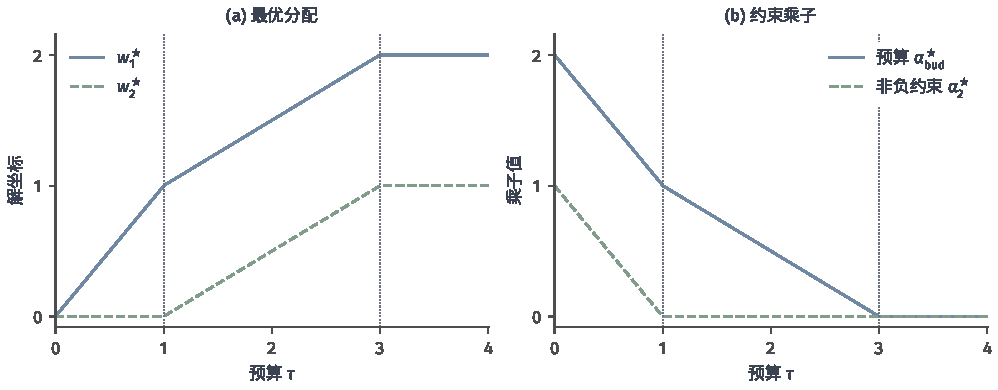
\includegraphics[width=169.0mm]{figures/00-shared/mathematical-preliminaries-upper/04-optimization/matplotlib/opt-budget-active-set/figure.pdf}
  \caption{例~\ref{ex:opt-kkt-budget}的解析解。左图为两个最优分配坐标，右图为预算乘子与第二非负约束乘子。竖线标出$\tau=1,3$；切换点约束可取等号而乘子为零。}
 \label{fig:opt-budget-active-set}
\end{figure*}

\section{本章小结}

三条约束路线各改一个计算对象：投影保持落点可行，惩罚通过违反量改变比较目标，乘子与对偶建立梯度平衡和下界。它们可以组合，但每次组合都要重新写清内层域、被对偶化的约束与实际目标。证书分三层：LICQ支持局部KKT必要性，凸结构支持KKT候选的全局充分性，合法下界配合可行上界直接控制目标差；Farkas认证线性不可行，LP强对偶与Slater分别给出不同结构上的零间隙依据，任何一项都不能替代全部达到性核验。残差驱动的对偶更新改善下界，内层点仍需恢复原始可行，近似内层误差必须进入累计界与可信下界；最优值对约束参数的变化率由活跃乘子给出，且依赖活跃集、完整KKT系统与分支全局最优。

\chapter{计算预算有限时的近似优化}
\label{chap:approximate-optimization}

更新公式可以写成一条，执行它却要读取数据、求解子问题并重复多轮。当这些成本超过预算，就必须说明在哪一环让步、引入的误差如何受控。本章固定原问题与预算口径，按被改变的计算对象组织：14.1放宽候选可行集并恢复原解，14.2用主化代理替换当步目标，14.3限制每轮更新的变量范围，14.4改变方向的读取、聚合与反向规则。四种简化不互斥，可以组合；但每种简化只直接控制被简化后的问题，返回候选仍须按原问题的可行性与误差标准核验。

\section{松弛域的构造与原解恢复}

\subsection{精确凸包的基准与恢复问题}

离散选择中变量只能取$0$或$1$，孤立点上没有斜率，无法沿梯度移动；一种做法是把候选放进包含它们的连续凸集，这类放宽称为\term{凸松弛}，可先求较易问题的界，再恢复原解。对非空有限集$S=\{\bm s_1,\ldots,\bm s_N\}$，其凸包
\[
 \operatorname{conv}(S)
 =\left\{\sum_{i=1}^N\alpha_i\bm s_i:
 \alpha_i\geq0,\ \sum_i\alpha_i=1\right\}
\]
是包含$S$的最小凸集；凸包的基本性质已在凸性讨论中建立。若原目标只在$S$上定义，还须选定在$S$上与之一致的连续延拓，才能谈松弛问题的目标。

\paragraph{线性值保持。}
对线性目标$\bm c^\top\bm x$，任意凸包点的目标值是原候选值的加权平均，故$\min_{\operatorname{conv}(S)}\bm c^\top\bm x=\min_S\bm c^\top\bm x$，最大化同理；有限集保证极值达到。但数值相等没有规定求解器返回哪个点。凸集的极点是不能写成非平凡平均的点；线性目标的最优面$K^\star=\{\bm x\in K:\bm c^\top\bm x=M\}$在$K=\operatorname{conv}(S)$时正是原最优点的凸包——给次优点正权重会严格拉低平均值。当$S\subseteq\mathbb Z^d$时最优面含整数极点（可在有限个整数最优点中逐坐标取字典序最大者），但这并不保证任意连续输出都是整数点。

三点集$S=\{(0,0),(1,0),(0,1)\}$同时说明两件事：原候选$(1,0)$与分数点$(1/2,1/2)$在线性目标$x_1+x_2$下值都为$1$，最优数值确实能由原候选取得；但$(1/2,1/2)$本身不属于$S$，求解器返回它仍需恢复规则。

\subsection{线性约束的外逼近松弛}

精确凸包的完整不等式描述可能难以获得，只保留局部约束通常得到更大、更易求解的多面体；对最小化它给更松的下界。容量例
\[
 \max_{x_1,x_2\in\{0,1\}}x_1+x_2
 \quad\text{s.t.}\quad 2x_1+2x_2\leq3
\]
的整数最优值为$1$；放宽到$[0,1]^2$后$(3/4,3/4)$可行且值为$3/2$。四舍五入得$(1,1)$违反容量（容量为$4$），向下取整得$(0,0)$虽可行却损失全部收益。松弛值与原最优值之差$3/2-1=1/2$称为\term{整数间隙}（integrality gap）；松弛值、恢复规则可行性与恢复后损失必须分别分析。

图~\ref{fig:opt-hull-relaxation}并列精确凸包与局部松弛。
\begin{figure*}[htbp]
  \centering
  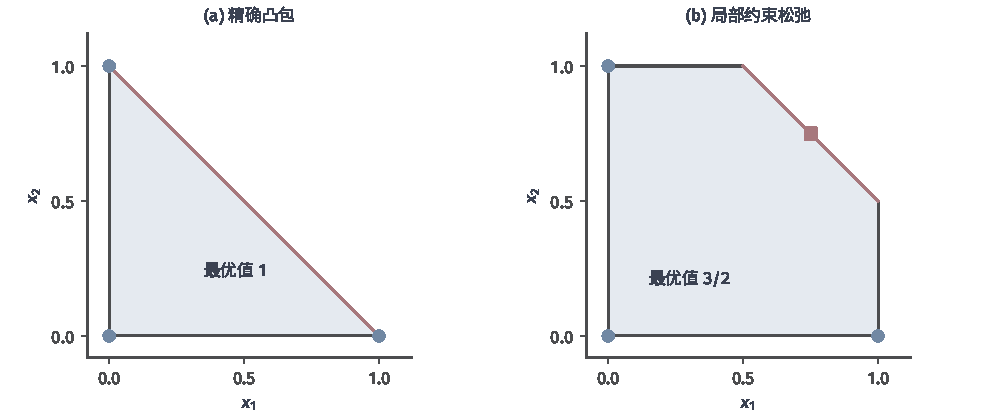
\includegraphics[width=169.0mm]{figures/00-shared/mathematical-preliminaries-upper/04-optimization/matplotlib/opt-hull-relaxation/figure.pdf}
  \caption{最大化$x_1+x_2$的两种放宽。左图精确凸包满足$x_1+x_2\leq1$；右图局部松弛满足$0\leq x_i\leq1$与$x_1+x_2\leq3/2$。实心圆为整数可行点，方形为分数最优点$(3/4,3/4)$，粗边标出最优面。}
 \label{fig:opt-hull-relaxation}
\end{figure*}

\subsection{半正定松弛法}

含乘积$x_ix_j$时引入对称矩阵$\bm X$，精确表示要求$\bm X=\bm x\bm x^\top$（非凸等式），放宽为
\[
 \begin{bmatrix}1&\bm x^\top\\\bm x&\bm X\end{bmatrix}\succeq\bm0
 \quad\Longleftrightarrow\quad \bm X-\bm x\bm x^\top\succeq\bm0,
\]
等价性由$(t+\bm x^\top\bm v)^2+\bm v^\top(\bm X-\bm x\bm x^\top)\bm v$配方核对。真实乘积满足新约束，新约束却允许偏离真实乘积；新增矩阵有$O(d^2)$个元素，需求解锥约束。返回$(\widehat{\bm x},\widehat{\bm X})$后要分别核验原约束与$\widehat{\bm X}=\widehat{\bm x}\widehat{\bm x}^\top$，矩阵提升本身不完成原解恢复。集合函数的连续扩展还须针对所选扩展检验凸凹性，“次模”（离散次模不等式）本身不判定延拓的凸性；二值成对能量的图割表示是后续图章在特定条件下展开的接口。

\section{主化—最小化代理法（MM）}

\subsection{MM的代理构造、接受与误差}

梯度下降的闭式步长来自下降引理给出的可计算二次上界。把这一思想一般化：在当前点构造一个处处不低于原目标、又在当前点贴合的简单函数。

\begin{definition}[主化代理与MM更新]
\label{def:opt-majorization-minimization}
给定目标$F:C\to\mathbb R$与当前点$\bm w^{(t)}\in C$，代理$Q(\bm w\mid\bm w^{(t)})$满足
\[
 F(\bm w)\leq Q(\bm w\mid\bm w^{(t)}),\qquad
 F(\bm w^{(t)})=Q(\bm w^{(t)}\mid\bm w^{(t)})\quad(\forall\bm w\in C).
\]
若新点满足代理值不增$Q(\bm w^{(t+1)}\mid\bm w^{(t)})\leq Q(\bm w^{(t)}\mid\bm w^{(t)})$，称为\term{主化--最小化方法}（majorization--minimization，MM）的改善更新。
\end{definition}

改善链为
\[
 F(\bm w^{(t+1)})
 \leq Q(\bm w^{(t+1)}\mid\bm w^{(t)})
 \leq Q(\bm w^{(t)}\mid\bm w^{(t)})
 =F(\bm w^{(t)}),
\]
三步分别用全局上界、代理改善与切触；上界只在局部有效时，新点越界就断链。$L$光滑目标的下降引理二次型就是代理：全空间精确最小化给$1/L$梯度步，闭凸集上给投影梯度。不精确最小化时，记代理最优值$Q^{\star,(t)}$与改善空间$\Delta^{(t)}=Q(\bm w^{(t)}\mid\cdot)-Q^{\star,(t)}$，若
\[
 Q(\bm w^{(t+1)}\mid\bm w^{(t)})\leq Q^{\star,(t)}+\epsilon^{(t)},
\]
则$F(\bm w^{(t+1)})\leq F(\bm w^{(t)})-\Delta^{(t)}+\epsilon^{(t)}$；只有$\epsilon^{(t)}\leq\Delta^{(t)}$才保证本轮不增。原目标有有限下界时$\sum_{t<T}\Delta^{(t)}\leq F(\bm w^{(0)})-\inf_CF+\sum_t\epsilon^{(t)}$。数值例$F(x)=x^2/2$、$Q(x\mid1)=(x-1/2)^2+1/4$中，求到$x=3/4$仍改善（$9/32<1/2$），返回$x=5/4$时代理误差$9/16$超过改善量$1/4$，原目标反升为$25/32$。

图~\ref{fig:opt-majorizer-versus-tangent}对照代理上界与同斜率切线。
\begin{figure}[htbp]
  \centering
  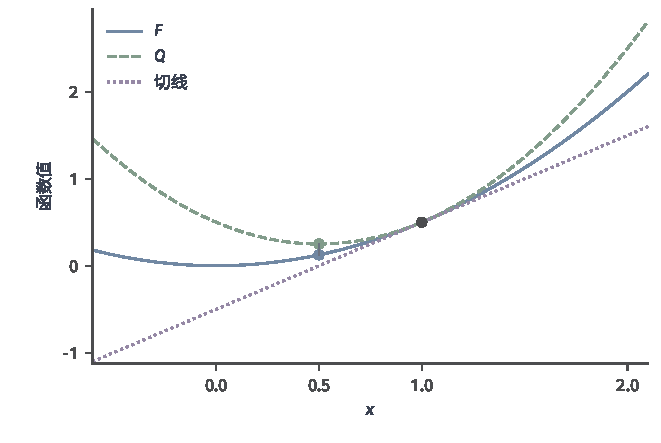
\includegraphics[width=112.0mm]{figures/00-shared/mathematical-preliminaries-upper/04-optimization/matplotlib/opt-majorizer-versus-tangent/figure.pdf}
  \caption{代理上界与切线的区别。蓝线$F(x)=x^2/2$，绿虚线为当前点$1$处的主化代理，紫点线为同点切线$x-1/2$。三者在当前点同值同斜率，但切线位于目标下方，不能使用MM的上界链。}
 \label{fig:opt-majorizer-versus-tangent}
\end{figure}

\subsection{MM的残差实现：IRLS}

平方代价使残差$10$的贡献是残差$1$的百倍。保持残差定义不变，改用增长较慢的代价$F(\bm w)=\frac12\sum_i\rho(r_i(\bm w)^2)$：平方损失$\rho(s)=s$；尺度$c>0$下Cauchy代价$c^2\log(1+s/c^2)$；Tukey代价在$s\leq c^2$时为$c^2[1-(1-s/c^2)^3]/3$、其后恒为$c^2/3$。单项对残差的斜率分别为$r$、$r/(1+r^2/c^2)$和$r(1-r^2/c^2)^2\mathbb I\{|r|\leq c\}$，大残差处边际代价减弱；参数梯度还乘$\nabla r_i$，且代价非凸，初始化与尺度影响驻点。

若$\rho$可微、非减且关于$s$凹，凹函数在切线下，故$\rho(s)\leq\rho(s_0)+\rho'(s_0)(s-s_0)$。在当前残差$s_i^{(t)}=r_i(\bm w^{(t)})^2$处构造代理
\begin{equation}
 Q(\bm w\mid\bm w^{(t)})
 =\mathrm{const}^{(t)}
 +\frac12\sum_i a_i^{(t)}r_i(\bm w)^2,
 \qquad a_i^{(t)}=\rho'(s_i^{(t)})\geq0,
 \label{eq:opt-irls-majorizer}
\end{equation}
每轮“算权重—固定权重解加权最小二乘—重算残差权重”，即\term{迭代重加权最小二乘}（iteratively reweighted least squares，IRLS）。Cauchy权重为$(1+s_i/c^2)^{-1}$，Tukey权重为$(1-s_i/c^2)^2\mathbb I\{s_i\leq c^2\}$；权重来自同一目标的切线，不能任意重设。线性残差时子问题是加权最小二乘（权重平方根各行相乘后用QR/SVD），非线性残差时可在内部调用Gauss--Newton或LM，但一次线性化方程解不保证完整代理下降，必须核验代理值。用常数$w$拟合$0,0,10$，Cauchy（$c=1$，$w^{(0)}=0$）首轮权重$1,1,1/101$给$w^{(1)}=10/203$；Tukey可能让全部权重为零、代理退化为常数，此时应检查初始化或尺度。永久正则项须原样进入每轮代理，不能与内部控制位移的阻尼混同。

\section{块坐标更新}

本节把一次全变量更新拆成若干小问题，这类按变量块更新的路线称为\term{分块坐标法}。

\subsection{块梯度与块邻近更新}

变量自然分成$\bm u\in\mathbb R^p$、$\bm v\in\mathbb R^q$时，对
\[
 \Phi(\bm u,\bm v)=\frac12\|\bm X\bm u+\bm Z\bm v-\bm y\|_2^2+r(\bm u)+s(\bm v)
\]
可固定其余块，只对当前块作梯度或邻近一步，每完成一块就用同一$\Phi$核验改善。固定$\bm v$时光滑项对$\bm u$的光滑常数为$\|\bm X\|_2^2$，邻近步长取$0<\eta_u\leq1/\|\bm X\|_2^2$；近似输出仍须实际接受条件。

\subsection{块条件最小化：交替最小化}

\term{交替最小化}依次精确或近似求解固定其他块后的条件子问题：
\[
 \Phi(\bm u^{(t+1)},\bm v^{(t)})\leq\Phi(\bm u^{(t)},\bm v^{(t)}),\qquad
 \Phi(\bm u^{(t+1)},\bm v^{(t+1)})\leq\Phi(\bm u^{(t+1)},\bm v^{(t)}),
\]
两条不等式串成同一轮下降，多解时要规定平局选解规则。耦合正定二次例$\Phi(u,v)=\frac12(u-v)^2+\frac12(u-1)^2$给$v^{(t+1)}-1=(v^{(t)}-1)/2$，收敛到$(1,1)$；但$(uv-1)^2$从$(0,0)$出发时，任一块固定为零目标都是常数，平局规则选零就停在目标$1$，而全局最优为$0$——逐块精确、分别凸都不保证全局最优。无约束连续可微时，每块最优给各偏导为零，合起来是联合驻点；联合凸时才足以给全局最优，且还要证明实际迭代到达块最优点。

有限分布变量就是概率单纯形$\bm\Delta_m=\{\bm q:q_i\geq0,\sum_iq_i=1\}$上的向量，块更新后必须留在单纯形内。把$\bm q$投影到$\bm\Delta_2$、目标中心$(0.8,0.4)^\top$的解为$(0.7,0.3)^\top$（共减阈值$0.1$），它真实最小化当前条件目标。EM与变分方法在期望与散度对象建立后复用这里的交替优化与MM核验。副本协调式的对偶分解（改进对偶下界、原目标不逐轮下降）与本节同一原目标上的交替改善是两条路线，不能互相代替。

\section{方向的读取、聚合与变换}

有限和目标
\[
 F_S(\bm w)=\frac1n\sum_{i=1}^n\ell_i(\bm w)+\frac{\lambda}{2}\|\bm w\|_2^2
\]
的完整梯度要读取全部$n$项。以下只用有限概率权重的加权平均（记固定历史后的平均为$\mathbb E^{(t)}$）；长期随机收敛与泛化留到概率工具。

\subsection{索引分布与重加权}

均匀抽取$I$时，$\bm g_I(\bm w)=\nabla\ell_I(\bm w)+\lambda\bm w$的固定历史平均等于$\nabla F_S$；非均匀概率$p_i>0$时须按$1/(np_I)$反比重加权：
\[
 \bm g_I(\bm w)=\frac{\nabla\ell_I(\bm w)}{np_I}+\lambda\bm w.
\]
正则梯度是确定量，不抽样也只加一次。标量梯度$2,-1$以$3/4,1/4$直接平均得$5/4$，重加权读数$4/3,-2$才恢复均值$1/2$；小权重会放大读数，无偏不意味波动更小。

\paragraph{样本替换的有限步响应。}
固定两个只差一个样本的数据集$S,S'$、共同初值、相同索引路径与步长。设每样本梯度$L$-Lipschitz、访问点范数不超过$G$，命中替换项时距离增量至多$2\eta G$；若每样本损失凸且$0\leq\eta\leq2/L$，单样本更新非扩张，去掉膨胀因子，固定历史平均给期望参数距离
\begin{equation}
 \mathbb E\,\Delta^{(T)}\leq\frac{2G}{n}\sum_{t<T}\eta^{(t)}.
 \label{eq:opt-stability-distance}
\end{equation}
经验目标凸不替代逐样本凸；测试损失为$K$-Lipschitz时损失差再乘$K$。这是耦合相同随机索引下的\term{算法稳定性}界，需条件期望工具才能作严格随机表述，也不直接是泛化定理。沿途梯度界可在非负光滑损失上自举：$\ell\geq0$且$L$光滑时，下降引理取$\bm v=\bm w-\nabla\ell/L$给
\begin{equation}
 \|\nabla\ell(\bm w)\|_2^2\leq2L\ell(\bm w),
 \label{eq:opt-self-bounding}
\end{equation}
但只在损失值已有上界的点上有效，不是全局梯度界。

\subsection{批量聚合与梯度累积}

固定历史后，$b$个独立无偏、均方波动不超过$(\sigma^{(t)})^2$的读数平均，交叉项均值为零，均方波动降至$(\sigma^{(t)})^2/b$；重复同一样本无此收益，增大批量也不消除系统偏差$\bm b^{(t)}$。有偏读数可写成$\bm g^{(t)}=\nabla F_S+\bm b^{(t)}+\bm\xi^{(t)}$，批量只压低$\bm\xi$。

微批量累积把同一次更新的读数分成$K$组，在冻结的参数$\bm w$处算$n_j^{-1}\sum_{i\in B_j}\nabla\ell_i$，按样本数加权累计$N^{-1}\sum_jn_j\bm g_j$，只加一次$\lambda\bm w$，整个窗口不推进动量、Adam统计和调度时钟。$n_1=2,n_2=1$、组均值$1,4$时总均值为$2$而非$5/2$；等价还要求各项实际函数、随机状态与求值点相同，BatchNorm或Dropout等批内相互作用会改变结果。累积是$K$次读取加一次参数更新，不是零成本的一次大批量。

\subsection{已有读数的梯度裁剪}

逐元素裁剪$[\operatorname{clip}^{\rm elem}_c(\bm g)]_k=\max(-c,\min(c,g_k))$限制各坐标；整体范数裁剪$\operatorname{clip}_c(\bm g)=\bm g\min\{1,c/\|\bm g\|\}$保持方向、限制范数。$\bm g=(3,4)^\top$、$c=1$下前者给$(1,1)^\top$（范数$\sqrt2$、方向改变），后者给$(3/5,4/5)^\top$。裁剪改变读数平均，等概率$2,-1$截到$1$后均值由$1/2$变$0$，增大批量不会自动恢复；裁剪发生在历史统计之前还是之后、裁读数还是裁最终位移，是不同算法，须把实际方向与参考梯度之差计入误差。

\subsection{离散前向的替代梯度与STE}

阈值、取整运算在大部分位置局部常数，真实导数为零。\term{替代梯度}是人为指定的反向信号，既不是经典导数也通常不满足次梯度不等式；中心差分核验的是实际前向函数，不能要求它等于指定反向。令$Q(w)=\operatorname{round}(w)$、$F(w)=\ell(Q(w))$，\term{直通估计}（straight-through estimator，STE）把$Q$的反向导数指定为$1$，返回$g_{\rm STE}(w)=\ell'(Q(w))$。$\ell(z)=(z-a)^2/2$：$w=0.2,a=1$时真实导数为零、STE给$-1$，步长$0.4$跨阈值后损失降为零；同一$w$、$a=0.4$、步长$1$把点推到$0.6$，损失却由$0.08$升到$0.18$，不能套用光滑下降证明。向量量化前向选最近码向量$\bm e_{k^\star}$，反向用计算图标记$\bm z=\bm x+\operatorname{sg}(\bm e_{k^\star}-\bm x)$指定单位Jacobian；$\operatorname{sg}$是停止传播标记，不是“恒等取值且经典导数为零”的普通函数，码向量更新还要另行规定。

\section{原问题的输出质量、收敛与预算评价}

\paragraph{可行输出与目标差证书。}
返回结果首先说明属于原可行域还是松弛域。对最小化问题，原可行候选给上界$U$，精确松弛值、合法对偶值或带可信误差修正的下界给$L$，$0\leq U-p^\star\leq U-L$；松弛候选值本身不能当$L$，恢复点要单独算$f(\widehat{\bm x})-L$。

\paragraph{改善、驻点与参数收敛。}
MM链与同目标分块更新控制原目标值，松弛值描述另一候选域，均方读数误差描述方向信息，三者分别报告。目标逐轮不增且有有限下界只推出目标值有极限；参数收敛、聚点驻点与全局最优是进一步问题，权重退化与$(uv-1)^2$平局停滞分别给出缺口。

\paragraph{尺度一致性与总预算。}
损失乘常数$a>0$会把梯度与光滑常数同乘$a$，比较学习率前先固定损失归一化口径。预算比较先固定输出（可行点与证书、驻点残差或有限步轨迹），再合计外层轮数、样本读取、试探求值、子问题求解、锥求解与可行恢复成本；矩阵提升的$O(d^2)$存储、微批量的读取／更新次数区别、调度求值都要计入，减少外层次数不自动减少总计算。

\section{本章小结}

四类让步各改一个对象：松弛换候选集合，MM换当步函数，分块限制变量，近似更新改变方向信息。子问题误差分别进入代理改善量（$\epsilon^{(t)}$对$\Delta^{(t)}$）或可信对偶界（减去$\epsilon$）。LM在原残差目标上控制位移并用真实下降接受，IRLS由同一残差代价的切线上界重分配权重，STE另定离散反向：前两者在相应条件下核验下降，STE必须直接检查前向损失。光滑下降的加权平方误差、轨迹偏差的一次范数误差、副本一致性残差控制不同对象，不合成单一精度数。下一章改变的是问题定义本身：多个指标的取舍、对立两方的响应次序与内层选解。

\chapter{多目标、对抗与双层优化}
\label{chap:multiobjective-minimax-bilevel}

前面固定了比较候选的标量目标，只改变求解方法。本章处理三种“最优答案”的含义本身发生变化的任务：多个指标互相竞争时需要规定如何取舍（多目标），两方选择方向相反时需要规定响应次序（极小极大），评价依赖另一个优化问题的解时需要规定内层怎样选解（双层）。三者不共用同一种最优性标准、收敛率或计算成本。

\section{多目标优化}

若同时关心预测精度与计算时间，一个数无法同时概括两项指标。给非空可行集$C$与全部要最小化的向量目标$\bm f=(f_1,\ldots,f_m):C\to\mathbb R^m$，先定义比较关系。

\begin{definition}[支配与Pareto最优]
\label{def:opt-pareto-optimality}
若$\bm u,\bm v\in C$满足所有$i$都有$f_i(\bm u)\leq f_i(\bm v)$且至少一项严格小，称$\bm u$\term{支配}（dominate）$\bm v$。不被任何可行点支配的点称为\term{Pareto最优}（Pareto optimal）；只要求不存在所有分量都严格更小的点，则称弱Pareto最优。
\end{definition}

目标像$\bm f(C)$中不被支配的部分称Pareto前沿；参数空间的Pareto集合与目标像中的前沿是不同对象。

\subsection{加权和法}

权重把偏好落实成一个标量：
\[
 \min_{\bm w\in C}\sum_i\alpha_i f_i(\bm w),\qquad
 \alpha_i\geq0,\quad\sum_i\alpha_i=1.
\]
权重确定后即可调用前文章节匹配的标量方法，并报告全部原指标。所有权重严格为正时，标量问题的全局最小点必为Pareto最优：支配它的候选会使加权和严格更小；允许零权时一般只保弱Pareto。加权和只选择被权重方向支撑的前沿点。三个可行损失向量$(0,1),(1,0),(0.6,0.6)$互不支配，第三点是Pareto最优，但任意权重下前两点至少一个值不超过$0.5<0.6$，所以加权和永远不选它——非凸（或非下凸包）前沿上存在未支撑Pareto点。

图~\ref{fig:opt-pareto-weighted-sum}标出三点与一条支撑等值线。
\begin{figure}[htbp]
  \centering
  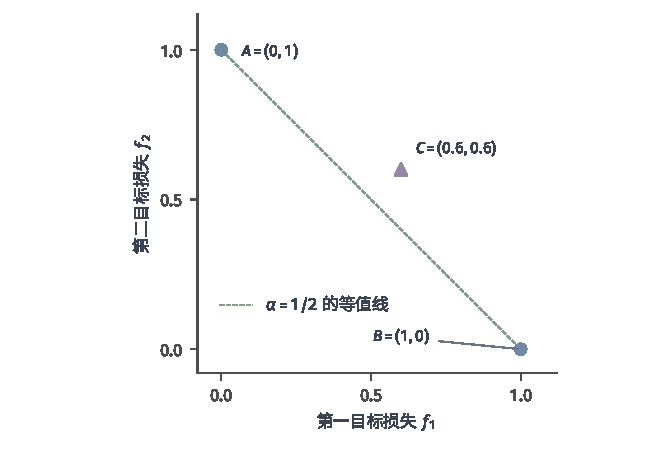
\includegraphics[width=112.0mm]{figures/00-shared/mathematical-preliminaries-upper/04-optimization/matplotlib/opt-pareto-weighted-sum/figure.pdf}
  \caption{三个精确可行损失向量。$A,B,C$互不支配，但对任意$\alpha\in[0,1]$，$C$的加权损失$0.6$都严格大于$\min\{\alpha,1-\alpha\}$；绿虚线为$\alpha=1/2$时通过$A,B$的等值线。Pareto最优不保证能由加权和选到。}
 \label{fig:opt-pareto-weighted-sum}
\end{figure}

\subsection{最小范数梯度组合法}

若当前希望同时改善所有指标，方向$\bm d$满足
\[
 \langle\nabla f_i(\bm w),\bm d\rangle<0\quad(\forall i)
\]
时称为\term{共同下降方向}的严格版本。把原点投影到梯度凸包上：
\[
 \bm\alpha^\star\in\arg\min_{\bm\alpha\in\bm\Delta_m}
 \frac12\left\|\sum_i\alpha_i\nabla f_i(\bm w)\right\|_2^2,
 \qquad
 \bar{\bm g}=\sum_i\alpha_i^\star\nabla f_i(\bm w).
\]
权重子问题是单纯形约束凸二次问题，凸包紧故投影向量$\bar{\bm g}$唯一（权重未必唯一）。

\begin{theorem}[无共同下降方向的一阶判定]
\label{thm:opt-common-descent}
对可微的$m$个目标，无约束点$\bm w$处不存在共同严格下降方向，当且仅当存在$\alpha_i\geq0$、$\sum_i\alpha_i=1$使$\sum_i\alpha_i\nabla f_i(\bm w)=\bm0$。
\end{theorem}

\begin{proof}
若零凸组合存在而$\bm d$使每个内积为负，加权内积也为负，矛盾。反之，若原点不在梯度凸包内，凸集外点分离给出与每个梯度内积同号的方向，必要时取反即为共同严格下降方向。
\end{proof}

若$\bar{\bm g}\neq\bm0$，投影最优性给$\langle\bar{\bm g},\nabla f_i-\bar{\bm g}\rangle\geq0$，取$\bm d=-\bar{\bm g}$则每个方向导数至多$-\|\bar{\bm g}\|^2$；各目标$L_i$光滑时$0<\eta<2/\max_iL_i$使这一步共同下降，未知常数时要求每个目标都通过回溯。例$f_1=((x-1)^2+y^2)/2$、$f_2=((x+1)^2+y^2)/2$在$(0,1)$的梯度为$(-1,1),(1,1)$，最小范数平均$(0,1)$、步长$1$到$(0,0)$，两项各降$1/2$；在$(0,0)$零已在两梯度之间，不能再共同下降。该判据只排除一阶共同改善（两目标均为$-x^2$在$0$处即为反例），有约束时还要限制方向可行。

\subsection{阈值约束法与有限候选实现}

若某些指标有硬上限，保留一个指标作目标、其余写成约束：
\[
 \min\{f_j(\bm w):\bm w\in C,\ f_i(\bm w)\leq B_i\ (i\neq j)\}.
\]
其全局最小点至少弱Pareto最优（全部指标严格更小的候选会连$f_j$一起改善），但未必Pareto，需要时在最优候选中再排除支配点。

\paragraph{有限候选的码率—失真选择。}
给有限方案的码率$R_k$、失真$D_k$（均越小越好），预算题枚举$\min\{D_k:R_k\leq B\}$，价格题枚举$\min_k(D_k+\lambda R_k)$。把三点$(R,D)=(0,1),(1,0),(0.6,0.6)$用于$B=0.6$：第三点以$D=0.6$入选，而任何$\lambda$都不选它——预算题与价格题覆盖不同答案。点间线段只有在混合实际允许（编码块或时间可拼接）并计入拼接成本时才有可行含义；若总代价可加且各块独立，固定$\lambda$时$\min\sum_i(D_i+\lambda R_i)=\sum_i\min(D_i+\lambda R_i)$，但总预算约束仍耦合各块。只有在另外建立了可由支撑线达到的光滑下降曲线$D(R)$后，内部最优才满足$D'(R)+\lambda=0$；不对有限点的角点直接求导。概率率失真函数还需信息论前提。

\subsection{原多目标问题的最优性与解集}

定理~\ref{thm:opt-common-descent}是算法无关的一阶证书；它不保证全局Pareto最优。若每个目标凸，零梯度凸组合使相应加权和全局最小，给弱Pareto结论；严格正权重再加强为Pareto。$f_1(x)=0,f_2(x)=x^2$在$x=1$满足一阶判据却被$x=0$支配，说明零权的边界。非空紧可行集与连续指标下，严格正权标量目标的全局最小点存在且Pareto最优，保证至少有一个Pareto点；紧性负责达到，正权负责排除支配。

\subsection{进展、敏感性与预算}

加权和沿指定偏好求解、不保证每项逐轮下降；最小范数法在合格条件下保证当前共同下降，零向量只给一阶证书；有限枚举在给定候选与预算内返回最小失真。改变权重时标量解可连续移动，改变预算时答案可在$R_k$跨过阈值处离散切换。枚举、标量求解与梯度子问题各有成本，回溯还要对每个指标重复评价。

\section{极小极大优化}

在鲁棒训练的一个样本$(\bm x,y)$上，固定参数$\bm w$后考虑允许集合$\Delta$中的特征扰动$\bm\delta$；标签$y$不变。若$\Delta$非空紧、损失关于$\bm\delta$连续，内层最大值达到，外层再降低这种最坏损失。一般形式为
\begin{equation}
 \min_{\bm w\in W}\max_{\bm z\in Z}\phi(\bm w,\bm z).
 \label{eq:opt-minimax}
\end{equation}
外层先选$\bm w$，内层看到它后选使损失最大的$\bm z$；外层最小化的是最坏响应值，交换次序一般改变值。

\subsection{鞍点、间隙与最值交换}

\begin{definition}[极小极大鞍点]
\label{def:opt-minimax-saddle}
点$(\bm w^\star,\bm z^\star)$若对所有$\bm w\in W,\bm z\in Z$满足
\[
 \phi(\bm w^\star,\bm z)\leq\phi(\bm w^\star,\bm z^\star)
 \leq\phi(\bm w,\bm z^\star),
\]
称为\term{极小极大鞍点}（minimax saddle point）。
\end{definition}

这是两组变量承担相反优化方向时的全局最优响应关系，不是多元微积分中由Hessian正负曲率定义的微分鞍点。定义
\[
 P(\bm w)=\sup_{\bm z\in Z}\phi(\bm w,\bm z),\qquad
 D(\bm z)=\inf_{\bm w\in W}\phi(\bm w,\bm z),
\]
总有$D(\bm z)\leq P(\bm w)$，非负的\term{原始--对偶间隙}$P(\bm w)-D(\bm z)$为零时该候选对满足鞍点不等式。

\begin{theorem}[紧凸凹条件下的最值交换]
若$W,Z$非空、紧且凸，$\phi$连续，对固定$\bm z$关于$\bm w$凸、对固定$\bm w$关于$\bm z$凹，则
\[
 \min_{\bm w\in W}\max_{\bm z\in Z}\phi
 =\max_{\bm z\in Z}\min_{\bm w\in W}\phi,
\]
且两侧最值均达到。
\end{theorem}

证明思路（完整分离论证较长）：任取$c$小于左侧值，紧性给出有限个$\bm z_1,\ldots,\bm z_k$使每个$\bm w$至少在一项超过$c$；考虑由这些值定义的向上封闭凸集，严格分离给出非负归一权重，再用关于$\bm z$的凹性把加权响应合成为$Z$中一个$\bar{\bm z}$，推出右侧值大于$c$；令$c$趋于左侧值并结合弱对偶即得等号，连续性保证两侧达到。紧性、连续性与凸凹性各司其职，一般非凸对抗训练不能直接套用。

\subsection{同时梯度下降—上升法}

在可微延拓下，两方在同一旧点各取一次偏梯度：
\[
 \bm w^+=\Pi_W(\bm w-\eta\nabla_{\bm w}\phi(\bm w,\bm z)),\qquad
 \bm z^+=\Pi_Z(\bm z+\eta\nabla_{\bm z}\phi(\bm w,\bm z)).
\]
两方向都从同一旧点计算。取$W=Z=[-1,1]$、$\phi(x,z)=xz$：$P(x)=|x|$、$D(z)=-|z|$，唯一鞍点$(0,0)$，候选间隙为$|x|+|z|$。不投影时
\[
 (x^+)^2+(z^+)^2=(1+\eta^2)(x^2+z^2),
\]
每个非零初值向外旋转（离开盒后已不是可行候选）。加盒投影也不收敛：$\eta=1$从$(1,0)$出发沿八个角点和边中点周期循环，间隙始终不小于$1$。值的存在定理不替代具体算法的收敛定理。

\subsection{外梯度法}

外梯度先试探、再用试探点方向从旧点校正：
\[
 \bar{\bm u}=\Pi_K(\bm u-\eta\bm F(\bm u)),\qquad
 \bm u^+=\Pi_K(\bm u-\eta\bm F(\bar{\bm u})),
\]
其中$\bm u=(\bm w,\bm z)$、$\bm F(\bm u)=(\nabla_{\bm w}\phi,-\nabla_{\bm z}\phi)$、$K=W\times Z$，每轮两次方向求值与两次投影。在双线性例中投影未激活时更新矩阵为$\begin{smallmatrix}1-\eta^2&-\eta\\ \eta&1-\eta^2\end{smallmatrix}$，距离平方每步乘
\[
 1-\eta^2+\eta^4<1\qquad(0<\eta<1).
\]
取$\eta=1/2$、$\|\bm u^{(0)}\|_2\leq1/2$：试探点范数至多$\sqrt5/4<1$、校正点范数递减，归纳得两次投影都不激活且距离几何收缩，故趋于鞍点、间隙趋零。这是该例的可核验改善；一般问题还需梯度映射的单调性、Lipschitz等条件，多算一次方向本身不是普遍收敛定理。

图~\ref{fig:vol1-add-minimax-rotation}比较两种更新的轨迹与距离。
\begin{figure}[!htb]
  \centering
  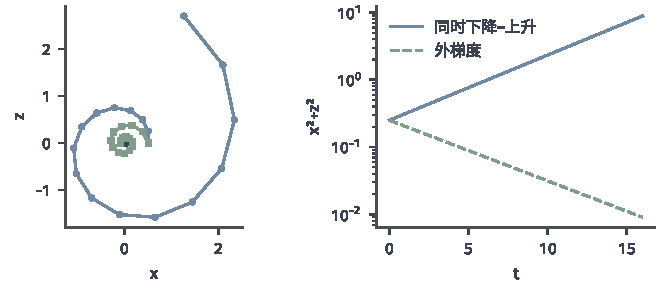
\includegraphics[width=112mm]{figures/00-shared/mathematical-preliminaries-upper/00-shared/matplotlib/mathematical-language-combinatorics-analysis-optimization-comprehension-additions/minimax-rotation.pdf}
  \caption{对$\phi(x,z)=xz$取$\eta=1/2$、初值$(1/2,0)$。蓝线为无投影同时下降--上升，距离平方每步乘$1+\eta^2$；绿线为外梯度，每步乘$1-\eta^2+\eta^4<1$。蓝线离盒后不是可行候选，绿线试探与校正始终在盒内。}
  \label{fig:vol1-add-minimax-rotation}
\end{figure}

\subsection{结果、过程与预算}

紧凸凹条件保证值交换与鞍点达到，却不指定轨迹；同一双线性盒任务上同时法循环、外梯度在特定初值与步长内收缩，故存在性与算法收敛分别报告。比较预算时同时法每轮两组偏梯度，外梯度每轮两次求值加两次投影；若全局间隙还需内层最优响应，其求解成本也要计入。

\section{双层优化}
\label{sec:opt-bilevel}

\term{双层优化}中，有些决策必须先经过一次学习才能评价：外层变量$\bm\theta\in\Theta\subseteq\mathbb R^p$（如正则强度）先改变内层训练问题，训练后参数再给外层损失。令内层变量$\bm w\in\mathbb R^d$。若内层有多个最小点，只写$\bm w^\star(\bm\theta)\in\arg\min_{\bm w}L_{\rm in}$没有定义单值映射，可规定乐观（取外层值下确界）或悲观（上确界）选解，或给定由初始化与算法决定的选择规则$S$。下文假设内层最小解唯一或已给定单值选择：
\[
 \bm w^\star(\bm\theta)=S(\bm\theta)\in\arg\min_{\bm w}L_{\rm in}(\bm w,\bm\theta),
\]
外层实际比较的是内层选解经过评价后的复合目标
\begin{equation}
 J(\bm\theta)=L_{\rm out}(\bm w^\star(\bm\theta),\bm\theta).
 \label{eq:opt-bilevel-objective}
\end{equation}
例$L_{\rm in}(w,\theta)=(w^2-1)^2$的内层最小点恒为$\{-1,1\}$，外层$(w-\theta)^2/2$在$\theta=1$时乐观值$0$、悲观值$2$：内层最优值相同不消除外层歧义。内层最大化可改写为最小化负目标；鲁棒训练的内外层角色（内层选扰动、外层调参数）与超参调优不同，不能套用同一说明。

\subsection{迭代展开法}

\subsubsection{梯度下降的展开与外层方向}

对内层更新$\bm w^{(t+1)}=\bm w^{(t)}-\eta\nabla_{\bm w}L_{\rm in}(\bm w^{(t)},\bm\theta)$（二阶连续可微、固定步长），定义
\[
 \bm A^{(t)}=\bm I-\eta\nabla_{\bm w,\bm w}^2L_{\rm in},\qquad
 \bm B^{(t)}=\nabla_{\bm w,\bm\theta}^2L_{\rm in},
 \qquad
 \bm D_t=\frac{\mathrm d\bm w^{(t)}}{\mathrm d\bm\theta},
\]
则$\bm D_{t+1}=\bm A^{(t)}\bm D_t-\eta\bm B^{(t)}$。有限步目标$J_T(\bm\theta)=L_{\rm out}(\bm w^{(T)}(\bm\theta),\bm\theta)$的外层梯度为
\[
 \nabla_{\bm\theta}J_T
 =\bm D_T^\top\nabla_{\bm w}L_{\rm out}
 +\nabla_{\bm\theta}L_{\rm out}.
\]
存储大时等价地反向累计：保存$\bm q_T=\nabla_{\bm w}L_{\rm out}$，逆向做$\bm h\leftarrow\bm h-\eta(\bm B^{(t)})^\top\bm q_{t+1}$、$\bm q_t=(\bm A^{(t)})^\top\bm q_{t+1}$，再加初值依赖项。

\subsubsection{带历史状态、截断与数值核验}

带动量等优化器时展开对象须是完整状态$\bm z^{(t)}=(\bm w^{(t)},\bm s^{(t)})$：$\bm D_z^{t+1}=(\partial_{\bm z}\mathcal U_t)\bm D_z^t+\partial_\theta\mathcal U_t$；符号、裁剪分支与平方根切换处要检查复合映射的可微范围。前向仍跑$T$步、只截断反向$\ell$步，舍去的是Jacobian乘积，方向误差不超过$\|\nabla_{\bm w}L_{\rm out}\|\,\|\bm A^{T-1}\cdots\bm A^{T-\ell}\|\,\|\bm D_{T-\ell}\|$；而减少前向步数改变的是$J_T$本身。用$L_{\rm in}=(w-\theta)^2/2$、$w^{(0)}=0$、$\eta=1/2$：两步得$w^{(2)}=3\theta/4$，外层$(w-1)^2/2$在$\theta=2$的梯度为$3/8$；理想内层解$w^\star=\theta$对应梯度为$1$。两者都正确，差别在求导对象——点收敛不自动推出导数收敛。

图~\ref{fig:opt-bilevel-target-chains}把这两个目标的计算链放在同一画面中。有限步链把两次实际更新纳入复合函数，理想链则直接使用精确内层解；二者即使共享内层损失与外层评价，导数也对应不同的目标。

\begin{figure*}[htbp]
 \centering
 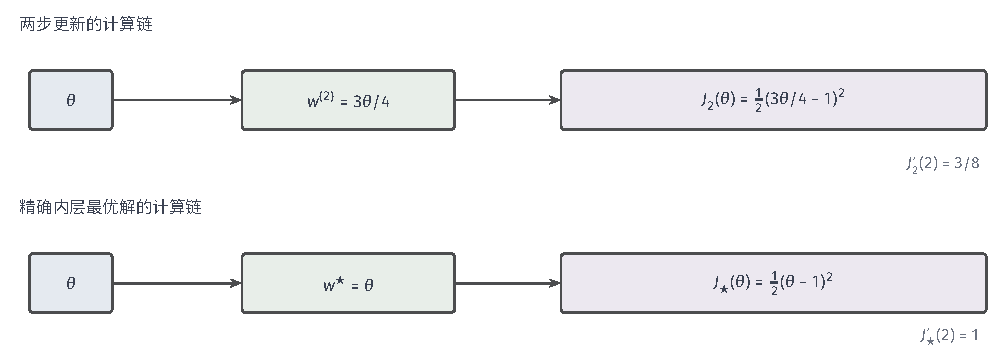
\includegraphics[width=168.998mm]{figures/00-shared/mathematical-preliminaries-upper/04-optimization/tikz/opt-bilevel-target-chains/figure.pdf}
 \caption{同一二次内层目标的两条计算链。固定$w^{(0)}=0$、步长$1/2$，两次更新产生$w^{(2)}=3\theta/4$；精确最优解则为$w^\star=\theta$。外层都读取$(w-1)^2/2$，但两个复合目标不同，故在$\theta=2$处分别得到导数$3/8$与$1$。有限步算法的求导与精确解分支的求导各自对应自己的目标。}
 \label{fig:opt-bilevel-target-chains}
\end{figure*}

\subsection{隐式微分法}

\subsubsection{选定分支的可微性与目标归属}

固定局部最小点$\widehat{\bm w}_0$（无约束内点），其满足$\nabla_{\bm w}L_{\rm in}=\bm0$。若$\bm H_{ww}=\nabla_{\bm w,\bm w}^2L_{\rm in}$可逆，隐函数定理给出局部可微驻点分支；非退化局部最小点处$\bm H_{ww}\succ\bm0$，分支保持严格局部最小。但隐函数定理不承担全局归属：只有该分支始终是规定的全局选解，才有$\widehat J=J$；Hessian奇异是局部导数问题，分支非凸不全局最优是目标归属问题，提高求解精度都不能修复。

\subsubsection{隐式导数、伴随计算与两类残差}

对驻点方程关于$\bm\theta$求导：
\[
 \bm H_{ww}\widehat{\bm D}+\bm H_{w\theta}=\bm0
 \quad\Longrightarrow\quad
 \widehat{\bm D}=-\bm H_{ww}^{-1}\bm H_{w\theta},
\]
代入外层链式法则得\term{隐式超梯度}
\begin{equation}
 \nabla_{\bm\theta}\widehat J
 =\nabla_{\bm\theta}L_{\rm out}
 -\bm H_{w\theta}^\top\bm H_{ww}^{-\top}\nabla_{\bm w}L_{\rm out},
 \label{eq:opt-implicit-hypergradient}
\end{equation}
实践中解伴随方程$\bm H_{ww}^\top\bm v=\nabla_{\bm w}L_{\rm out}$而不显式求逆。

近似内层点的残差$\bm r_{\rm in}=\nabla_{\bm w}L_{\rm in}(\widetilde{\bm w},\bm\theta)$在邻域$\bm H_{ww}\succeq\mu\bm I$下给点误差$\|\widetilde{\bm w}-\widehat{\bm w}\|\leq\|\bm r_{\rm in}\|/\mu$；同点线性系统残差$\bm r_{\rm lin}=\widetilde{\bm H}^\top\widetilde{\bm v}-\widetilde{\bm g}$给伴随误差。设超梯度作为$\bm w$的函数在该邻域Lipschitz常数为$C$，总误差满足
\begin{equation}
 \|\widetilde{\nabla_{\bm\theta}\widehat J}
 -\nabla_{\bm\theta}\widehat J\|_2
 \leq\frac{C}{\mu}\|\bm r_{\rm in}\|_2
 +\frac{\|\widetilde{\bm B}\|_2}{\mu}\|\bm r_{\rm lin}\|_2.
 \label{eq:opt-hypergradient-two-residuals}
\end{equation}
两项分别来自内层点不准与同点伴随未解准；小$\mu$同时放大二者。取得外层方向后仍要按$\widehat J$的光滑性和可行集执行自己的步长与停止。

\subsection{原双层问题的选解、结果与预算}

原双层问题的外层最小点存在要逐参数核验：内层适当下半连续且有紧下水平集时内层解达到，适当闭强凸给内层唯一，但这些不自动给外层最小点，还需选解规则连续、外层损失连续与参数域紧等条件。结果评价先固定针对$J_T$、$\widehat J$还是$J$：展开法给有限步目标的导数，隐式法给合格分支的导数，$3/8$与$1$不是数值误差而是不同目标的正确导数。总预算比较须合计前向内层迭代、存储或重算、反向传播、伴随求解与外层迭代；压低一种残差未必控制完整超梯度误差。

\section{本章小结}

多目标先用支配排除共同劣势，再用权重、共同方向或阈值规定取舍；梯度凸包含零只是一阶证书，未支撑Pareto点与有限工作点不能被加权和自动覆盖。极小极大先规定响应次序，用全局鞍点不等式与候选间隙检验输出；紧凸凹使最值可交换，但同时下降--上升仍可能旋转，外梯度的收缩依赖额外条件。双层先规定内层选解，再区分有限步目标$J_T$、局部分支$\widehat J$与理想全局选解$J$；展开梯度与隐式超梯度各自忠实于其目标，内层驻点残差与伴随残差要同时控制。最优化部分至此覆盖了问题定义、存在与最优性、光滑与非光滑求解、约束证书、预算近似与决策结构；后续函数空间章将把有限维参数推广到函数，随机逼近与策略评价则会复用本章的对偶与鞍点语言。

